% Options for packages loaded elsewhere
\PassOptionsToPackage{unicode}{hyperref}
\PassOptionsToPackage{hyphens}{url}
%
\documentclass[
]{book}
\usepackage{amsmath,amssymb}
\usepackage{lmodern}
\usepackage{ifxetex,ifluatex}
\ifnum 0\ifxetex 1\fi\ifluatex 1\fi=0 % if pdftex
  \usepackage[T1]{fontenc}
  \usepackage[utf8]{inputenc}
  \usepackage{textcomp} % provide euro and other symbols
\else % if luatex or xetex
  \usepackage{unicode-math}
  \defaultfontfeatures{Scale=MatchLowercase}
  \defaultfontfeatures[\rmfamily]{Ligatures=TeX,Scale=1}
\fi
% Use upquote if available, for straight quotes in verbatim environments
\IfFileExists{upquote.sty}{\usepackage{upquote}}{}
\IfFileExists{microtype.sty}{% use microtype if available
  \usepackage[]{microtype}
  \UseMicrotypeSet[protrusion]{basicmath} % disable protrusion for tt fonts
}{}
\makeatletter
\@ifundefined{KOMAClassName}{% if non-KOMA class
  \IfFileExists{parskip.sty}{%
    \usepackage{parskip}
  }{% else
    \setlength{\parindent}{0pt}
    \setlength{\parskip}{6pt plus 2pt minus 1pt}}
}{% if KOMA class
  \KOMAoptions{parskip=half}}
\makeatother
\usepackage{xcolor}
\IfFileExists{xurl.sty}{\usepackage{xurl}}{} % add URL line breaks if available
\IfFileExists{bookmark.sty}{\usepackage{bookmark}}{\usepackage{hyperref}}
\hypersetup{
  pdftitle={Simulation and Modelling to Understand Change},
  pdfauthor={Manuele Leonelli},
  hidelinks,
  pdfcreator={LaTeX via pandoc}}
\urlstyle{same} % disable monospaced font for URLs
\usepackage{color}
\usepackage{fancyvrb}
\newcommand{\VerbBar}{|}
\newcommand{\VERB}{\Verb[commandchars=\\\{\}]}
\DefineVerbatimEnvironment{Highlighting}{Verbatim}{commandchars=\\\{\}}
% Add ',fontsize=\small' for more characters per line
\usepackage{framed}
\definecolor{shadecolor}{RGB}{248,248,248}
\newenvironment{Shaded}{\begin{snugshade}}{\end{snugshade}}
\newcommand{\AlertTok}[1]{\textcolor[rgb]{0.94,0.16,0.16}{#1}}
\newcommand{\AnnotationTok}[1]{\textcolor[rgb]{0.56,0.35,0.01}{\textbf{\textit{#1}}}}
\newcommand{\AttributeTok}[1]{\textcolor[rgb]{0.77,0.63,0.00}{#1}}
\newcommand{\BaseNTok}[1]{\textcolor[rgb]{0.00,0.00,0.81}{#1}}
\newcommand{\BuiltInTok}[1]{#1}
\newcommand{\CharTok}[1]{\textcolor[rgb]{0.31,0.60,0.02}{#1}}
\newcommand{\CommentTok}[1]{\textcolor[rgb]{0.56,0.35,0.01}{\textit{#1}}}
\newcommand{\CommentVarTok}[1]{\textcolor[rgb]{0.56,0.35,0.01}{\textbf{\textit{#1}}}}
\newcommand{\ConstantTok}[1]{\textcolor[rgb]{0.00,0.00,0.00}{#1}}
\newcommand{\ControlFlowTok}[1]{\textcolor[rgb]{0.13,0.29,0.53}{\textbf{#1}}}
\newcommand{\DataTypeTok}[1]{\textcolor[rgb]{0.13,0.29,0.53}{#1}}
\newcommand{\DecValTok}[1]{\textcolor[rgb]{0.00,0.00,0.81}{#1}}
\newcommand{\DocumentationTok}[1]{\textcolor[rgb]{0.56,0.35,0.01}{\textbf{\textit{#1}}}}
\newcommand{\ErrorTok}[1]{\textcolor[rgb]{0.64,0.00,0.00}{\textbf{#1}}}
\newcommand{\ExtensionTok}[1]{#1}
\newcommand{\FloatTok}[1]{\textcolor[rgb]{0.00,0.00,0.81}{#1}}
\newcommand{\FunctionTok}[1]{\textcolor[rgb]{0.00,0.00,0.00}{#1}}
\newcommand{\ImportTok}[1]{#1}
\newcommand{\InformationTok}[1]{\textcolor[rgb]{0.56,0.35,0.01}{\textbf{\textit{#1}}}}
\newcommand{\KeywordTok}[1]{\textcolor[rgb]{0.13,0.29,0.53}{\textbf{#1}}}
\newcommand{\NormalTok}[1]{#1}
\newcommand{\OperatorTok}[1]{\textcolor[rgb]{0.81,0.36,0.00}{\textbf{#1}}}
\newcommand{\OtherTok}[1]{\textcolor[rgb]{0.56,0.35,0.01}{#1}}
\newcommand{\PreprocessorTok}[1]{\textcolor[rgb]{0.56,0.35,0.01}{\textit{#1}}}
\newcommand{\RegionMarkerTok}[1]{#1}
\newcommand{\SpecialCharTok}[1]{\textcolor[rgb]{0.00,0.00,0.00}{#1}}
\newcommand{\SpecialStringTok}[1]{\textcolor[rgb]{0.31,0.60,0.02}{#1}}
\newcommand{\StringTok}[1]{\textcolor[rgb]{0.31,0.60,0.02}{#1}}
\newcommand{\VariableTok}[1]{\textcolor[rgb]{0.00,0.00,0.00}{#1}}
\newcommand{\VerbatimStringTok}[1]{\textcolor[rgb]{0.31,0.60,0.02}{#1}}
\newcommand{\WarningTok}[1]{\textcolor[rgb]{0.56,0.35,0.01}{\textbf{\textit{#1}}}}
\usepackage{longtable,booktabs,array}
\usepackage{calc} % for calculating minipage widths
% Correct order of tables after \paragraph or \subparagraph
\usepackage{etoolbox}
\makeatletter
\patchcmd\longtable{\par}{\if@noskipsec\mbox{}\fi\par}{}{}
\makeatother
% Allow footnotes in longtable head/foot
\IfFileExists{footnotehyper.sty}{\usepackage{footnotehyper}}{\usepackage{footnote}}
\makesavenoteenv{longtable}
\usepackage{graphicx}
\makeatletter
\def\maxwidth{\ifdim\Gin@nat@width>\linewidth\linewidth\else\Gin@nat@width\fi}
\def\maxheight{\ifdim\Gin@nat@height>\textheight\textheight\else\Gin@nat@height\fi}
\makeatother
% Scale images if necessary, so that they will not overflow the page
% margins by default, and it is still possible to overwrite the defaults
% using explicit options in \includegraphics[width, height, ...]{}
\setkeys{Gin}{width=\maxwidth,height=\maxheight,keepaspectratio}
% Set default figure placement to htbp
\makeatletter
\def\fps@figure{htbp}
\makeatother
\setlength{\emergencystretch}{3em} % prevent overfull lines
\providecommand{\tightlist}{%
  \setlength{\itemsep}{0pt}\setlength{\parskip}{0pt}}
\setcounter{secnumdepth}{5}
\usepackage{booktabs}
\ifluatex
  \usepackage{selnolig}  % disable illegal ligatures
\fi
\usepackage[]{natbib}
\bibliographystyle{apalike}

\title{Simulation and Modelling to Understand Change}
\author{Manuele Leonelli}
\date{2021-02-01}

\begin{document}
\maketitle

{
\setcounter{tocdepth}{1}
\tableofcontents
}
\hypertarget{preface}{%
\chapter*{Preface}\label{preface}}
\addcontentsline{toc}{chapter}{Preface}

These are lecture notes for the module \emph{Simulation and Modelling to Understand Change} given in the School of Human Sciences and Technology at IE University, Madrid, Spain. The module is given in the 2nd semester of the 1st year of the bachelor in Data \& Business Analytics. Knowledge of basic elements of R programming as well as probability and statistics is assumed.

\hypertarget{intro}{%
\chapter{Introduction}\label{intro}}

The first introductory chapter gives an overview of simulation, what it is, what it can be used for, as well as some examples.

\hypertarget{what-is-simulation}{%
\section{What is simulation}\label{what-is-simulation}}

A \emph{simulation} is an imitation of the dynamics of a real-world process or system over time. Although simulation could potentially still be done ``by hand'', nowadays it almost always implicitly requires the use of a computer to create an artificial history of a system to draw inferences about its characteristics and workings.

The behavior of the system is studied by constructing a \emph{simulation model}, which usually takes the form of a set of assumptions about the workings of the system. Once developed, a simulation model can be used for a variety of tasks, including:

\begin{itemize}
\item
  Investigate the behaviour of the system under a wide array of scenarios. This is also often referred to as ``what-if'' analyses;
\item
  Changes to the system can be simulated before implementation to predict their impact in real-world;
\item
  During the design stage of a system, meaning while it is being built, simulation can be used to guide its construction.
\end{itemize}

Computer simulation has been used in a variety of domains, including manifacturing, health care, transport system, defense and management science, among many others.

\hypertarget{a-simple-simulation-model}{%
\subsection{A simple simulation model}\label{a-simple-simulation-model}}

Suppose we decided to open a donut shop and are unsure about how many employees to hire to sell donuts to costumers. The operations of our little shop is the real-world system whose behavior we want to understand. Given that the shop is not operating yet, only a simulation model can provide us with insights.

We could of course devise models of different complexities, but for now suppose that we are happy with a simple model where we have the following elements:

\begin{itemize}
\item
  costumers that arrive at our shop at a particular rate;
\item
  employees (of a number to be given as input) that take a specific time to serve costumers.
\end{itemize}

Implicitly, we are completely disregarding the number of donuts available in our shop and assuming that we have an infinite availability of these. Of course, in a more complex simulation model we may want to also include this element to give a more realistic description of the system.

\hypertarget{why-simulate}{%
\subsection{Why simulate?}\label{why-simulate}}

An alternative approach to computer simulation is direct experimentation. In the bagel shop setting, we could wait for the shop to open and observe its workings by having a different number of employees on different days. Considered against real experimentation, simulation has the following advantages:

\begin{itemize}
\item
  It is \emph{cheaper} to implement and does not require a disruption of the real-world system;
\item
  It is \emph{faster} to implement and time can be compressed or expanded to allow for a speed-up or a slow-down of the system of interest;
\item
  It can be \emph{replicated} multiple times and the workings of the systems can be observed a large number of times;
\item
  It is \emph{safe} since it does not require an actual disruption of the system;
\item
  It is \emph{ethical} and \emph{legal} since it can implement changes in policies that would be unethical or illegal to do in real-world.
\end{itemize}

Another alternative is to use a mathematical model representing the system. However, it is often infeasible, if not impossible, to come up with an exact mathematical model which can faithfully represent the system under study.

\hypertarget{types-of-simulations}{%
\section{Types of simulations}\label{types-of-simulations}}

Before starting the construction of a simulation model, we need to decide upon the principal characteristics of that model. There are various choices to be made, which depend upon the system we are trying to understand.

\hypertarget{stochastic-vs-deterministic-simulations}{%
\subsection{Stochastic vs deterministic simulations}\label{stochastic-vs-deterministic-simulations}}

A model is \emph{deterministic} if its behavior is entirely predictable. Given a set of inputs, the model will result in a unique set of outputs. A model is \emph{stochastic} if it has random variables as inputs, and consequently also its outputs are random.

Consider the donut shop example. In a deterministic model we would for instance assume that a new customer arrives every 5 minutes and an employee takes 2 minutes to serve a customer. In a stochastic model we would on the other hand assume that the arrival times and the serving time follows some random variables: for instance, normal distributions with some mean and variance parameters.

In this course we will only consider stochastic simulation, but for illustration we consider now an example of a deterministic simulation.

A social media influencer decides to open a new page and her target is to reach 10k followers in 10 weeks. Given her past experience, she assumes that each week she will get 1.5k new followers that had never followed the page and of her current followers she believes 10\% will stop following the page each week. However, 20\% of those that the left the page in the past will join again each week. Will she reach her target?

To answer this question we can construct a deterministic simulation. Let \(F_t\) the number of followers at week \(t\) and \(U_t\) the number of users that are unfollowing the profile at week \(t\). Then
\[
F_t = F_{t-1} + 1500 - L_{t} + R_{t}, \hspace{1cm} U_t= U_{t-1} + L_{t} - R_{t}
\]
where \(L_{t}=0.1\cdot F_{t-1}\) is the number of unfollowers from time \(t-1\) to time \(t\), and \(R_{t}=0.2\cdot U_{t-1}\) is the number of users that follow the page back from time \(t-1\) to time \(t\).

To compute the number of followers after ten weeks we can use the R code below. It does not matter if you do not understand it now, we will review R coding in the next chapters.

\begin{Shaded}
\begin{Highlighting}[]
\NormalTok{Ft }\OtherTok{\textless{}{-}}\NormalTok{ Ut }\OtherTok{\textless{}{-}}\NormalTok{ Lt }\OtherTok{\textless{}{-}}\NormalTok{ Rt }\OtherTok{\textless{}{-}} \FunctionTok{rep}\NormalTok{(}\DecValTok{0}\NormalTok{,}\DecValTok{11}\NormalTok{)}
\ControlFlowTok{for}\NormalTok{ (i }\ControlFlowTok{in} \DecValTok{2}\SpecialCharTok{:}\DecValTok{11}\NormalTok{)\{}
\NormalTok{  Lt[i] }\OtherTok{\textless{}{-}} \FloatTok{0.1}\SpecialCharTok{*}\NormalTok{Ft[i}\DecValTok{{-}1}\NormalTok{]}
\NormalTok{  Rt[i] }\OtherTok{\textless{}{-}} \FloatTok{0.2}\SpecialCharTok{*}\NormalTok{Ut[i}\DecValTok{{-}1}\NormalTok{]}
\NormalTok{  Ut[i] }\OtherTok{\textless{}{-}}\NormalTok{ Ut[i}\DecValTok{{-}1}\NormalTok{] }\SpecialCharTok{+}\NormalTok{ Lt[i] }\SpecialCharTok{{-}}\NormalTok{ Rt[i]}
\NormalTok{  Ft[i] }\OtherTok{\textless{}{-}}\NormalTok{ Ft[i}\DecValTok{{-}1}\NormalTok{] }\SpecialCharTok{+} \DecValTok{1500} \SpecialCharTok{{-}}\NormalTok{ Lt[i] }\SpecialCharTok{+}\NormalTok{ Rt[i]}
\NormalTok{\}}
\NormalTok{result }\OtherTok{\textless{}{-}} \FunctionTok{data.frame}\NormalTok{(}\StringTok{"Followers"} \OtherTok{=}\NormalTok{ Ft, }\StringTok{"Total Unfollowers"} \OtherTok{=}\NormalTok{ Ut,}
           \StringTok{"Weekly Unfollowers"} \OtherTok{=}\NormalTok{ Ut, }\StringTok{"Weekly Returns"} \OtherTok{=}\NormalTok{ Rt)}
\end{Highlighting}
\end{Shaded}

The dataframe \texttt{result} is reported in Table \ref{tab:insta}, showing that she will be able to hit her target of 10k followers since she will have 11619 followers. If we run again the simulation we will obtain the exact same results: there is no stochasticity/uncertainty about the outcome.

\begin{table}

\caption{\label{tab:insta}Dataframe `result` from the social media deterministic simulation}
\centering
\begin{tabular}[t]{rrrr}
\toprule
Followers & Total.Unfollowers & Weekly.Unfollowers & Weekly.Returns\\
\midrule
0.000 & 0.000 & 0.000 & 0.0000\\
1500.000 & 0.000 & 0.000 & 0.0000\\
2850.000 & 150.000 & 150.000 & 0.0000\\
4095.000 & 405.000 & 405.000 & 30.0000\\
5266.500 & 733.500 & 733.500 & 81.0000\\
\addlinespace
6386.550 & 1113.450 & 1113.450 & 146.7000\\
7470.585 & 1529.415 & 1529.415 & 222.6900\\
8529.409 & 1970.591 & 1970.591 & 305.8830\\
9570.587 & 2429.413 & 2429.413 & 394.1181\\
10599.411 & 2900.589 & 2900.589 & 485.8827\\
\addlinespace
11619.587 & 3380.413 & 3380.413 & 580.1179\\
\bottomrule
\end{tabular}
\end{table}

The above application could be transformed into a stochastic simulation by allowing the rate at which she gets new followers, unfollowers etc. to be random variables of which we do not know the exact value.

\hypertarget{static-vs-dynamic-simulations}{%
\subsection{Static vs dynamic simulations}\label{static-vs-dynamic-simulations}}

Simulation models that represent the system at a particular point in time only are called \emph{static}. This type of simulations are often called as \emph{Monte Carlo simulations} and will be the focus of later chapters.

\emph{Dynamic} simulation models represent systems as they evolve over time. The simulation of the donut shop during its working hours is an example of a dynamic model.

\hypertarget{discrete-vs-continuous-simulations}{%
\subsection{Discrete vs continuous simulations}\label{discrete-vs-continuous-simulations}}

Dynamic simulations can be further categorized into discrete or continuous.

\emph{Discrete} simulation models are such that the variables of interest change only at a discrete set of points in time. The number of people queuing in the donut shop is an example of a discrete simulation. The number of customers changes only when a new customer arrives or when a customer has been served. Figure 1.1 gives an illustration of the discrete nature of the number of customers queuing in the donut shop.

\begin{figure}

{\centering 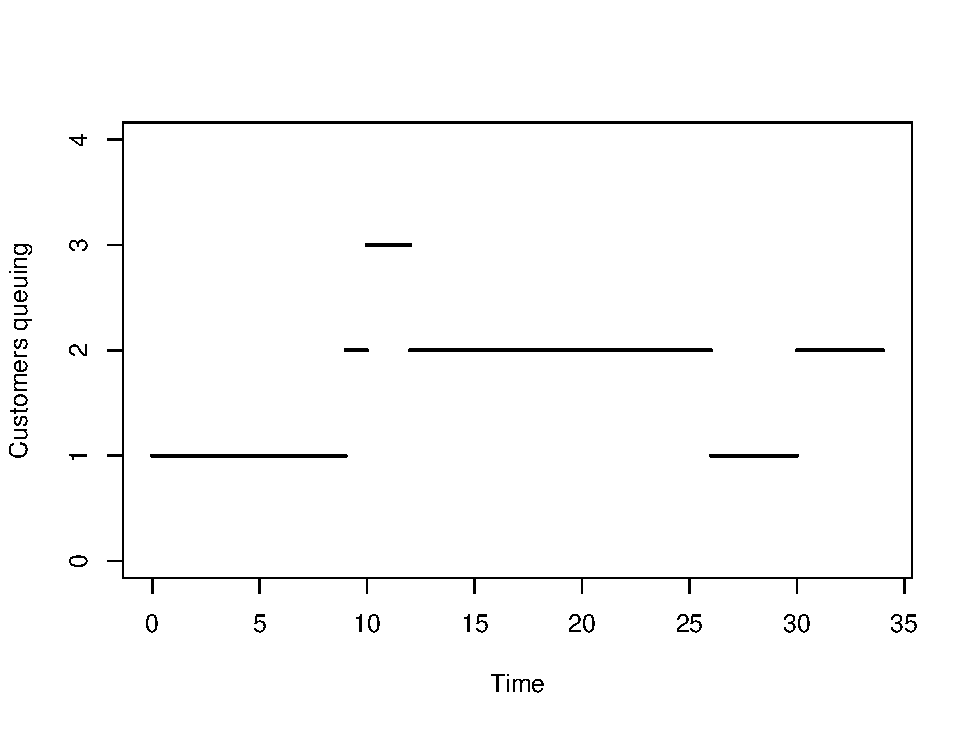
\includegraphics[width=0.8\linewidth]{SimBook_files/figure-latex/discrete-1} 

}

\caption{Example of a discrete dynamic simulation}\label{fig:discrete}
\end{figure}

Figure 1.1 further illustrates that for specific period of times the system does not change state, that is the number of customers queuing remains constant. It is therefore useless to inspect the system during those times where nothing changes. This prompts the way in which time is usually handled in dynamic discrete simulations, using the so-called \emph{next-event technique}. The model is only examined and updated when the system is due to change. These changes are usually called \emph{events}. Looking at Figure 1.1 at time zero there is an event: a customer arrives; at time nine another customer arrives; at time ten another customer arrives; at time twelve a customer is served; and so on. All these are examples of events.

\emph{Continuous} simulation models are such that the variables of interest change continuously over time. Suppose for instance a simulation model for a car journey was created where the interest is on the speed of the car throughout the journey. Then this would be a continuous simulation model. Figure 1.2 gives an illustration of this.

\begin{figure}

{\centering 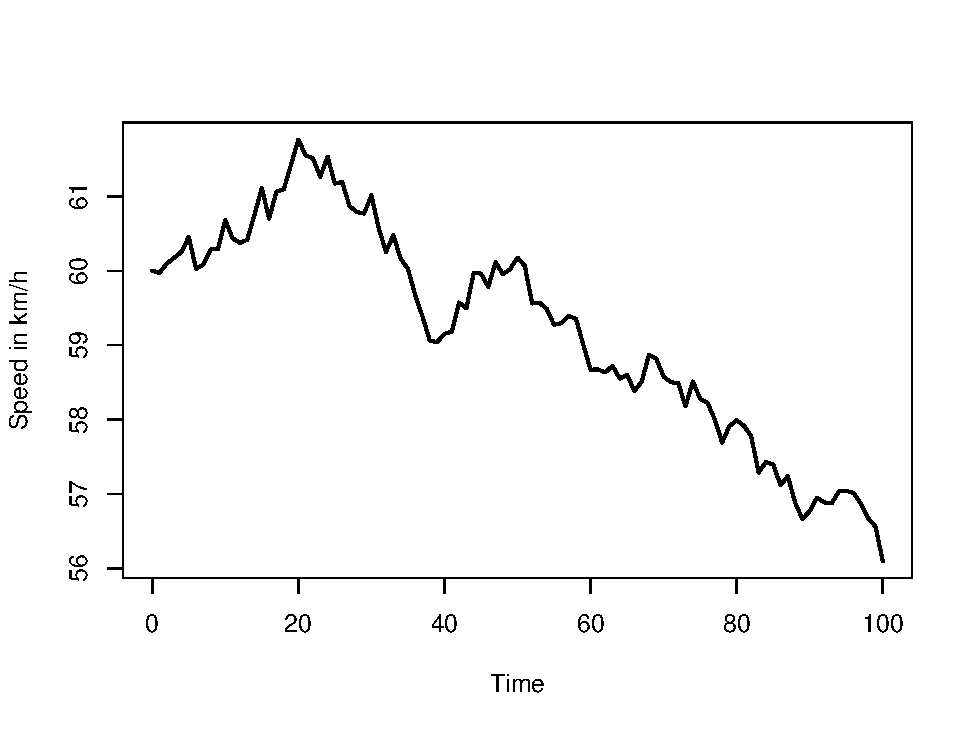
\includegraphics[width=0.8\linewidth]{SimBook_files/figure-latex/fig-cont-1} 

}

\caption{Example of a discrete dynamic simulation}\label{fig:fig-cont}
\end{figure}

In later chapters we will focus on discrete simulations, which are usually called \emph{discrete-event simulation}. Continuous simulations will not be discussed in these notes.

\hypertarget{elements-of-a-simulation-model}{%
\section{Elements of a simulation model}\label{elements-of-a-simulation-model}}

We next introduce some terminology which we will need in the following.

\hypertarget{objects-of-the-model}{%
\subsection{Objects of the model}\label{objects-of-the-model}}

There are two types of objects a simulation model is often made of:

\begin{itemize}
\item
  \emph{Entities}: individual elements of the system that are being simulated and whose behavior is being explicitly tracked. Each entity can be individually identified;
\item
  \emph{Resources}: also individual elements of the system but they are not modelled individually. They are treated as countable items whose behavior is not tracked.
\end{itemize}

Whether an element should be treated as an entity or as a resource is something that the modeller must decide and depends on the purpose of the simulation. Consider our simple donut shop. Clients will be most likely be resources since we are not really interested in what each of them do. Employees may either be considered as entities or resources: in the former case we want to track the amount of time each of them are working; in the latter the model would only be able to output an overview of how busy overall the employees are.

\hypertarget{organization-of-entities-and-resources}{%
\subsection{Organization of entities and resources}\label{organization-of-entities-and-resources}}

\begin{itemize}
\item
  \emph{Attributes}: properties of objects (that is entities and resources). This is often used to control the behavior of the object. In our donut shop an attribute may be the state of an employee: whether she is busy or available. In a more comprehensive simulation, an attribute might be the type of donut a customer will buy (for instance, chocolate, vanilla or jam).
\item
  \emph{State}: collection of variables necessary to describe the system at any time point. In our donut shop, in the simplest case the necessary variables are number of customers queuing and number of busy employees. This fully characterizes the system.
\item
  \emph{List}: collection of entites or resources ordered in some logical fashion. For instance, the customers waiting in our shop may be ordered in the so-called ``fist-come, first-served" scheme, that is customers will be served in the order they arrived in the shop.
\end{itemize}

\hypertarget{operations-of-the-objects}{%
\subsection{Operations of the objects}\label{operations-of-the-objects}}

During a simulation study, entities and resources will cooperate and therefore change state. The following terminology describe this as well as the flow of time:

\begin{itemize}
\item
  \emph{Event}: instant of time where the state of the system changes. In the donut shop suppose that there are currently two customers being served. An event is when a customer has finished being served: the number of busy employees decreases by one and there is one less customer queuing.
\item
  \emph{Activity}: a time period of specified length which is known when it begins (although its length may be random). The time an employee takes to serve a customer is an example of an activity: this may be specified in terms of a random distribution.
\item
  \emph{Delay}: duration of time of unspecified length, which is not known until it ends. This is not specified by the modeller ahead of time but is determined by the conditions of the system. Very often this is one of the desired output of a simulation. For instance, a delay is the waiting time of a customer in the queue of our donut shop.
\item
  \emph{Clock}: variable representing simulated time.
\end{itemize}

\hypertarget{the-donut-shop-example}{%
\section{The donut shop example}\label{the-donut-shop-example}}

Let's consider in more details the donut shop example and let's construct and implement our first simulation model. At this stage, you should not worry about the implementation details. These will be formalized in more details in later chapters.

Let's make some assumptions:

\begin{itemize}
\item
  the queue in the shop is possibly infinite: whenever a customer arrives she will stay in the queue independent of how many customers are already queuing and she will wait until she is served.
\item
  customers are served on a first-come, first-served basis.
\item
  there are two employees. On average they take the same time to serve a customer. Whenever an employee is free, a customer is allocated to that employee. If both employees are free, either of the two starts serving a customer.
\end{itemize}

The components of the simulation model are the following:

\begin{itemize}
\item
  \textbf{System state}: \(N_C(t)\) number of customers waiting to be served at time \(t\); \(N_E(t)\) number of employees busy at time \(t\).
\item
  \textbf{Resources}: customers and employees;
\item
  \textbf{Events}: arrival of a customer; service completion by an employee.
\item
  \textbf{Activities}: time between a customer arrival and the next; service time by an employee.
\item
  \textbf{Delay}: customers' waiting time in the queue until an employee is available.
\end{itemize}

From an abstract point of view we have now defined all components of our simulation model. Before implementing, we need to choose the length of the activities. This is usually done using common sense, intuition or historical data. Suppose for instance that the time between the arrival of customers is modeled as an Exponential distribution with parameter 1/3 (that is on average a customer arrives every three minutes) and the service time is modeled as a continuous Uniform distribution between 1 and 5 (on average a service takes three minutes).

With this information we can now implement the workings of our donut shop. It does not matter the specific code itself, we will learn about it in later chapters. At this stage it is only important to notice that we use the \texttt{simmer} package together with the functionalities of \texttt{magrittr}. We simulate our donut shop for two hours.

\begin{Shaded}
\begin{Highlighting}[]
\FunctionTok{library}\NormalTok{(simmer)}
\FunctionTok{library}\NormalTok{(magrittr)}
\FunctionTok{set.seed}\NormalTok{(}\DecValTok{2021}\NormalTok{)}

\NormalTok{env }\OtherTok{\textless{}{-}}  \FunctionTok{simmer}\NormalTok{(}\StringTok{"donut shop"}\NormalTok{)}

\NormalTok{customer }\OtherTok{\textless{}{-}} \FunctionTok{trajectory}\NormalTok{(}\StringTok{"customer"}\NormalTok{) }\SpecialCharTok{\%\textgreater{}\%} \FunctionTok{seize}\NormalTok{(}\StringTok{"employee"}\NormalTok{, }\DecValTok{1}\NormalTok{) }\SpecialCharTok{\%\textgreater{}\%}
  \FunctionTok{timeout}\NormalTok{(}\ControlFlowTok{function}\NormalTok{() }\FunctionTok{runif}\NormalTok{(}\DecValTok{1}\NormalTok{,}\DecValTok{1}\NormalTok{,}\DecValTok{5}\NormalTok{)) }\SpecialCharTok{\%\textgreater{}\%} \FunctionTok{release}\NormalTok{(}\StringTok{"employee"}\NormalTok{, }\DecValTok{1}\NormalTok{) }

\NormalTok{env }\SpecialCharTok{\%\textgreater{}\%}
  \FunctionTok{add\_resource}\NormalTok{(}\StringTok{"employee"}\NormalTok{, }\DecValTok{2}\NormalTok{) }\SpecialCharTok{\%\textgreater{}\%}
  \FunctionTok{add\_generator}\NormalTok{(}\StringTok{"customer"}\NormalTok{, customer, }\ControlFlowTok{function}\NormalTok{() }\FunctionTok{rexp}\NormalTok{(}\DecValTok{1}\NormalTok{,}\DecValTok{1}\SpecialCharTok{/}\DecValTok{3}\NormalTok{))}

\NormalTok{env }\SpecialCharTok{\%\textgreater{}\%}
  \FunctionTok{run}\NormalTok{(}\AttributeTok{until=}\DecValTok{120}\NormalTok{)}
\end{Highlighting}
\end{Shaded}

The above code creates a simulation of the donut shop for two hours. Next we report some graphical summaries that describe how the system worked.

\begin{Shaded}
\begin{Highlighting}[]
\FunctionTok{library}\NormalTok{(simmer.plot)}
\FunctionTok{library}\NormalTok{(gridExtra)}
\NormalTok{p1 }\OtherTok{\textless{}{-}} \FunctionTok{plot}\NormalTok{(}\FunctionTok{get\_mon\_resources}\NormalTok{(env), }\AttributeTok{metric =} \StringTok{"usage"}\NormalTok{, }\AttributeTok{items =} \StringTok{"server"}\NormalTok{,}\AttributeTok{step =}\NormalTok{ T)}
\NormalTok{p2 }\OtherTok{\textless{}{-}} \FunctionTok{plot}\NormalTok{(}\FunctionTok{get\_mon\_arrivals}\NormalTok{(env), }\AttributeTok{metric =} \StringTok{"waiting\_time"}\NormalTok{)}

\FunctionTok{grid.arrange}\NormalTok{(p1,p2,}\AttributeTok{ncol=}\DecValTok{2}\NormalTok{)}
\end{Highlighting}
\end{Shaded}

\begin{figure}

{\centering 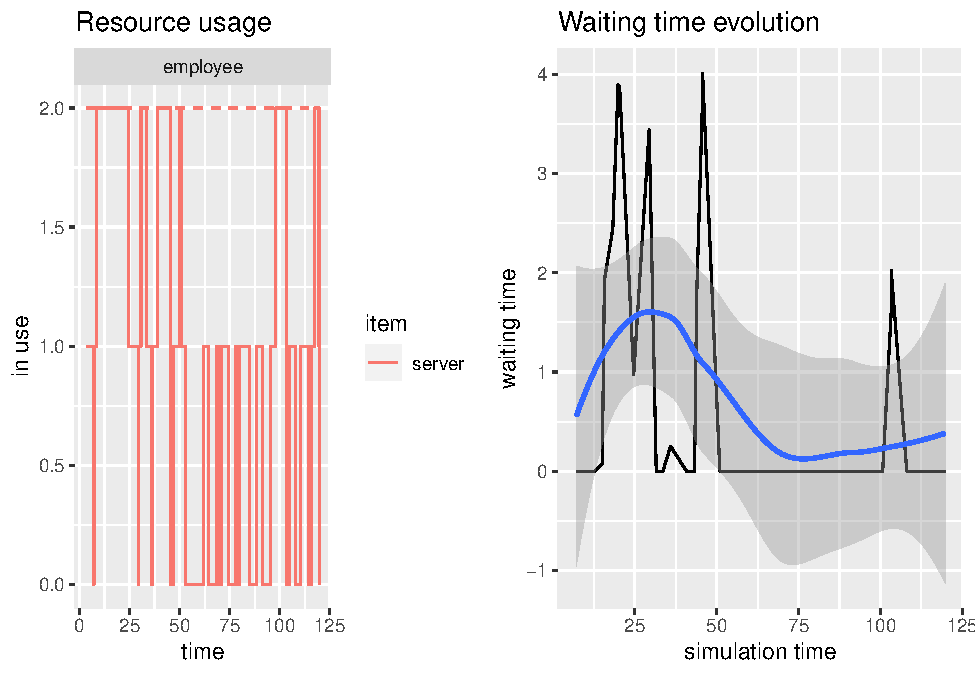
\includegraphics{SimBook_files/figure-latex/donut-1} 

}

\caption{Graphical summaries from the simulation of the donut shop}\label{fig:donut}
\end{figure}

The left plot in Figure 1.3 reports the number of busy employees busy throughout the simulation. We can observe that often no employees were busy, but sometimes both of them are busy. The right plot in Figure 1.3 reports the waiting time of customers throughout the simulation. Most often customers do not wait in our shop and the largest waiting time is of about four minutes.

Some observations:

\begin{itemize}
\item
  this is the result of a single simulation where inputs are random and described by a random variable (for instance, Poisson and Uniform). If we were to run the simulation again we would observe different results.
\item
  given that we have built the simulation model, it is straightforward to change some of the inputs and observe the results under different conditions. For instance, we could investigate what would happen if we had only one employee. We could also investigate the use of different input parameters for the customer arrival times and the service times.
\end{itemize}

\hypertarget{simulating-a-little-health-center}{%
\section{Simulating a little health center}\label{simulating-a-little-health-center}}

Consider now a slightly more complex example where we want to simulate the workings of a little health center. Patients arrive at the health center and are first visited by a nurse. Once they are visited by the nurse they have an actual consultation with a doctor. Once they are finished with the doctor, they meet the administrative staff to schedule a follow-up appointment.

We make the following assumptions:

\begin{itemize}
\item
  as before we assume queues to be infinite and that patients do not leave the health center until they are served by the administrative staff;
\item
  at all steps patients are visited using a first-come, first-served basis
\item
  the health center has one nurse, two doctors and one administrative staff. The two doctors take on average the same time to visit a patient.
\end{itemize}

The components of the simulation model are the following:

\begin{itemize}
\item
  \textbf{System state}:

  \begin{itemize}
  \item
    \(Q_N(t)\): number of patients queuing to see the nurse;
  \item
    \(Q_D(t)\): number of patients queing to see a doctor;
  \item
    \(Q_A(t)\): number of patients queuing to see the staff;
  \item
    \(N_N(t)\): number of nurses available to visit patients;
  \item
    \(N_D(t)\): number of doctors available to visit patients;
  \item
    \(N_A(t)\): number of administrative staff available to visit patients.
  \end{itemize}
\item
  \textbf{Resources}: patients, nurses, doctors and administrative staff;
\item
  \textbf{Events}: arrival of a patient, completion of nurse's visit, completation of doctor's visit, completion of administrative staff's visit.
\item
  \textbf{Activities}: time between the arrival of a patient and the next, visit's times of nurses, doctors and admin staff.
\item
  \textbf{Delay}: customers' waiting time for nurses, doctors and administrative staff
\end{itemize}

We further assume the following activities:

\begin{itemize}
\item
  Nurse visit times follow a Normal distribution with mean 15 and variance 1;
\item
  Doctor visit times follow a Normal distribution with mean 20 and variance 1;
\item
  Administrative staff visit times follow a Normal distribution with mean 5 and variance 1;
\item
  Time between the arrival of patients is modeled as a Normal with mean 10 and variance 4.
\end{itemize}

The model above can be implemented using the following code (we run the simulation for four hours). Again do not worry about it now!

\begin{Shaded}
\begin{Highlighting}[]
\FunctionTok{set.seed}\NormalTok{(}\DecValTok{2021}\NormalTok{)}
\NormalTok{env }\OtherTok{\textless{}{-}} \FunctionTok{simmer}\NormalTok{(}\StringTok{"HealthCenter"}\NormalTok{)}

\NormalTok{patient }\OtherTok{\textless{}{-}} \FunctionTok{trajectory}\NormalTok{(}\StringTok{"patients\textquotesingle{} path"}\NormalTok{) }\SpecialCharTok{\%\textgreater{}\%}
  \FunctionTok{seize}\NormalTok{(}\StringTok{"nurse"}\NormalTok{, }\DecValTok{1}\NormalTok{) }\SpecialCharTok{\%\textgreater{}\%}
  \FunctionTok{timeout}\NormalTok{(}\ControlFlowTok{function}\NormalTok{() }\FunctionTok{rnorm}\NormalTok{(}\DecValTok{1}\NormalTok{, }\DecValTok{15}\NormalTok{)) }\SpecialCharTok{\%\textgreater{}\%}
  \FunctionTok{release}\NormalTok{(}\StringTok{"nurse"}\NormalTok{, }\DecValTok{1}\NormalTok{) }\SpecialCharTok{\%\textgreater{}\%}
  \FunctionTok{seize}\NormalTok{(}\StringTok{"doctor"}\NormalTok{, }\DecValTok{1}\NormalTok{) }\SpecialCharTok{\%\textgreater{}\%}
  \FunctionTok{timeout}\NormalTok{(}\ControlFlowTok{function}\NormalTok{() }\FunctionTok{rnorm}\NormalTok{(}\DecValTok{1}\NormalTok{, }\DecValTok{20}\NormalTok{)) }\SpecialCharTok{\%\textgreater{}\%}
  \FunctionTok{release}\NormalTok{(}\StringTok{"doctor"}\NormalTok{, }\DecValTok{1}\NormalTok{) }\SpecialCharTok{\%\textgreater{}\%}
  \FunctionTok{seize}\NormalTok{(}\StringTok{"administration"}\NormalTok{, }\DecValTok{1}\NormalTok{) }\SpecialCharTok{\%\textgreater{}\%}
  \FunctionTok{timeout}\NormalTok{(}\ControlFlowTok{function}\NormalTok{() }\FunctionTok{rnorm}\NormalTok{(}\DecValTok{1}\NormalTok{, }\DecValTok{5}\NormalTok{)) }\SpecialCharTok{\%\textgreater{}\%}
  \FunctionTok{release}\NormalTok{(}\StringTok{"administration"}\NormalTok{, }\DecValTok{1}\NormalTok{)}

\NormalTok{env }\SpecialCharTok{\%\textgreater{}\%}
  \FunctionTok{add\_resource}\NormalTok{(}\StringTok{"nurse"}\NormalTok{, }\DecValTok{1}\NormalTok{) }\SpecialCharTok{\%\textgreater{}\%}
  \FunctionTok{add\_resource}\NormalTok{(}\StringTok{"doctor"}\NormalTok{, }\DecValTok{2}\NormalTok{) }\SpecialCharTok{\%\textgreater{}\%}
  \FunctionTok{add\_resource}\NormalTok{(}\StringTok{"administration"}\NormalTok{, }\DecValTok{1}\NormalTok{) }\SpecialCharTok{\%\textgreater{}\%}
  \FunctionTok{add\_generator}\NormalTok{(}\StringTok{"patient"}\NormalTok{, patient, }\ControlFlowTok{function}\NormalTok{() }\FunctionTok{rnorm}\NormalTok{(}\DecValTok{1}\NormalTok{, }\DecValTok{10}\NormalTok{, }\DecValTok{2}\NormalTok{))}

\NormalTok{env }\SpecialCharTok{\%\textgreater{}\%} \FunctionTok{run}\NormalTok{(}\DecValTok{240}\NormalTok{)}
\end{Highlighting}
\end{Shaded}

Let's look at some summary statistics.

\begin{Shaded}
\begin{Highlighting}[]
\FunctionTok{plot}\NormalTok{(}\FunctionTok{get\_mon\_resources}\NormalTok{(env), }\AttributeTok{metric =} \StringTok{"utilization"}\NormalTok{)}
\end{Highlighting}
\end{Shaded}

\begin{figure}

{\centering 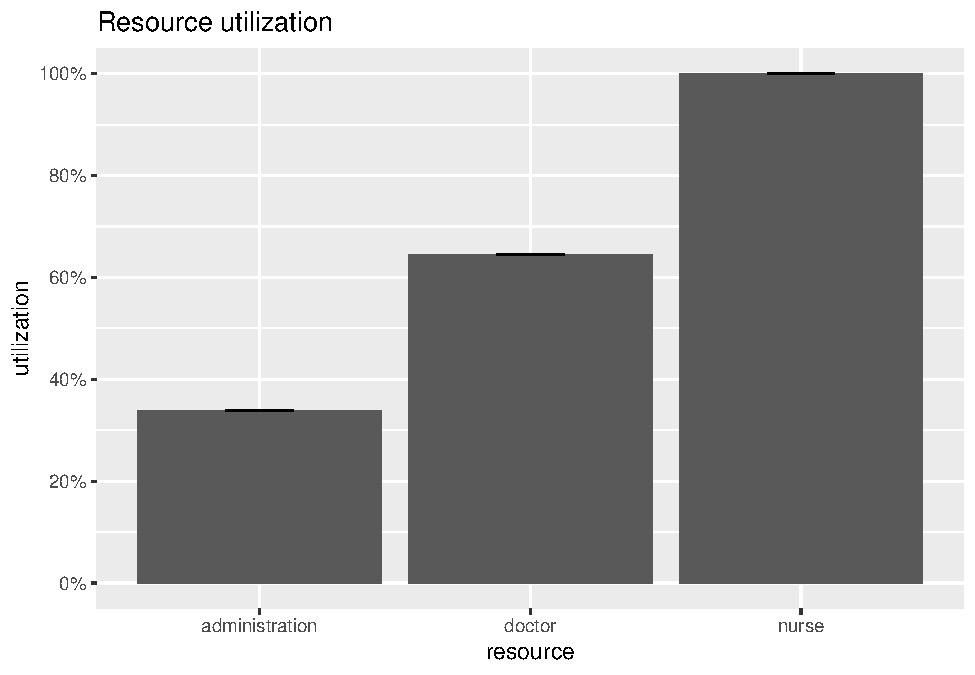
\includegraphics{SimBook_files/figure-latex/unnamed-chunk-4-1} 

}

\caption{Utilization of the resources in the health center}\label{fig:unnamed-chunk-4}
\end{figure}

Figure 1.4 shows the utilization of the different resources in the system. Nurses are most busy, doctors are overall fairly available, whilst the administration is more than half of the time available.

\begin{Shaded}
\begin{Highlighting}[]
\FunctionTok{plot}\NormalTok{(}\FunctionTok{get\_mon\_resources}\NormalTok{(env), }\AttributeTok{metric =} \StringTok{"usage"}\NormalTok{, }\AttributeTok{item =} \StringTok{"server"}\NormalTok{)}
\end{Highlighting}
\end{Shaded}

\begin{figure}

{\centering 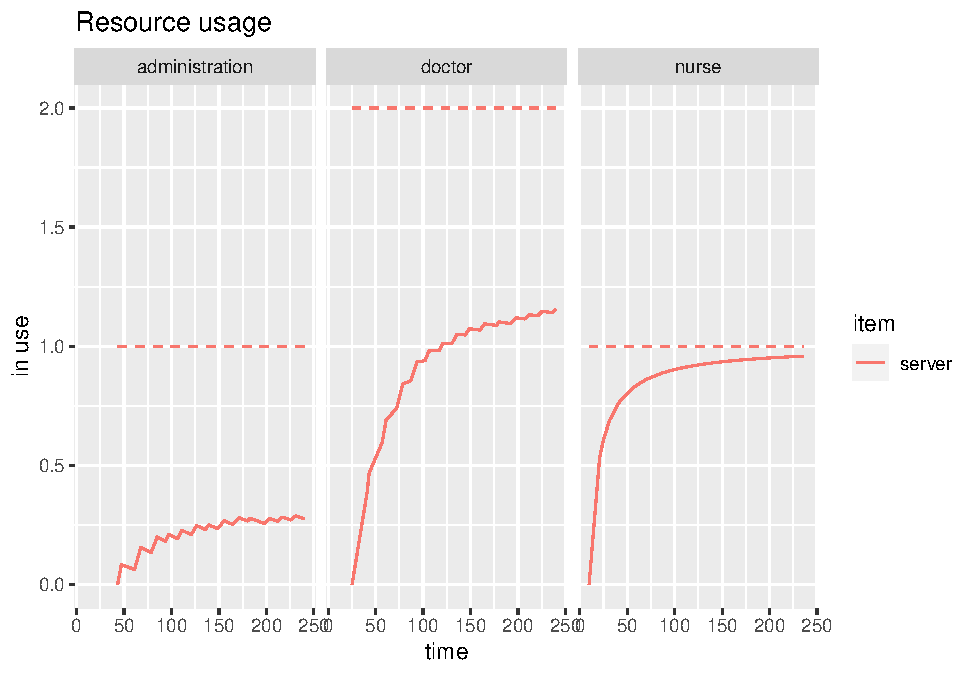
\includegraphics{SimBook_files/figure-latex/unnamed-chunk-5-1} 

}

\caption{Usage of the resources in the health center}\label{fig:unnamed-chunk-5}
\end{figure}

Figure 1.5 confirms this. We see that the usage of nurses is almost 1, whilst for doctors and administrative staff we are below the number of doctors and staff available.

\begin{Shaded}
\begin{Highlighting}[]
\FunctionTok{plot}\NormalTok{(}\FunctionTok{get\_mon\_arrivals}\NormalTok{(env), }\AttributeTok{metric =} \StringTok{"flow\_time"}\NormalTok{)}
\end{Highlighting}
\end{Shaded}

\begin{figure}

{\centering 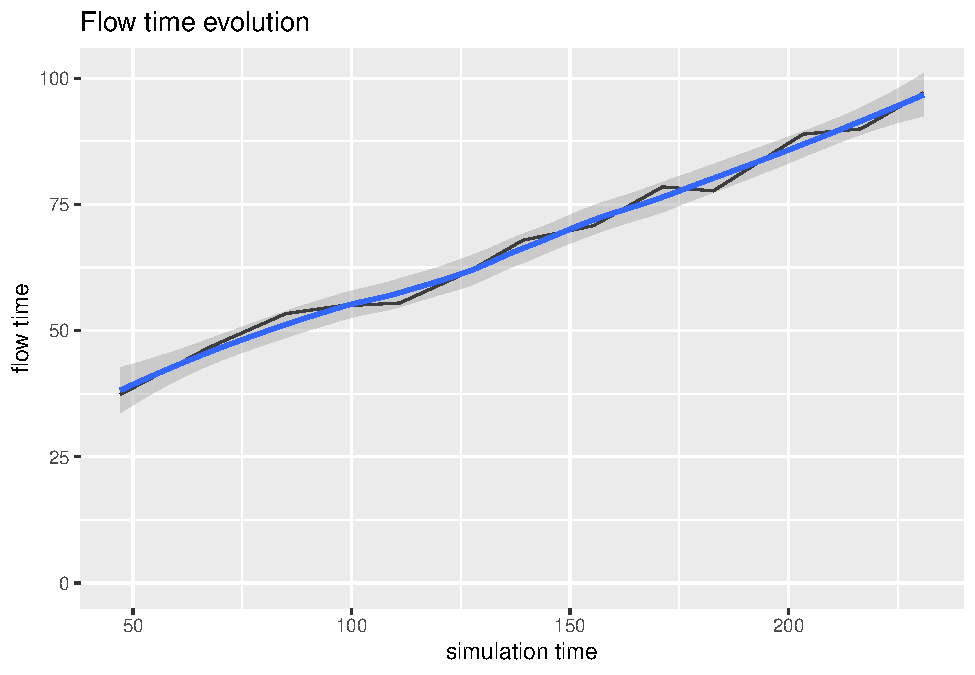
\includegraphics{SimBook_files/figure-latex/unnamed-chunk-6-1} 

}

\caption{Time spent in the health center}\label{fig:unnamed-chunk-6}
\end{figure}

Last Figure 1.6 reports the average time spent by patients in the health center. We can see that as the simulation clock increases, patients spend more time in the health center. From the previous plots, we can deduce that in general patients wait for the nurse, who has been busy all the time during the simulation.

\hypertarget{whats-next}{%
\section{What's next}\label{whats-next}}

The previous examples should have given you an idea of what a simulation model is and what you will be able to implement by the end of the course. However, it will take some time before we get to actually simulate systems. There are various skills that you will need to learn or revise before being able to implement simulation in R yourself. Specifically:

\begin{itemize}
\item
  first we will review the basics of R programming;
\item
  we will then review basic elements of probability and statistics;
\item
  we will discuss how randomness is implemented in programming languages and in R;
\item
  at this stage you will be able to implement your first simple simulations. In particular we will start with static simulation, also called \emph{Monte Carlo} simulation
\item
  we will then look at dynamic simulations as in the previous examples.
\end{itemize}

\hypertarget{r-programming}{%
\chapter{R programming}\label{r-programming}}

R is a programming language most commonly used within the statistical and machine learning community. This chapter will review some of the elements of R programming that will be used in later chapters. Do not expect this chapter to be exhaustive or self-contained. It is intended to give a quick refresh of R for users that have at least some experience with this programming language. There are many topics and concepts which are fundamental but will not be reviewed in this chapter. However, you should aim to master the topics included in this chapter since they will appear again later on in these notes. There are many other resources if you want to have a more in-depth look into R programming.

\begin{itemize}
\item
  The books of Hadley Wickham are surely a great starting point and are all available \href{http://hadley.nz/}{here}.
\item
  If you are unsure on how to do something with R, Google it!!! The community of R users is so wide that surely someone else has already asked your same question.
\item
  The R help is extremely useful and comprehensive. If you want to know more about a function, suppose it is called function, you can type \texttt{?function}.
\end{itemize}

\hypertarget{why-r}{%
\section{Why R?}\label{why-r}}

As mentioned in the previous chapter, simulation is very often applied in many areas, for instance management science and engineering. Often a simulation is carried out using an Excel spreadsheet or using a specialised software whose only purpose is creating simulations. Historically, R has not been at the forefront of the implementation of simulation models, in particular of discrete-event simulations. Only recently, R packages implementing discrete-event simulation have appeared, most importantly the \texttt{simmer} R package that you will learn using in later chapters.

These notes are intended to provide a unique view of simulation with specific implementation in the R programming language. Some of the strenght of R are:

\begin{itemize}
\item
  it is free, open-source and available in all major operating systems;
\item
  the community of R users is huge, with many forums, sites and resources that give you practical support in developing your own code;
\item
  a massive set of add-on packages to increase the capabilities of the basic R environment;
\item
  functions to perform state-of-the-art statistical and machine-learning methods. Researchers sometimes create an associated R package to any article they publish so for others to use their methods;
\item
  the integrated development environment RStudio provides a user-friendly environment to make the R programming experience more pleasing;
\item
  powerful communication tools to create documents and presentations embedding R code and R output. As a matter of fact this very book is created in R!!!!
\end{itemize}

\hypertarget{r-basics}{%
\section{R basics}\label{r-basics}}

So let's get started with R programming!

\hypertarget{r-as-a-calculator}{%
\subsection{R as a calculator}\label{r-as-a-calculator}}

In its most basic usage, we can use R as a calculator. Basic algebraic operations can be carried out as you would expect. The symbol \texttt{+} is for sum, \texttt{-} for subtraction, \texttt{*} for multiplication and \texttt{/} for division. Here are some examples:

\begin{Shaded}
\begin{Highlighting}[]
\DecValTok{4} \SpecialCharTok{+} \DecValTok{2}
\end{Highlighting}
\end{Shaded}

\begin{verbatim}
## [1] 6
\end{verbatim}

\begin{Shaded}
\begin{Highlighting}[]
\DecValTok{4} \SpecialCharTok{{-}} \DecValTok{2}
\end{Highlighting}
\end{Shaded}

\begin{verbatim}
## [1] 2
\end{verbatim}

\begin{Shaded}
\begin{Highlighting}[]
\DecValTok{4} \SpecialCharTok{*} \DecValTok{2}
\end{Highlighting}
\end{Shaded}

\begin{verbatim}
## [1] 8
\end{verbatim}

\begin{Shaded}
\begin{Highlighting}[]
\DecValTok{5} \SpecialCharTok{/} \DecValTok{2}
\end{Highlighting}
\end{Shaded}

\begin{verbatim}
## [1] 2.5
\end{verbatim}

\hypertarget{variable-assignment}{%
\subsection{Variable assignment}\label{variable-assignment}}

In R the symbol \texttt{\textless{}-} is used to assign a quantity to a variable. For instance, \texttt{a\ \textless{}-\ 4} assigns the number \texttt{4} to the variable \texttt{a} and \texttt{b\ \textless{}-\ 3} assigns the number \texttt{3} to \texttt{b}. It is much more common to work with variables in programming. Basic operations can then be performed over variables.

\begin{Shaded}
\begin{Highlighting}[]
\NormalTok{a }\OtherTok{\textless{}{-}} \DecValTok{4}
\NormalTok{b }\OtherTok{\textless{}{-}} \DecValTok{3}
\NormalTok{a }\SpecialCharTok{+}\NormalTok{ b}
\end{Highlighting}
\end{Shaded}

\begin{verbatim}
## [1] 7
\end{verbatim}

\begin{Shaded}
\begin{Highlighting}[]
\NormalTok{a }\SpecialCharTok{{-}}\NormalTok{ b}
\end{Highlighting}
\end{Shaded}

\begin{verbatim}
## [1] 1
\end{verbatim}

Notice for example that the code \texttt{a\ \textless{}-\ 4} does not show us the value of the variable \texttt{a}. It only creates this assignment. If we want to print the value of a variable, we have to explictly type the name of the variable.

\begin{Shaded}
\begin{Highlighting}[]
\NormalTok{a}
\end{Highlighting}
\end{Shaded}

\begin{verbatim}
## [1] 4
\end{verbatim}

\hypertarget{data-types}{%
\subsection{Data types}\label{data-types}}

In the previous examples we worked with numbers, but variables could be assigned other types of information. There are four basic types:

\begin{itemize}
\item
  \emph{Logicals} or \emph{Booleans}: corresponding to \texttt{TRUE} and \texttt{FALSE}, also abbreviated as \texttt{T} and \texttt{F} respectively;
\item
  \emph{Doubles}: real numbers;
\item
  \emph{Characters}: strings of text surrounded by \texttt{"} (for example \texttt{"hi"}) or by \texttt{\textquotesingle{}} (for example `by');
\item
  \emph{Integers}: integer numbers. If you type an integer in R, as before 3 or 4, it will usually be stored as a double unless explicitly defined.
\end{itemize}

Examples:

\begin{Shaded}
\begin{Highlighting}[]
\NormalTok{a }\OtherTok{\textless{}{-}} \ConstantTok{TRUE}
\NormalTok{a}
\end{Highlighting}
\end{Shaded}

\begin{verbatim}
## [1] TRUE
\end{verbatim}

\begin{Shaded}
\begin{Highlighting}[]
\NormalTok{b }\OtherTok{\textless{}{-}} \StringTok{"hello"}
\NormalTok{b}
\end{Highlighting}
\end{Shaded}

\begin{verbatim}
## [1] "hello"
\end{verbatim}

\hypertarget{vectors}{%
\subsection{Vectors}\label{vectors}}

In all previous examples the variables included one element only. More generally we can define sequences of elements or so-called \emph{vectors}. They can be defined with the command \texttt{c}, which stands for combine.

\begin{Shaded}
\begin{Highlighting}[]
\NormalTok{vec }\OtherTok{\textless{}{-}} \FunctionTok{c}\NormalTok{(}\DecValTok{1}\NormalTok{,}\DecValTok{3}\NormalTok{,}\DecValTok{5}\NormalTok{,}\DecValTok{7}\NormalTok{)}
\NormalTok{vec}
\end{Highlighting}
\end{Shaded}

\begin{verbatim}
## [1] 1 3 5 7
\end{verbatim}

So \texttt{vec} includes the sequence of numbers 1, 3, 5, 7. Notice that a vector can only include one data type. Consider the following:

\begin{Shaded}
\begin{Highlighting}[]
\NormalTok{vec }\OtherTok{\textless{}{-}} \FunctionTok{c}\NormalTok{(}\DecValTok{1}\NormalTok{, }\StringTok{"hello"}\NormalTok{, }\ConstantTok{TRUE}\NormalTok{)}
\NormalTok{vec}
\end{Highlighting}
\end{Shaded}

\begin{verbatim}
## [1] "1"     "hello" "TRUE"
\end{verbatim}

We created a variable \texttt{vec} where the first entry is a number, then a character string, then a Boolean. When we print \texttt{vec}, we get that its elements are \texttt{"1"}, \texttt{"hello"} and \texttt{"TRUE"}: it has transformed the number \texttt{1} into the string \texttt{"1"} and the Boolean \texttt{TRUE} into \texttt{"TRUE"}.

\hypertarget{matrices}{%
\subsection{Matrices}\label{matrices}}

Matrices are tables of elements that are organized in rows and columns. You can think of them as an arrangement of vectors into a table. Matrices must have the same data type in all its entries, as for vectors. Matrices can be constructed in multiple ways. One way is by stacking vectors into a matrix row-by-row with the command \texttt{rbind}. Consider the following example.

\begin{Shaded}
\begin{Highlighting}[]
\NormalTok{row1 }\OtherTok{\textless{}{-}} \FunctionTok{c}\NormalTok{(}\DecValTok{1}\NormalTok{,}\DecValTok{2}\NormalTok{,}\DecValTok{3}\NormalTok{)}
\NormalTok{row2 }\OtherTok{\textless{}{-}} \FunctionTok{c}\NormalTok{(}\DecValTok{4}\NormalTok{,}\DecValTok{5}\NormalTok{,}\DecValTok{6}\NormalTok{)}
\NormalTok{row3 }\OtherTok{\textless{}{-}} \FunctionTok{c}\NormalTok{(}\DecValTok{7}\NormalTok{,}\DecValTok{8}\NormalTok{,}\DecValTok{9}\NormalTok{)}
\NormalTok{mat }\OtherTok{\textless{}{-}} \FunctionTok{rbind}\NormalTok{(row1,row2,row3)}
\NormalTok{mat}
\end{Highlighting}
\end{Shaded}

\begin{verbatim}
##      [,1] [,2] [,3]
## row1    1    2    3
## row2    4    5    6
## row3    7    8    9
\end{verbatim}

So first we created vectors \texttt{row1\ =\ (1,2,3)}, \texttt{row2\ =\ (4,5,6)} and \texttt{row3\ =\ (7,8,9)} and then organizing them together into the matrix \texttt{mat}.

The following code follows the same procedure but now organizes vectors by columns instead using the command \texttt{cbind}.

\begin{Shaded}
\begin{Highlighting}[]
\NormalTok{col1 }\OtherTok{\textless{}{-}} \FunctionTok{c}\NormalTok{(}\DecValTok{1}\NormalTok{,}\DecValTok{2}\NormalTok{,}\DecValTok{3}\NormalTok{)}
\NormalTok{col2 }\OtherTok{\textless{}{-}} \FunctionTok{c}\NormalTok{(}\DecValTok{4}\NormalTok{,}\DecValTok{5}\NormalTok{,}\DecValTok{6}\NormalTok{)}
\NormalTok{col3 }\OtherTok{\textless{}{-}} \FunctionTok{c}\NormalTok{(}\DecValTok{7}\NormalTok{,}\DecValTok{8}\NormalTok{,}\DecValTok{9}\NormalTok{)}
\NormalTok{mat }\OtherTok{\textless{}{-}} \FunctionTok{cbind}\NormalTok{(col1,col2,col3)}
\NormalTok{mat}
\end{Highlighting}
\end{Shaded}

\begin{verbatim}
##      col1 col2 col3
## [1,]    1    4    7
## [2,]    2    5    8
## [3,]    3    6    9
\end{verbatim}

Last, there is also a command called \texttt{matrix} to create a matrix. It takes a vector, defined using the command \texttt{c} and stores its entries into a matrix of \texttt{nrow} rows and \texttt{ncol} columns. Consider the following example.

\begin{Shaded}
\begin{Highlighting}[]
\NormalTok{vec }\OtherTok{\textless{}{-}} \FunctionTok{c}\NormalTok{(}\DecValTok{1}\NormalTok{,}\DecValTok{2}\NormalTok{,}\DecValTok{3}\NormalTok{,}\DecValTok{4}\NormalTok{,}\DecValTok{5}\NormalTok{,}\DecValTok{6}\NormalTok{,}\DecValTok{7}\NormalTok{,}\DecValTok{8}\NormalTok{,}\DecValTok{9}\NormalTok{)}
\NormalTok{mat }\OtherTok{\textless{}{-}} \FunctionTok{matrix}\NormalTok{(vec, }\AttributeTok{nrow =} \DecValTok{3}\NormalTok{, }\AttributeTok{ncol =} \DecValTok{3}\NormalTok{)}
\NormalTok{mat}
\end{Highlighting}
\end{Shaded}

\begin{verbatim}
##      [,1] [,2] [,3]
## [1,]    1    4    7
## [2,]    2    5    8
## [3,]    3    6    9
\end{verbatim}

So first we created a vector \texttt{vec} with numbers from 1 to 9 and then stored them in a matrix with 3 rows and 3 columns. Number are stored by column: the first element of \texttt{vec} is in entry (1,1), the second element of \texttt{vec} is in entry (2,1), and so on.

\hypertarget{dataframes}{%
\subsection{Dataframes}\label{dataframes}}

Dataframes are very similar as matrices, they are tables organized in rows and columns. However, different to matrices they can have columns with different data types. They can be created with the command \texttt{data.frame}.

\begin{Shaded}
\begin{Highlighting}[]
\NormalTok{data }\OtherTok{\textless{}{-}} \FunctionTok{data.frame}\NormalTok{(}\AttributeTok{X1 =} \FunctionTok{c}\NormalTok{(}\DecValTok{1}\NormalTok{,}\DecValTok{2}\NormalTok{,}\DecValTok{3}\NormalTok{), }\AttributeTok{X2 =} \FunctionTok{c}\NormalTok{(}\ConstantTok{TRUE}\NormalTok{,}\ConstantTok{FALSE}\NormalTok{,}\ConstantTok{FALSE}\NormalTok{),}
                   \AttributeTok{X3 =} \FunctionTok{c}\NormalTok{(}\StringTok{"male"}\NormalTok{,}\StringTok{"male"}\NormalTok{,}\StringTok{"female"}\NormalTok{))}
\NormalTok{data}
\end{Highlighting}
\end{Shaded}

\begin{verbatim}
##   X1    X2     X3
## 1  1  TRUE   male
## 2  2 FALSE   male
## 3  3 FALSE female
\end{verbatim}

The dataframe \texttt{data} includes three columns: the first column \texttt{X1} of numbers, the second column \texttt{X2} of Boolean and the third column \texttt{X3} of characters. Dataframes are the objects that are most commonly used in real world data analysis.

\hypertarget{null-and-na}{%
\subsection{\texorpdfstring{\texttt{NULL} and \texttt{NA}}{NULL and NA}}\label{null-and-na}}

The expression \texttt{NA} is used in R to denote a missing value. Consider the following example.

\begin{Shaded}
\begin{Highlighting}[]
\NormalTok{vec }\OtherTok{\textless{}{-}} \FunctionTok{c}\NormalTok{(}\DecValTok{3}\NormalTok{, }\ConstantTok{NA}\NormalTok{, }\DecValTok{5}\NormalTok{)}
\NormalTok{vec}
\end{Highlighting}
\end{Shaded}

\begin{verbatim}
## [1]  3 NA  5
\end{verbatim}

Although the second element of \texttt{vec} is the expression \texttt{NA}, R recognizes that it is used for missing value and therefore the elements 3 and 5 are still considered numbers: indeed they are not printed as \texttt{"3"} and \texttt{"5"}.

\texttt{NULL} is an additional datatype. This can have various uses. For instance, it is associated to a vector with no entries.

\begin{Shaded}
\begin{Highlighting}[]
\FunctionTok{c}\NormalTok{()}
\end{Highlighting}
\end{Shaded}

\begin{verbatim}
## NULL
\end{verbatim}

\hypertarget{accessing-and-manipulating-variables}{%
\section{Accessing and manipulating variables}\label{accessing-and-manipulating-variables}}

Now that we have described the main objects we will work with in R, we can discuss how to access specific information.

\hypertarget{accessing-a-single-element}{%
\subsection{Accessing a single element}\label{accessing-a-single-element}}

Given a vector \texttt{vec} we can access its i-th entry with \texttt{vec{[}i{]}}.

\begin{Shaded}
\begin{Highlighting}[]
\NormalTok{vec }\OtherTok{\textless{}{-}} \FunctionTok{c}\NormalTok{(}\DecValTok{1}\NormalTok{,}\DecValTok{3}\NormalTok{,}\DecValTok{5}\NormalTok{)}
\NormalTok{vec[}\DecValTok{2}\NormalTok{]}
\end{Highlighting}
\end{Shaded}

\begin{verbatim}
## [1] 3
\end{verbatim}

For a matrix or a dataframe we need to specify the associated row and column. If we have a matrix \texttt{mat} we can access the element in entry (i,j) with \texttt{mat{[}i,j{]}}.

\begin{Shaded}
\begin{Highlighting}[]
\NormalTok{mat }\OtherTok{\textless{}{-}} \FunctionTok{matrix}\NormalTok{(}\FunctionTok{c}\NormalTok{(}\DecValTok{1}\NormalTok{,}\DecValTok{2}\NormalTok{,}\DecValTok{3}\NormalTok{,}\DecValTok{4}\NormalTok{,}\DecValTok{5}\NormalTok{,}\DecValTok{6}\NormalTok{,}\DecValTok{7}\NormalTok{,}\DecValTok{8}\NormalTok{,}\DecValTok{9}\NormalTok{), }\AttributeTok{ncol=}\DecValTok{3}\NormalTok{, }\AttributeTok{nrow =}\DecValTok{3}\NormalTok{)}
\NormalTok{mat[}\DecValTok{1}\NormalTok{,}\DecValTok{3}\NormalTok{]}
\end{Highlighting}
\end{Shaded}

\begin{verbatim}
## [1] 7
\end{verbatim}

\hypertarget{acessing-multiple-entries}{%
\subsection{Acessing multiple entries}\label{acessing-multiple-entries}}

To access multiple entries we can on the other hand define a vector of indexes of the elements we want to access. Consider the following examples:

\begin{Shaded}
\begin{Highlighting}[]
\NormalTok{vec }\OtherTok{\textless{}{-}} \FunctionTok{c}\NormalTok{(}\DecValTok{1}\NormalTok{,}\DecValTok{3}\NormalTok{,}\DecValTok{5}\NormalTok{)}
\NormalTok{vec[}\FunctionTok{c}\NormalTok{(}\DecValTok{1}\NormalTok{,}\DecValTok{2}\NormalTok{)]}
\end{Highlighting}
\end{Shaded}

\begin{verbatim}
## [1] 1 3
\end{verbatim}

The above code accesses the first two entries of the vector \texttt{vec}. To do this we had to define a vector using \texttt{c(1,2)} stating the entries we wanted to look at. For matrices consider:

\begin{Shaded}
\begin{Highlighting}[]
\NormalTok{mat }\OtherTok{\textless{}{-}} \FunctionTok{matrix}\NormalTok{(}\FunctionTok{c}\NormalTok{(}\DecValTok{1}\NormalTok{,}\DecValTok{2}\NormalTok{,}\DecValTok{3}\NormalTok{,}\DecValTok{4}\NormalTok{,}\DecValTok{5}\NormalTok{,}\DecValTok{6}\NormalTok{,}\DecValTok{7}\NormalTok{,}\DecValTok{8}\NormalTok{,}\DecValTok{9}\NormalTok{), }\AttributeTok{ncol=}\DecValTok{3}\NormalTok{, }\AttributeTok{nrow =}\DecValTok{3}\NormalTok{)}
\NormalTok{mat[}\FunctionTok{c}\NormalTok{(}\DecValTok{1}\NormalTok{,}\DecValTok{2}\NormalTok{),}\FunctionTok{c}\NormalTok{(}\DecValTok{2}\NormalTok{,}\DecValTok{3}\NormalTok{)]}
\end{Highlighting}
\end{Shaded}

\begin{verbatim}
##      [,1] [,2]
## [1,]    4    7
## [2,]    5    8
\end{verbatim}

The syntax is very similar as before. We defined to index vectors, one for the rows and one for columns. The two statements \texttt{c(1,2)} and \texttt{c(2,3)} are separated by a comma to denote that the first selects the first and second row, whilst the second selects the second and third column.

If one wants to access full rows or full columns, the argument associated to rows or columns is left blank. Consider the following examples.

\begin{Shaded}
\begin{Highlighting}[]
\NormalTok{mat }\OtherTok{\textless{}{-}} \FunctionTok{matrix}\NormalTok{(}\FunctionTok{c}\NormalTok{(}\DecValTok{1}\NormalTok{,}\DecValTok{2}\NormalTok{,}\DecValTok{3}\NormalTok{,}\DecValTok{4}\NormalTok{,}\DecValTok{5}\NormalTok{,}\DecValTok{6}\NormalTok{,}\DecValTok{7}\NormalTok{,}\DecValTok{8}\NormalTok{,}\DecValTok{9}\NormalTok{), }\AttributeTok{ncol=}\DecValTok{3}\NormalTok{, }\AttributeTok{nrow =}\DecValTok{3}\NormalTok{)}
\NormalTok{mat[}\DecValTok{1}\NormalTok{,]}
\end{Highlighting}
\end{Shaded}

\begin{verbatim}
## [1] 1 4 7
\end{verbatim}

\begin{Shaded}
\begin{Highlighting}[]
\NormalTok{mat[,}\FunctionTok{c}\NormalTok{(}\DecValTok{1}\NormalTok{,}\DecValTok{2}\NormalTok{)]}
\end{Highlighting}
\end{Shaded}

\begin{verbatim}
##      [,1] [,2]
## [1,]    1    4
## [2,]    2    5
## [3,]    3    6
\end{verbatim}

The code \texttt{mat{[}1,{]}} selects the first full row of \texttt{mat}. The code \texttt{mat{[},c(1,2){]}} selects the first and second column of \texttt{mat}. Notice that the comma has always to be included!

To access multiple entries it is often useful to define sequences of number quickly. The following command defines the sequence of integer numbers from 1 to 9.

\begin{Shaded}
\begin{Highlighting}[]
\DecValTok{1}\SpecialCharTok{:}\DecValTok{9}
\end{Highlighting}
\end{Shaded}

\begin{verbatim}
## [1] 1 2 3 4 5 6 7 8 9
\end{verbatim}

More generally, one can define sequences of numbers using \texttt{seq} (see \texttt{?seq}).

\hypertarget{accessing-entries-with-logical-operators}{%
\subsection{Accessing entries with logical operators}\label{accessing-entries-with-logical-operators}}

If we want to access elements of an object based on a condition it is often easier to use logical operators. This means comparing entries using the comparisons you would usually use in mathematical reasoning, for instance being equal to, or being larger to. The syntax is as follows:

\begin{itemize}
\item
  \texttt{==} to check equality (notice the two equal signs)
\item
  \texttt{!=} to check non-equality
\item
  \texttt{\textgreater{}} bigger to
\item
  \texttt{\textgreater{}=} bigger or equal to
\item
  \texttt{\textless{}} less to
\item
  \texttt{\textless{}=} less or equal to
\end{itemize}

Let's see some examples.

\begin{Shaded}
\begin{Highlighting}[]
\NormalTok{vec }\OtherTok{\textless{}{-}} \FunctionTok{c}\NormalTok{(}\DecValTok{2}\NormalTok{,}\DecValTok{3}\NormalTok{,}\DecValTok{4}\NormalTok{,}\DecValTok{5}\NormalTok{,}\DecValTok{6}\NormalTok{)}
\NormalTok{vec }\SpecialCharTok{\textgreater{}} \DecValTok{4}
\end{Highlighting}
\end{Shaded}

\begin{verbatim}
## [1] FALSE FALSE FALSE  TRUE  TRUE
\end{verbatim}

We constructed a vector \texttt{vec} and check which entries were larger than 4. The output is a Boolean vector with the same number of entries as \texttt{vec} where only the last two entries are \texttt{TRUE}. Similarly,

\begin{Shaded}
\begin{Highlighting}[]
\NormalTok{vec }\OtherTok{\textless{}{-}} \FunctionTok{c}\NormalTok{(}\DecValTok{2}\NormalTok{,}\DecValTok{3}\NormalTok{,}\DecValTok{4}\NormalTok{,}\DecValTok{5}\NormalTok{,}\DecValTok{6}\NormalTok{)}
\NormalTok{vec }\SpecialCharTok{==} \DecValTok{4}
\end{Highlighting}
\end{Shaded}

\begin{verbatim}
## [1] FALSE FALSE  TRUE FALSE FALSE
\end{verbatim}

has a \texttt{TRUE} in the third entry only.

So if we were to be interested in returning the elements of \texttt{vec} that are larger than 4 we could use the code

\begin{Shaded}
\begin{Highlighting}[]
\NormalTok{vec }\OtherTok{\textless{}{-}} \FunctionTok{c}\NormalTok{(}\DecValTok{2}\NormalTok{,}\DecValTok{3}\NormalTok{,}\DecValTok{4}\NormalTok{,}\DecValTok{5}\NormalTok{,}\DecValTok{6}\NormalTok{)}
\NormalTok{vec[vec }\SpecialCharTok{\textgreater{}} \DecValTok{4}\NormalTok{]}
\end{Highlighting}
\end{Shaded}

\begin{verbatim}
## [1] 5 6
\end{verbatim}

So we have a vector with only elements 5 and 6.

\hypertarget{manipulating-dataframes}{%
\subsection{Manipulating dataframes}\label{manipulating-dataframes}}

We have seen in the previous section that dataframes are special types of matrices where columns can include a different data type. For this reason they have special way to manipulate and access their entries.

First, specific columns of a dataframe can be accessed using its name and the \texttt{\$} sign as follows.

\begin{Shaded}
\begin{Highlighting}[]
\NormalTok{data }\OtherTok{\textless{}{-}} \FunctionTok{data.frame}\NormalTok{(}\AttributeTok{X1 =} \FunctionTok{c}\NormalTok{(}\DecValTok{1}\NormalTok{,}\DecValTok{2}\NormalTok{,}\DecValTok{3}\NormalTok{), }\AttributeTok{X2 =} \FunctionTok{c}\NormalTok{(}\ConstantTok{TRUE}\NormalTok{,}\ConstantTok{FALSE}\NormalTok{,}\ConstantTok{FALSE}\NormalTok{),}
                   \AttributeTok{X3 =} \FunctionTok{c}\NormalTok{(}\StringTok{"male"}\NormalTok{,}\StringTok{"male"}\NormalTok{,}\StringTok{"female"}\NormalTok{))}
\NormalTok{data}\SpecialCharTok{$}\NormalTok{X1}
\end{Highlighting}
\end{Shaded}

\begin{verbatim}
## [1] 1 2 3
\end{verbatim}

\begin{Shaded}
\begin{Highlighting}[]
\NormalTok{data}\SpecialCharTok{$}\NormalTok{X3}
\end{Highlighting}
\end{Shaded}

\begin{verbatim}
## [1] male   male   female
## Levels: female male
\end{verbatim}

So using the name of the dataframe \texttt{data} followed by \texttt{\$} and then the name of the column, for instance \texttt{X1}, we access that specific column of the dataframe.

Second, we can use the \texttt{\$} sign to add new columns to a dataframe. Consider the following code.

\begin{Shaded}
\begin{Highlighting}[]
\NormalTok{data }\OtherTok{\textless{}{-}} \FunctionTok{data.frame}\NormalTok{(}\AttributeTok{X1 =} \FunctionTok{c}\NormalTok{(}\DecValTok{1}\NormalTok{,}\DecValTok{2}\NormalTok{,}\DecValTok{3}\NormalTok{), }\AttributeTok{X2 =} \FunctionTok{c}\NormalTok{(}\ConstantTok{TRUE}\NormalTok{,}\ConstantTok{FALSE}\NormalTok{,}\ConstantTok{FALSE}\NormalTok{),}
                   \AttributeTok{X3 =} \FunctionTok{c}\NormalTok{(}\StringTok{"male"}\NormalTok{,}\StringTok{"male"}\NormalTok{,}\StringTok{"female"}\NormalTok{))}
\NormalTok{data}\SpecialCharTok{$}\NormalTok{X4 }\OtherTok{\textless{}{-}} \FunctionTok{c}\NormalTok{(}\StringTok{"yes"}\NormalTok{,}\StringTok{"no"}\NormalTok{,}\StringTok{"no"}\NormalTok{)}
\NormalTok{data}
\end{Highlighting}
\end{Shaded}

\begin{verbatim}
##   X1    X2     X3  X4
## 1  1  TRUE   male yes
## 2  2 FALSE   male  no
## 3  3 FALSE female  no
\end{verbatim}

\texttt{data} now includes a fourth column called \texttt{X4} coinciding to the vector \texttt{c("yes","no","no")}.

Third, we can select specific rows of a dataframe using the command \texttt{subset}. Consider the following example.

\begin{Shaded}
\begin{Highlighting}[]
\NormalTok{data }\OtherTok{\textless{}{-}} \FunctionTok{data.frame}\NormalTok{(}\AttributeTok{X1 =} \FunctionTok{c}\NormalTok{(}\DecValTok{1}\NormalTok{,}\DecValTok{2}\NormalTok{,}\DecValTok{3}\NormalTok{), }\AttributeTok{X2 =} \FunctionTok{c}\NormalTok{(}\ConstantTok{TRUE}\NormalTok{,}\ConstantTok{FALSE}\NormalTok{,}\ConstantTok{FALSE}\NormalTok{),}
                   \AttributeTok{X3 =} \FunctionTok{c}\NormalTok{(}\StringTok{"male"}\NormalTok{,}\StringTok{"male"}\NormalTok{,}\StringTok{"female"}\NormalTok{))}
\FunctionTok{subset}\NormalTok{(data, X1 }\SpecialCharTok{\textless{}=} \DecValTok{2}\NormalTok{)}
\end{Highlighting}
\end{Shaded}

\begin{verbatim}
##   X1    X2   X3
## 1  1  TRUE male
## 2  2 FALSE male
\end{verbatim}

The above code returns the rows of \texttt{data} such that \texttt{X1} is less or equal to 2. More complex rules to subset a dataframe can be combined using the and operator \texttt{\&} and the or operator \texttt{\textbar{}}. Let's see an example.

\begin{Shaded}
\begin{Highlighting}[]
\NormalTok{data }\OtherTok{\textless{}{-}} \FunctionTok{data.frame}\NormalTok{(}\AttributeTok{X1 =} \FunctionTok{c}\NormalTok{(}\DecValTok{1}\NormalTok{,}\DecValTok{2}\NormalTok{,}\DecValTok{3}\NormalTok{), }\AttributeTok{X2 =} \FunctionTok{c}\NormalTok{(}\ConstantTok{TRUE}\NormalTok{,}\ConstantTok{FALSE}\NormalTok{,}\ConstantTok{FALSE}\NormalTok{),}
                   \AttributeTok{X3 =} \FunctionTok{c}\NormalTok{(}\StringTok{"male"}\NormalTok{,}\StringTok{"male"}\NormalTok{,}\StringTok{"female"}\NormalTok{))}
\FunctionTok{subset}\NormalTok{(data, X1 }\SpecialCharTok{\textless{}=} \DecValTok{2} \SpecialCharTok{\&}\NormalTok{ X2 }\SpecialCharTok{==} \ConstantTok{TRUE}\NormalTok{)}
\end{Highlighting}
\end{Shaded}

\begin{verbatim}
##   X1   X2   X3
## 1  1 TRUE male
\end{verbatim}

So the above code selects the rows such that \texttt{X1} is less or equal to 2 and \texttt{X2} is \texttt{TRUE}. This is the case only for the first row of \texttt{data}.

\hypertarget{information-about-objects}{%
\subsection{Information about objects}\label{information-about-objects}}

Here is a list of functions which are often useful to get information about objects in R.

\begin{itemize}
\item
  \texttt{length} returns the number of entries in a vector.
\item
  \texttt{dim} returns the number of rows and columns of a matrix or a dataframe
\item
  \texttt{unique} returns the unique elements of a vector or the unique rows of a matrix or a dataframe.
\item
  \texttt{head} returns the first entries of a vector or the first rows of a matrix or a dataframe
\item
  \texttt{order} returns a re-ordering of a vector or a data.frame in ascending order.
\end{itemize}

Let's see some examples.

\begin{Shaded}
\begin{Highlighting}[]
\NormalTok{vec }\OtherTok{\textless{}{-}} \FunctionTok{c}\NormalTok{(}\DecValTok{4}\NormalTok{,}\DecValTok{2}\NormalTok{,}\DecValTok{7}\NormalTok{,}\DecValTok{5}\NormalTok{,}\DecValTok{5}\NormalTok{)}
\FunctionTok{length}\NormalTok{(vec)}
\end{Highlighting}
\end{Shaded}

\begin{verbatim}
## [1] 5
\end{verbatim}

\begin{Shaded}
\begin{Highlighting}[]
\FunctionTok{unique}\NormalTok{(vec)}
\end{Highlighting}
\end{Shaded}

\begin{verbatim}
## [1] 4 2 7 5
\end{verbatim}

\begin{Shaded}
\begin{Highlighting}[]
\FunctionTok{order}\NormalTok{(vec)}
\end{Highlighting}
\end{Shaded}

\begin{verbatim}
## [1] 2 1 4 5 3
\end{verbatim}

\texttt{length} gives the number of elements of \texttt{vec}, \texttt{unique} returns the different values in \texttt{vec} (so 5 is not repeated), \texttt{order} returns in entry i the ordering of the i-th entry of \texttt{vec}. So the first entry of \texttt{order(vec)} is 2 since 4 is the second-smallest entry of \texttt{vec}.

\begin{Shaded}
\begin{Highlighting}[]
\NormalTok{data }\OtherTok{\textless{}{-}} \FunctionTok{data.frame}\NormalTok{(}\AttributeTok{X1 =} \FunctionTok{c}\NormalTok{(}\DecValTok{1}\NormalTok{,}\DecValTok{2}\NormalTok{,}\DecValTok{3}\NormalTok{,}\DecValTok{4}\NormalTok{), }\AttributeTok{X2 =} \FunctionTok{c}\NormalTok{(}\ConstantTok{TRUE}\NormalTok{,}\ConstantTok{FALSE}\NormalTok{,}\ConstantTok{FALSE}\NormalTok{,}\ConstantTok{FALSE}\NormalTok{),}
                   \AttributeTok{X3 =} \FunctionTok{c}\NormalTok{(}\StringTok{"male"}\NormalTok{,}\StringTok{"male"}\NormalTok{,}\StringTok{"female"}\NormalTok{,}\StringTok{"female"}\NormalTok{))}
\FunctionTok{dim}\NormalTok{(data)}
\end{Highlighting}
\end{Shaded}

\begin{verbatim}
## [1] 4 3
\end{verbatim}

So \texttt{dim} tells us that \texttt{data} has four rows and three columns.

\hypertarget{loops-and-conditions}{%
\section{Loops and conditions}\label{loops-and-conditions}}

This section reviews two of the most basic elements of any programming language: \texttt{if} statements and \texttt{cycles} or \texttt{loops}.

\hypertarget{if-statements}{%
\subsection{\texorpdfstring{\texttt{if} statements}{if statements}}\label{if-statements}}

The basic form of an \texttt{if} statement in R is as follows:

\begin{Shaded}
\begin{Highlighting}[]
\ControlFlowTok{if}\NormalTok{(condition)\{true\_action\}}
\end{Highlighting}
\end{Shaded}

Condition must return a Boolean, either \texttt{TRUE} or \texttt{FALSE}. If \texttt{TRUE} then the code follows the code within the curly brackets and performs the \texttt{true\_action}. If \texttt{condition} is \texttt{FALSE} the code does nothing.

It is more customary to also give a chunk of code for the case \texttt{condition} is \texttt{FALSE}. This can be achieved with \texttt{else}.

\begin{Shaded}
\begin{Highlighting}[]
\ControlFlowTok{if}\NormalTok{(condition)\{true\_action\} }\ControlFlowTok{else}\NormalTok{ \{false\_action\}}
\end{Highlighting}
\end{Shaded}

Let's see an example.

\begin{Shaded}
\begin{Highlighting}[]
\NormalTok{a }\OtherTok{\textless{}{-}} \DecValTok{5}
\ControlFlowTok{if}\NormalTok{ (a }\SpecialCharTok{\textless{}} \DecValTok{2}\NormalTok{)\{}\StringTok{"hello"}\NormalTok{\} }\ControlFlowTok{else}\NormalTok{ \{}\StringTok{"goodbye"}\NormalTok{\}}
\end{Highlighting}
\end{Shaded}

\begin{verbatim}
## [1] "goodbye"
\end{verbatim}

The variable \texttt{a} is assigned the number 5. Then we impose a condition: if \texttt{a} is less than 2, we print the text \texttt{"hello"}, otherwise \texttt{"goodbye"} is printed. Since \texttt{a\ \textless{}-\ 5} the code prints correctly \texttt{"goodbye"}. On the other hand if \texttt{a} were assigned \texttt{1}.

\begin{Shaded}
\begin{Highlighting}[]
\NormalTok{a }\OtherTok{\textless{}{-}} \DecValTok{1}
\ControlFlowTok{if}\NormalTok{ (a }\SpecialCharTok{\textless{}} \DecValTok{2}\NormalTok{)\{}\StringTok{"hello"}\NormalTok{\} }\ControlFlowTok{else}\NormalTok{ \{}\StringTok{"goodbye"}\NormalTok{\}}
\end{Highlighting}
\end{Shaded}

\begin{verbatim}
## [1] "hello"
\end{verbatim}

\hypertarget{ifelse}{%
\subsection{\texorpdfstring{\texttt{ifelse}}{ifelse}}\label{ifelse}}

\texttt{if} works when checking a single element and the condition returns either \texttt{TRUE} or \texttt{FALSE}. The command \texttt{ifelse} can be used to quickly check a condition over all elements of a vector. Consider the following example.

\begin{Shaded}
\begin{Highlighting}[]
\NormalTok{vec }\OtherTok{\textless{}{-}} \FunctionTok{c}\NormalTok{(}\DecValTok{1}\NormalTok{, }\DecValTok{3}\NormalTok{, }\DecValTok{5}\NormalTok{, }\DecValTok{7}\NormalTok{, }\DecValTok{9}\NormalTok{)}
\FunctionTok{ifelse}\NormalTok{(vec }\SpecialCharTok{\textgreater{}} \DecValTok{5}\NormalTok{, }\StringTok{"bigger"}\NormalTok{, }\StringTok{"smaller"}\NormalTok{)}
\end{Highlighting}
\end{Shaded}

\begin{verbatim}
## [1] "smaller" "smaller" "smaller" "bigger"  "bigger"
\end{verbatim}

\texttt{vec} contains the values 1, 3, 5, 7, 9 and the \texttt{condition} is if an elemenent of \texttt{vec} is larger than 5. If \texttt{TRUE} the code returns the string \texttt{bigger} and otherwise returns \texttt{smaller}. The code above returns therefore a vector of the same length of \texttt{vec} including either the string \texttt{bigger} or the string \texttt{smaller}.

\hypertarget{loops}{%
\subsection{Loops}\label{loops}}

\texttt{for} loops are used to iterate over items in a vector. They have the following skeleton:

\begin{Shaded}
\begin{Highlighting}[]
\ControlFlowTok{for}\NormalTok{(item }\ControlFlowTok{in}\NormalTok{ vector) \{perform\_action\}}
\end{Highlighting}
\end{Shaded}

For each \texttt{item} in \texttt{vector}, \texttt{perform\_action} is performed once and the value of \texttt{item} is updated each time.

Here is an example.

\begin{Shaded}
\begin{Highlighting}[]
\ControlFlowTok{for}\NormalTok{ (i }\ControlFlowTok{in} \FunctionTok{c}\NormalTok{(}\DecValTok{1}\NormalTok{,}\DecValTok{2}\NormalTok{,}\DecValTok{3}\NormalTok{))\{}
  \FunctionTok{print}\NormalTok{(i)}
\NormalTok{\}}
\end{Highlighting}
\end{Shaded}

\begin{verbatim}
## [1] 1
## [1] 2
## [1] 3
\end{verbatim}

Item is the variable \texttt{i} (it is costumary to use just a letter) and at each step \texttt{i} is set equal to a value in the vector \texttt{c(1,2,3)}. At each of these iterations, the command \texttt{print(i)}, which simply returns the value that \texttt{i} takes is called. Indeed we see that the output is the sequence of numbers 1, 2, 3.

\hypertarget{functions}{%
\section{Functions}\label{functions}}

Functions are chunks of code that are given a name so that they can be easily used multiple times. Perhaps without realising it, you have used functions already many times!

\hypertarget{defining-your-own-function}{%
\subsection{Defining your own function}\label{defining-your-own-function}}

A function is composed of the following elements:

\begin{itemize}
\item
  a name: in R functions are objects just like vectors or matrices and they are given a name.
\item
  arguments: these are objects that will be used within the function.
\item
  body: a chunk of code which is run within the function.
\item
  output: an object that the function returns.
\end{itemize}

Let's consider an example.

\begin{Shaded}
\begin{Highlighting}[]
\NormalTok{my.function }\OtherTok{\textless{}{-}} \ControlFlowTok{function}\NormalTok{(x,y)\{}
\NormalTok{  z }\OtherTok{\textless{}{-}}\NormalTok{ x }\SpecialCharTok{+}\NormalTok{ y}
  \FunctionTok{return}\NormalTok{(z)}
\NormalTok{\}}
\end{Highlighting}
\end{Shaded}

The above function computes the sum of two numbers \texttt{x} and \texttt{y}. Let's call it.

\begin{Shaded}
\begin{Highlighting}[]
\FunctionTok{my.function}\NormalTok{(}\DecValTok{2}\NormalTok{,}\DecValTok{3}\NormalTok{)}
\end{Highlighting}
\end{Shaded}

\begin{verbatim}
## [1] 5
\end{verbatim}

The sum between 2 and 3 is indeed 5.

Let's look at the code line by line. In the first line, we assigned a function using the command \texttt{function} to an object called \texttt{my.function}. \texttt{my.function} has two arguments called \texttt{x} and \texttt{y}. Then there is an opening curly bracket \texttt{\{}. The last line of code has a closing curly bracket \texttt{\}}: whatever is in between the two brackets is a chunk of code which is run when the function is run. The second line computes a new variable called \texttt{z} which stores the sum of \texttt{x} and \texttt{y}. The third line of code tells us that the function should return \texttt{z} as output.

Let's consider a slightly more complicated function.

\begin{Shaded}
\begin{Highlighting}[]
\NormalTok{new.function }\OtherTok{\textless{}{-}} \ControlFlowTok{function}\NormalTok{(x,y)\{}
\NormalTok{  z1 }\OtherTok{\textless{}{-}}\NormalTok{ x}\SpecialCharTok{\^{}}\DecValTok{2}
\NormalTok{  z2 }\OtherTok{\textless{}{-}}\NormalTok{ z1 }\SpecialCharTok{+}\NormalTok{ y}
  \FunctionTok{return}\NormalTok{(z2)}
\NormalTok{\}}
\end{Highlighting}
\end{Shaded}

The \texttt{new.function} returns the sum between the square of the first input \texttt{x} and the second input \texttt{y}. Let's call the function.

\begin{Shaded}
\begin{Highlighting}[]
\FunctionTok{new.function}\NormalTok{(}\DecValTok{2}\NormalTok{,}\DecValTok{3}\NormalTok{)}
\end{Highlighting}
\end{Shaded}

\begin{verbatim}
## [1] 7
\end{verbatim}

\begin{Shaded}
\begin{Highlighting}[]
\FunctionTok{new.function}\NormalTok{(}\DecValTok{3}\NormalTok{,}\DecValTok{2}\NormalTok{)}
\end{Highlighting}
\end{Shaded}

\begin{verbatim}
## [1] 11
\end{verbatim}

Notice that \texttt{new.function(2,3)} is different from \texttt{new.function(3,2)}: indeed in the fist case the sum between 2\^{}2 and 3 is computed, whilst in the second the sum between 3\^{}2 and 2 is computed. Furthermore, that the variable \texttt{z1} exists only within the function: when you call the function the output does not create a variable \texttt{z1}. The output does not create either a variable \texttt{z2} it simply returns the value that is stored in \texttt{z2}, which can the be assigned as in the following example.

\begin{Shaded}
\begin{Highlighting}[]
\NormalTok{value }\OtherTok{\textless{}{-}} \FunctionTok{new.function}\NormalTok{(}\DecValTok{2}\NormalTok{,}\DecValTok{3}\NormalTok{)}
\NormalTok{value}
\end{Highlighting}
\end{Shaded}

\begin{verbatim}
## [1] 7
\end{verbatim}

We stored in \texttt{value} the output of \texttt{new.function(2,3)}.

An equivalent way to write \texttt{new.function} is as follows:

\begin{Shaded}
\begin{Highlighting}[]
\NormalTok{new.function }\OtherTok{\textless{}{-}} \ControlFlowTok{function}\NormalTok{(x,y)\{}
\NormalTok{  x}\SpecialCharTok{\^{}}\DecValTok{2} \SpecialCharTok{+}\NormalTok{ y}
\NormalTok{\}}
\FunctionTok{new.function}\NormalTok{(}\DecValTok{2}\NormalTok{,}\DecValTok{3}\NormalTok{)}
\end{Highlighting}
\end{Shaded}

\begin{verbatim}
## [1] 7
\end{verbatim}

The output is the same. We did not create any variable within the function and we did not explicitly use the \texttt{return} command. R understands that the last line of code is what the function should return.

\hypertarget{calling-functions}{%
\subsection{Calling functions}\label{calling-functions}}

In R functions can be called in various ways. Before we have seen function calls as

\begin{Shaded}
\begin{Highlighting}[]
\FunctionTok{new.function}\NormalTok{(}\DecValTok{2}\NormalTok{,}\DecValTok{3}\NormalTok{)}
\end{Highlighting}
\end{Shaded}

How did it work?

\begin{itemize}
\item
  The function \texttt{new.function} has a first argument \texttt{x} and a second argument \texttt{y}.
\item
  R matched the first argument in \texttt{new.function(2,3)} to \texttt{x}, that is \texttt{x=2}, and the second argument to \texttt{y}, that is \texttt{y=3}.
\end{itemize}

We could have also been more explicit and state what \texttt{x} and \texttt{y} were.

\begin{Shaded}
\begin{Highlighting}[]
\FunctionTok{new.function}\NormalTok{(}\AttributeTok{x=}\DecValTok{2}\NormalTok{, }\AttributeTok{y=}\DecValTok{3}\NormalTok{)}
\end{Highlighting}
\end{Shaded}

\begin{verbatim}
## [1] 7
\end{verbatim}

So now explicitly we state that the input \texttt{x} of \texttt{new.function} is 2 and that the input \texttt{y} is 3. Notice that the two ways of specifying inputs give the exact same results.

\hypertarget{mathematical-and-statistical-functions}{%
\subsection{Mathematical and statistical functions}\label{mathematical-and-statistical-functions}}

The number of functions available in R is massive and it would be impossible to mention them all. Here I just give you a list of mathematical and statistical functions that we may use in the following.

\begin{itemize}
\item
  \texttt{exp} computes the exponential of the entries of an object
\item
  \texttt{log} computes the logarithm of the entries of an object
\item
  \texttt{sqrt} computes the square root of the entries of an
\item
  \texttt{sum} computes the sum of the entries of an object
\item
  \texttt{abs} computes the absolute value of the entries of an object
\item
  \texttt{mean} computes the mean of the entries of an object
\item
  \texttt{sd} computes the standard deviation of the entries of an object
\item
  \texttt{var} computes the variance of the entries of an object
\end{itemize}

\hypertarget{the-apply-family-of-functions}{%
\section{\texorpdfstring{The \texttt{apply} family of functions}{The apply family of functions}}\label{the-apply-family-of-functions}}

One of the biggest limitation of R is that it is slow in performing cycles. For this reason, one should aim at avoiding as much as possible to use of loops.

There are various functions which are designed to help you in avoiding these loops and they are in the family of so called \texttt{apply} functions. There are many of these but we will only see two here.

\hypertarget{the-function-apply}{%
\subsection{\texorpdfstring{The function \texttt{apply}}{The function apply}}\label{the-function-apply}}

Consider the following code.

\begin{Shaded}
\begin{Highlighting}[]
\NormalTok{x }\OtherTok{\textless{}{-}} \FunctionTok{matrix}\NormalTok{(}\FunctionTok{c}\NormalTok{(}\DecValTok{1}\SpecialCharTok{:}\DecValTok{9}\NormalTok{), }\AttributeTok{ncol=}\DecValTok{3}\NormalTok{ , }\AttributeTok{nrow =} \DecValTok{3}\NormalTok{)}
\NormalTok{y }\OtherTok{\textless{}{-}} \FunctionTok{c}\NormalTok{()}
\ControlFlowTok{for}\NormalTok{ (i }\ControlFlowTok{in} \DecValTok{1}\SpecialCharTok{:}\DecValTok{3}\NormalTok{)\{}
\NormalTok{  y[i] }\OtherTok{\textless{}{-}} \FunctionTok{sum}\NormalTok{(x[i,])}
\NormalTok{\}}
\NormalTok{y}
\end{Highlighting}
\end{Shaded}

\begin{verbatim}
## [1] 12 15 18
\end{verbatim}

The code first defines a matrix \texttt{x} and an empty vector \texttt{y} (recall that this is bad practice, but for this example it does not matter). Then there is a \texttt{for} cycle which assigns to the i-th entry of \texttt{y} the sum of the entries of the i-th row of \texttt{x}. So the vector \texttt{y} includes the row-totals.

For this simple example the \texttt{for} cycle is extremely quick, but this is just to illustrate how we can replace it using the \texttt{apply} function.

\begin{Shaded}
\begin{Highlighting}[]
\FunctionTok{apply}\NormalTok{(x, }\DecValTok{1}\NormalTok{, sum)}
\end{Highlighting}
\end{Shaded}

\begin{verbatim}
## [1] 12 15 18
\end{verbatim}

Let's look at the above code. The first input of \texttt{apply} is the object we want to operate upon, in this case the matrix \texttt{x}. The second input specifies if the operation has to act over the rows of the matrix (input equal to 1) or over the columns (input equal to 2). The third input is the operation we want to use, in this case \texttt{sum}.

Beside being faster, the above code is also a lot more compact than using a for loop.

The following example computes the mean of each column of \texttt{x}.

\begin{Shaded}
\begin{Highlighting}[]
\FunctionTok{apply}\NormalTok{(x, }\DecValTok{2}\NormalTok{, mean)}
\end{Highlighting}
\end{Shaded}

\begin{verbatim}
## [1] 2 5 8
\end{verbatim}

\hypertarget{the-function-sapply}{%
\subsection{\texorpdfstring{The function \texttt{sapply}}{The function sapply}}\label{the-function-sapply}}

Consider again our function \texttt{new.function} which computes the sum of the squared of a number \texttt{x} with another number \texttt{y}.

\begin{Shaded}
\begin{Highlighting}[]
\NormalTok{new.function }\OtherTok{\textless{}{-}} \ControlFlowTok{function}\NormalTok{(x,y)\{ x}\SpecialCharTok{\^{}}\DecValTok{2} \SpecialCharTok{+}\NormalTok{ y\}}
\end{Highlighting}
\end{Shaded}

Suppose that we want to compute such a sum for all numbers \texttt{x} from 1 to 10. Suppose that \texttt{y} is chosen as 2. We can achieve this with a \texttt{for} cycle as follows.

\begin{Shaded}
\begin{Highlighting}[]
\NormalTok{x }\OtherTok{\textless{}{-}} \DecValTok{1}\SpecialCharTok{:}\DecValTok{10}
\NormalTok{z }\OtherTok{\textless{}{-}} \FunctionTok{c}\NormalTok{()}
\ControlFlowTok{for}\NormalTok{ (i }\ControlFlowTok{in} \DecValTok{1}\SpecialCharTok{:}\DecValTok{10}\NormalTok{)\{}
\NormalTok{  z[i] }\OtherTok{\textless{}{-}} \FunctionTok{new.function}\NormalTok{(x[i],}\DecValTok{2}\NormalTok{)}
\NormalTok{\}}
\NormalTok{z}
\end{Highlighting}
\end{Shaded}

\begin{verbatim}
##  [1]   3   6  11  18  27  38  51  66  83 102
\end{verbatim}

The function \texttt{sapply} can be used for this specific purpose.

\begin{Shaded}
\begin{Highlighting}[]
\NormalTok{x }\OtherTok{\textless{}{-}} \DecValTok{1}\SpecialCharTok{:}\DecValTok{10}
\FunctionTok{sapply}\NormalTok{(x,new.function, }\AttributeTok{y=}\DecValTok{2}\NormalTok{)}
\end{Highlighting}
\end{Shaded}

\begin{verbatim}
##  [1]   3   6  11  18  27  38  51  66  83 102
\end{verbatim}

The first argument of \texttt{sapply} is a vector of values we want to use as input of a function. The second argument is the function we want to apply multiple times. If the function has more than one input we can then specify what their value is, in this specific case \texttt{y=2}.

Notice that a function can also be defined within \texttt{sapply}.

\begin{Shaded}
\begin{Highlighting}[]
\NormalTok{x }\OtherTok{\textless{}{-}} \DecValTok{1}\SpecialCharTok{:}\DecValTok{10}
\FunctionTok{sapply}\NormalTok{(x, }\ControlFlowTok{function}\NormalTok{(i) i}\SpecialCharTok{\^{}}\DecValTok{2} \SpecialCharTok{+} \DecValTok{2}\NormalTok{)}
\end{Highlighting}
\end{Shaded}

\begin{verbatim}
##  [1]   3   6  11  18  27  38  51  66  83 102
\end{verbatim}

So we defined the vector \texttt{x} and we want to apply the function defined within \texttt{sapply} multiple times: once for each entry in the vector \texttt{x}.

\hypertarget{the-pipe-operator}{%
\section{The pipe operator}\label{the-pipe-operator}}

In practice we often have to call functions in a sequence. Suppose for example you have a vector of numbers. Of those numbers you would like to first compute the absolute value. Then you would like to compute the logarithm of those absolute values. Last you would like to compute the mean of those numbers. In standard R we can write this as

\begin{Shaded}
\begin{Highlighting}[]
\NormalTok{x }\OtherTok{\textless{}{-}} \SpecialCharTok{{-}}\DecValTok{5}\SpecialCharTok{:{-}}\DecValTok{1}
\FunctionTok{mean}\NormalTok{(}\FunctionTok{log}\NormalTok{(}\FunctionTok{abs}\NormalTok{(x)))}
\end{Highlighting}
\end{Shaded}

\begin{verbatim}
## [1] 0.9574983
\end{verbatim}

Such nested code where we apply multiple functions over the same line of code becomes cluttered and difficult to read.

For this reason the package \texttt{magrittr} introduces the so-called pipe operator \texttt{\%\textgreater{}\%} which makes the above code much more readable. Consider the same example using the pipe operator.

\begin{Shaded}
\begin{Highlighting}[]
\FunctionTok{library}\NormalTok{(magrittr)}
\NormalTok{x }\OtherTok{\textless{}{-}} \SpecialCharTok{{-}}\DecValTok{5}\SpecialCharTok{:{-}}\DecValTok{1}
\NormalTok{x }\SpecialCharTok{\%\textgreater{}\%} \FunctionTok{abs}\NormalTok{() }\SpecialCharTok{\%\textgreater{}\%} \FunctionTok{log}\NormalTok{() }\SpecialCharTok{\%\textgreater{}\%} \FunctionTok{mean}\NormalTok{()}
\end{Highlighting}
\end{Shaded}

\begin{verbatim}
## [1] 0.9574983
\end{verbatim}

The above code can be seen as follows: consider the vector \texttt{x} and apply the function \texttt{abs} over its entries. Then apply the function \texttt{log} over the resulting vector and last apply the function \texttt{mean}.

The code is equivalent to standard R but it is simpler to read. So sometimes it is preferrable to code using pipes instead of standard R syntax.

\hypertarget{plotting}{%
\section{Plotting}\label{plotting}}

R has great plotting capabilities. Details about plotting functions and a discussion of when different representations are most appropriate are beyond the scope of these notes. This is just to provide you with a list of functions:

\begin{itemize}
\item
  \texttt{barplot} creates a barplot: notice that you first need to construct a so-called contingency table using the function \texttt{table}.
\item
  \texttt{hist} creates an histogram;
\item
  \texttt{boxplot} creates a boxplot;
\item
  \texttt{plot} creates a scatterplot;
\end{itemize}

There are many functions to customize such plots, and again details can be found in the references given. A package which is often used to create nice data visualization is \texttt{ggplot2}.

\hypertarget{probability-basics}{%
\chapter{Probability Basics}\label{probability-basics}}

Our final aim is to be able to mimic real-world systems as close as possible. In most scenarios we will not know with certainty how things unfold. For instance, we will rarely know the times at which customers enter a shop or the time it will take an employee to complete a task. Let's think again at the donut shop example. The time it takes an employee to serve a costumer depends on the time it takes the customer to specify the order, the number and types of donuts requested, the type of payment etc. To an external observer all these possible causes of variation of serving times appear to be random and due to chance: they cannot be predicted with certainty.

For this reason we will in general assume a probabilistic model for the various components of a simulation. This chapter gives a review of possible models as well as their characteristics.

\hypertarget{discrete-random-variables}{%
\section{Discrete Random Variables}\label{discrete-random-variables}}

We start introducing discrete random variables. Here we will not enter in all the mathematical details and some concepts will be introduced only intuitively. However, some mathematical details will be given for some concepts.

In order to introduce discrete random variables, let's inspect each of the words:

\begin{itemize}
\item
  \emph{variable}: this means that there is some process that takes some value. It is a synonym of function as you have studied in other mathematics classes.
\item
  \emph{random}: this means that the variable takes values according to some probability distribution.
\item
  \emph{discrete}: this refers to the possible values that the variable can take. In this case it is a countable (possibly infinite) set of values.
\end{itemize}

In general we denote a random variable as \(X\) and its possible values as \(\mathbb{X}=\{x_1,x_2,x_3,\dots\}\). The set \(\mathbb{X}\) is called the sample space of \(X\). In real-life we do not know which value in the set \(\mathbb{X}\) the random variable will take.

Let's consider some examples.

\begin{itemize}
\item
  The number of donuts sold in a day in a shop is a discrete random variable which can take values \(\{0,1,2,3,\dots\}\), that is the non-negative integers. In this case the number of possible values is infinite.
\item
  The outcome of a COVID-19 test can be either positive or negative but in advance we do not know which one. So this can be denoted as a discrete random variable taking values in \(\{negative,positive\}\). It is customary to denote the elements of the sample space \(\mathbb{X}\) as numbers. For instance, we could let \(negative = 0\) and \(positive = 1\) and the sample space would be \(\mathbb{X}=\{0,1\}\).
\item
  The number shown on the face of a dice once thrown is a discrete random variable taking values in \(\mathbb{X}=\{1,2,3,4,5,6\}\).
\end{itemize}

\hypertarget{probability-mass-function}{%
\subsection{Probability Mass Function}\label{probability-mass-function}}

The outcome of a discrete random variable is in general unknown, but we want to associate to each outcome, that is to each element of \(\mathbb{X}\), a number describing its likelihood. Such a number is called a probability and it is in general denoted as \(P\).

The \emph{probability mass function} (or pmf) of a random variable \(X\) with sample space \(\mathbb{X}\) is defined as
\[
p(x)=P(X=x), \hspace{1cm} \mbox{for all } x\in\mathbb{X}
\]
So for any outcome \(x\in\mathbb{X}\) the pmf describes the likelihood of that outcome happening.

Recall that pmfs must obey two conditions:

\begin{itemize}
\item
  \(p(x)\geq 0\) for all \(x\in\mathbb{X}\);
\item
  \(\sum_{x\in\mathbb{X}}p(x)=1\).
\end{itemize}

So the pmf associated to each outcome is a non-negative number such that the sum of all these numbers is equal to one.

Let's consider an example at this stage. Suppose a biased dice is thrown such that the numbers 3 and 6 are twice as likely to appear than the other numbers. A pmf describing such a situation is the following:

\begin{longtable}[]{@{}ccccccc@{}}
\toprule
\(x\) & 1 & 2 & 3 & 4 & 5 & 6 \\ \addlinespace
\midrule
\endhead
\(p(x)\) & 1/8 & 1/8 & 2/8 & 1/8 & 1/8 & 2/8 \\ \addlinespace
\bottomrule
\end{longtable}

It is apparent that all numbers \(p(x)\) are non-negative and that their sum is equal to 1: so \(p(x)\) is a pmf. Figure \ref{fig:disc-pmf} gives a graphical visualization of such a pmf.

\begin{figure}
\centering
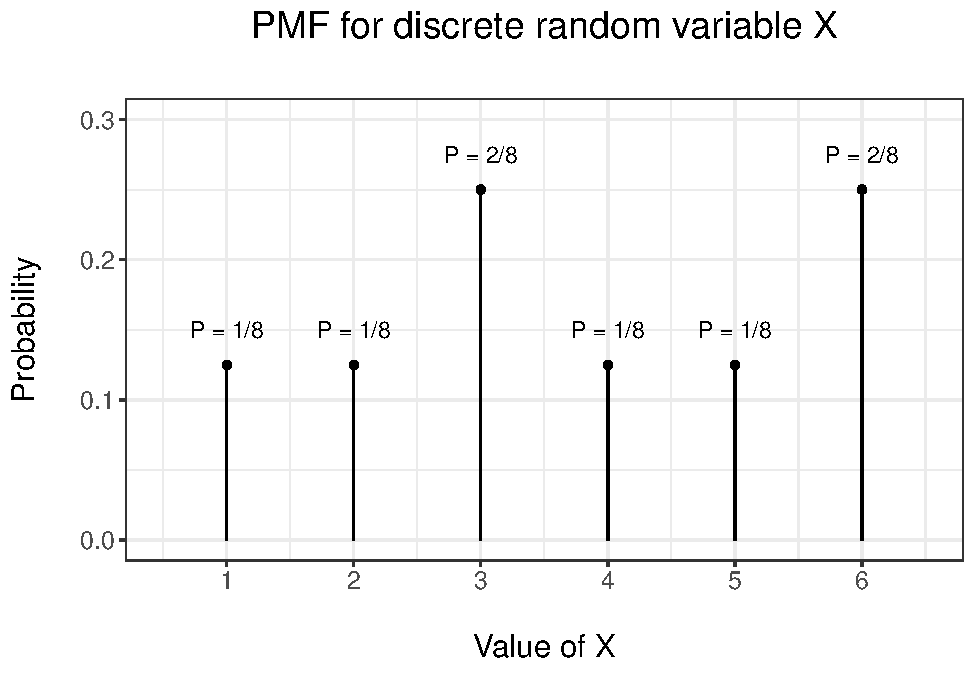
\includegraphics{SimBook_files/figure-latex/disc-pmf-1.pdf}
\caption{\label{fig:disc-pmf}PMF for the biased dice example}
\end{figure}

\hypertarget{cumulative-distribution-function}{%
\subsection{Cumulative Distribution Function}\label{cumulative-distribution-function}}

Whilst you should have been already familiar with the concept of pmf, the next concept may appear to be new. However, you have actually used it multiple times when computing Normal probabilities with the tables.

We now define what is usually called the \emph{cumulative distribution function} (or cdf) of a random variable \(X\). The cdf of \(X\) at the point \(x\in\mathbb{X}\) is
\[
F(x) = P(X \leq x) = \sum_{y \leq x} p(y)
\]
that is the probability that \(X\) is less or equal to \(x\) or equally the sum of the pmf of \(X\) for all values less than \(x\).

Let's consider the dice example to illustrate the idea of cdf and consider the following values \(x\):

\begin{itemize}
\item
  \(x=0\): we compute \(F(0) = P(X\leq 0 )= 0\) since \(X\) cannot take any values less or equal than zero;
\item
  \(x= 0.9\): we compute \(F(0.9)= P(X\leq 0.9) = 0\) using the same reasoning as before;
\item
  \(x = 1\): we compute \(F(1)= P(X\leq 1) = P(X=1) = 1/8\) since \(X\) can take the value 1 with probability 1/8;
\item
  \(x = 1.5\): we compute \(F(1.5) = P(X\leq 1.5) = P(X=1) = 1/8\) using the same reasoning as before;
\item
  \(x = 3.2\): we compute \(F(3.2)=P(X\leq 3.2)=P(X=1)+ P(X=2) + P(X=3)=1/8 + 1/8 + 2/8 = 0.5\) since \(X\) can take the values 1, 2 and 3 which are less than 3.2;
\end{itemize}

We can compute in a similar way the cdf for any value \(x\). A graphical visualization of the resulting CDF is given in Figure \ref{fig:disc-cdf}.

\begin{figure}
\centering
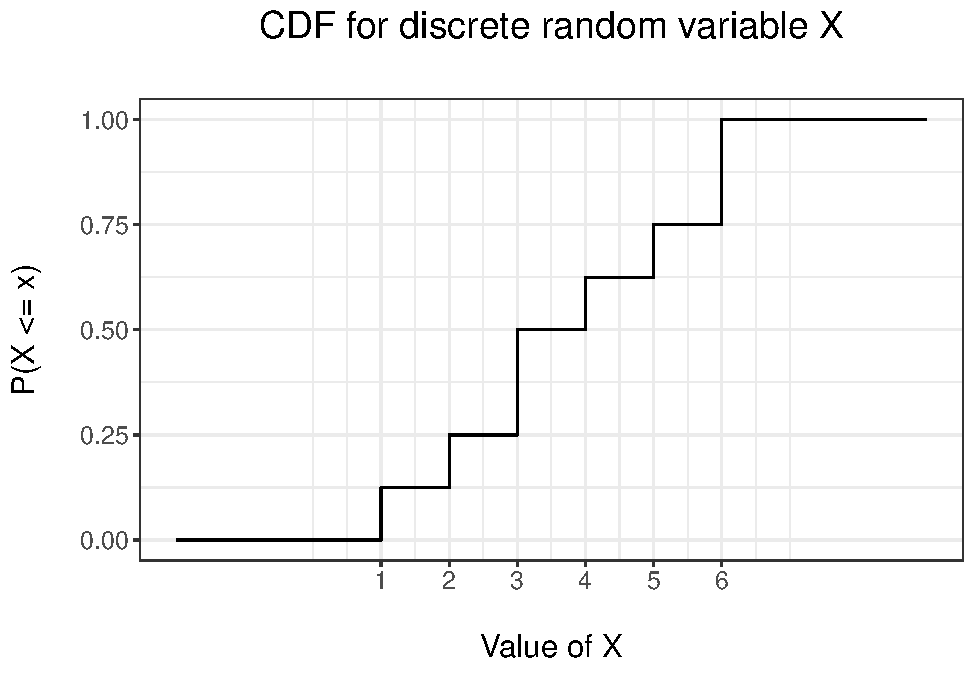
\includegraphics{SimBook_files/figure-latex/disc-cdf-1.pdf}
\caption{\label{fig:disc-cdf}CDF for the biased dice example}
\end{figure}

The plot highlights some properties of CDFs which can proved hold in general for any discrete CDF:

\begin{itemize}
\item
  it is a step function which is also non-decreasing;
\item
  on the left-hand-side it takes the value 0;
\item
  on the right-hand-side it takes the value 1.
\end{itemize}

\hypertarget{summaries}{%
\subsection{Summaries}\label{summaries}}

The pmf and the cdf fully characterize a discrete random variable \(X\). Often however we want to compress that information into a single number which still retains some aspect of the distribution of \(X\).

The \emph{expectation} or \emph{mean} of a random variable \(X\) denoted as \(E(X)\) is defined as
\[
E(X)=\sum_{x\in\mathbb{X}}xp(x)
\]
The expectation can be interpreted as the mean value of a large number of observations from the random variable \(X\). Consider again the example of the biased dice. The expectation is
\[
E(X)=1\cdot1/8 + 2\cdot1/8 + 3\cdot 2/8 + 4\cdot 1/8 + 5\cdot 1/8 + 6\cdot 2/8 = 3.75
\]
So if we were to throw the dice a large number of time, we would expect the average of the number shown to be 3.75.

The \emph{median} of the random variable \(X\) denoted as \(m(X)\) is defined as the value \(x\) such that \(P(X\leq x)\) is larger or equal to 0.5 and \(P(X\geq x)\) is larger or equal to 0.5. It is defined as the middle value of the distribution. For the dice example the median is the value 3: indeed \(P(X\leq 3 ) = P(X=1)+P(X=2)+P(X=3)=0.5 \geq 0.5\) and \(P(X\geq 3) = P(X=3) + P(X=4) + P(X=5) + P(X=6) = 0.75 \geq 0.5\).

The \emph{mode} of the random variable \(X\) is the value \(x\) such that \(p(x)\) is largest: it is the value of the random variable which is expected to happen most frequently. Notice that the mode may not be unique: in that case we say that the distribution of \(X\) is bimodal. The example of the biased dice as an instance of a bimodal distribution: the values 3 and 6 are the equally likely and they have the largest pmf.

The above three summaries are measures of \emph{centrality}: they describe the central tendency of \(X\). Next we consider measures of \emph{variability}: such measures will quantify the spread or the variation of the possible values of \(X\) around the mean.

The \emph{variance} of the discrete random variable \(X\) is the expectation of the squared difference between the random variable and its mean. Formally it is defined as
\[
V(X)=E((X-E(X))^2)=\sum_{x\in\mathbb{X}}(x-E(X))^2p(x)
\]
In general we will not compute variance by hand. The following R code computes the variance of the random variable associated to the biased dice.

\begin{Shaded}
\begin{Highlighting}[]
\NormalTok{x }\OtherTok{\textless{}{-}} \DecValTok{1}\SpecialCharTok{:}\DecValTok{6}  \CommentTok{\# outcomes of X}
\NormalTok{px }\OtherTok{\textless{}{-}} \FunctionTok{c}\NormalTok{(}\DecValTok{1}\SpecialCharTok{/}\DecValTok{8}\NormalTok{,}\DecValTok{1}\SpecialCharTok{/}\DecValTok{8}\NormalTok{,}\DecValTok{2}\SpecialCharTok{/}\DecValTok{8}\NormalTok{,}\DecValTok{1}\SpecialCharTok{/}\DecValTok{8}\NormalTok{,}\DecValTok{1}\SpecialCharTok{/}\DecValTok{8}\NormalTok{,}\DecValTok{2}\SpecialCharTok{/}\DecValTok{8}\NormalTok{)  }\CommentTok{\# pmf of X}
\NormalTok{Ex }\OtherTok{\textless{}{-}} \FunctionTok{sum}\NormalTok{(x}\SpecialCharTok{*}\NormalTok{px)  }\CommentTok{\# Expectation of X}
\NormalTok{Vx }\OtherTok{\textless{}{-}} \FunctionTok{sum}\NormalTok{((x}\SpecialCharTok{{-}}\NormalTok{Ex)}\SpecialCharTok{\^{}}\DecValTok{2}\SpecialCharTok{*}\NormalTok{px)  }\CommentTok{\# Variance of X}
\NormalTok{Vx}
\end{Highlighting}
\end{Shaded}

\begin{verbatim}
## [1] 2.9375
\end{verbatim}

The \emph{standard deviation} of the discrete random variable \(X\) is the square root of \(V(X)\).

\hypertarget{notable-discrete-variables}{%
\section{Notable Discrete Variables}\label{notable-discrete-variables}}

In the previous section we gave a generic definition of discrete random variables and discussed the conditions that a pmf must obey. We considered the example of a biased dice and constructed a pmf for that specific example.

There are situations that often happen in practice: for instance the case of experiments with binary outcomes. For such cases random variables with specific pmfs are given a name and their properties are well known and studied.

In this section we will consider three such distributions: Bernoulli, Binomial and Poisson.

\hypertarget{bernoulli-distribution}{%
\subsection{Bernoulli Distribution}\label{bernoulli-distribution}}

Consider an experiment or a real-world system where there can only be two outcomes:

\begin{itemize}
\item
  a toss of a coin: heads or tails;
\item
  the result of a COVID test: positive or negative;
\item
  the status of a machine: broken or working;
\end{itemize}

By default one outcome happens with some probability, that we denote as \(\theta\in [0,1]\) and the other with probability \(1-\theta\).

Such a situation is in general modeled using the so-called \emph{Bernoulli distribution} with parameter \(\theta\). One outcome is associated to the number 1 (usually referred to as sucess) and the other is associated to the number 0 (usually referred to as failure). So \(P(X=1)=p(1)=\theta\) and \(P(X=0)=p(0)=1-\theta\).

The above pmf can be more coincisely written as
\[
p(x)=\left\{
\begin{array}{ll}
\theta^x(1-\theta)^{1-x}, & x=0,1\\
0, & \mbox{otherwise}
\end{array}
\right.
\]
The mean and variance of the Bernoulli distribution can be easily computed as
\[
E(X)=0\cdot(1-\theta)+ 1\cdot\theta=\theta,
\]
and
\[
V(X)=(0-\theta)^2(1-\theta)+(1-\theta)^2\theta=\theta^2(1-\theta)+(1-\theta)^2\theta=\cdots = \theta(1-\theta)
\]

Figure \ref{fig:bernoulli} reports the pmf and the cdf of a Bernoulli random variable with parameter 0.3.

\begin{figure}
\centering
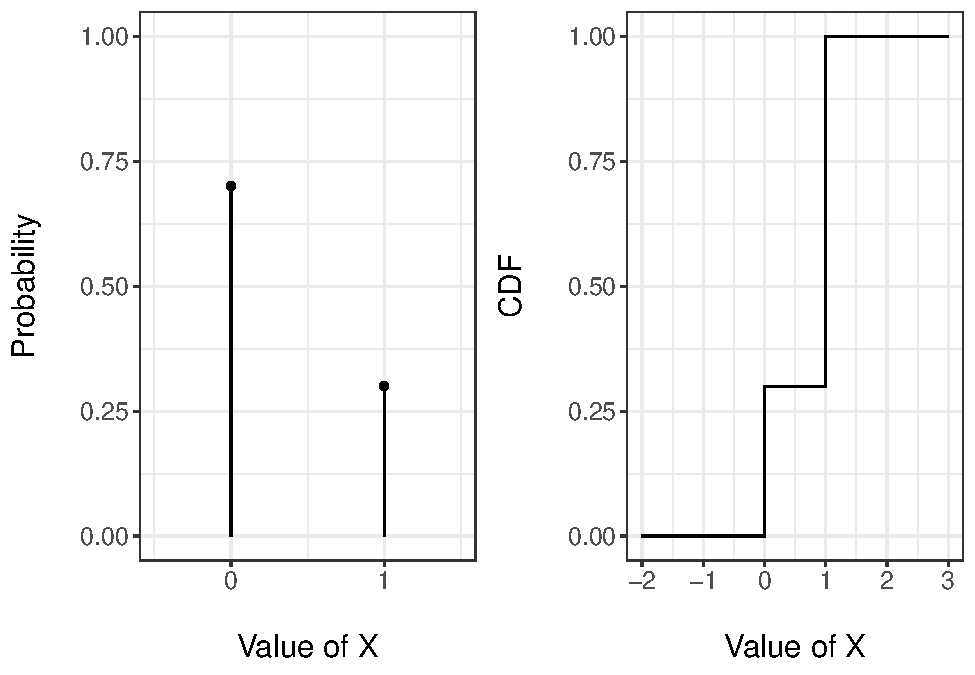
\includegraphics{SimBook_files/figure-latex/bernoulli-1.pdf}
\caption{\label{fig:bernoulli}PMF (left) and CDF (right) of a Bernoulli random variable with parameter 0.3}
\end{figure}

\hypertarget{binomial-distribution}{%
\subsection{Binomial Distribution}\label{binomial-distribution}}

The Bernoulli random variable is actually a very special case of the so-called \emph{Binomial} random variable. Consider experiments of the type discussed for Bernoullis: coin tosses, COVID tests etc. Now suppose that instead of having just one trial, each of these experiments are repeated multiple times. Consider the following assumptions:

\begin{itemize}
\item
  each experiment is repeated \(n\) times;
\item
  each time there is a probability of success \(\theta\);
\item
  the outcome of each experiment is independent of the others.
\end{itemize}

Let's think of tossing a coin \(n\) times. Then we would expect that the probability of showing heads is the same for all tosses and that the result of previous tosses does not affect others. So this situation appears to meet the above assumptions and can be modeled by what we call a Binomial random variable.

Formally, the random variable \(X\) is a Binomial random variable with parameters \(n\) and \(\theta\) if it denotes the number of successes of \(n\) independent Bernoulli random variables, all with parameter \(\theta\).

The pmf of a Binomial random variable with parameters \(n\) and \(\theta\) can be written as:
\[
p(x)=\left\{
\begin{array}{ll}
\binom{n}{x}\theta^{x}(1-\theta)^{n-x}, & x = 0,1,\dots,n\\
0, & \mbox{otherwise}
\end{array}
\right.
\]
Let's try and understand the formula by looking term by term.

\begin{itemize}
\item
  if \(X=x\) there are \(x\) successes and each success has probability \(\theta\) - so \(\theta^x\) counts the overall probability of successes
\item
  if \(X=x\) there are \(n-x\) failures and each failure has probability \(1-\theta\) - so \((1-\theta)^{n-x}\) counts the overall probability of failures
\item
  failures and successes can appear according to many orders. To see this, suppose that \(x=1\): there is only one success out of \(n\) trials. This could have been the first attempt, the second attempt or the \(n\)-th attempt. The term \(\binom{n}{x}\) counts all possible ways the outcome \(x\) could have happened.
\end{itemize}

The Bernoulli distribution can be seen as a special case of the Binomial where the parameter \(n\) is fixed to 1.

We will not show why this is the case but the expectation and the variance of the Binomial random variable with parameters \(n\) and \(\theta\) can be derived as
\[
E(X)=np, \hspace{2cm} V(X)=np(1-p)
\]
The formulae for the Bernoulli can be retrieved by setting \(n=1\).

Figure \ref{fig:binom} shows the pmf of two Binomial distributions both with parameter \(n=10\) and with \(\theta=0.3\) (left) and \(\theta=0.8\). For the case \(\theta=0.3\) we can see that it is more likely that there are a small number of successes, whilst for \(\theta=0.8\) a large number of successes is more likely.

\begin{figure}
\centering
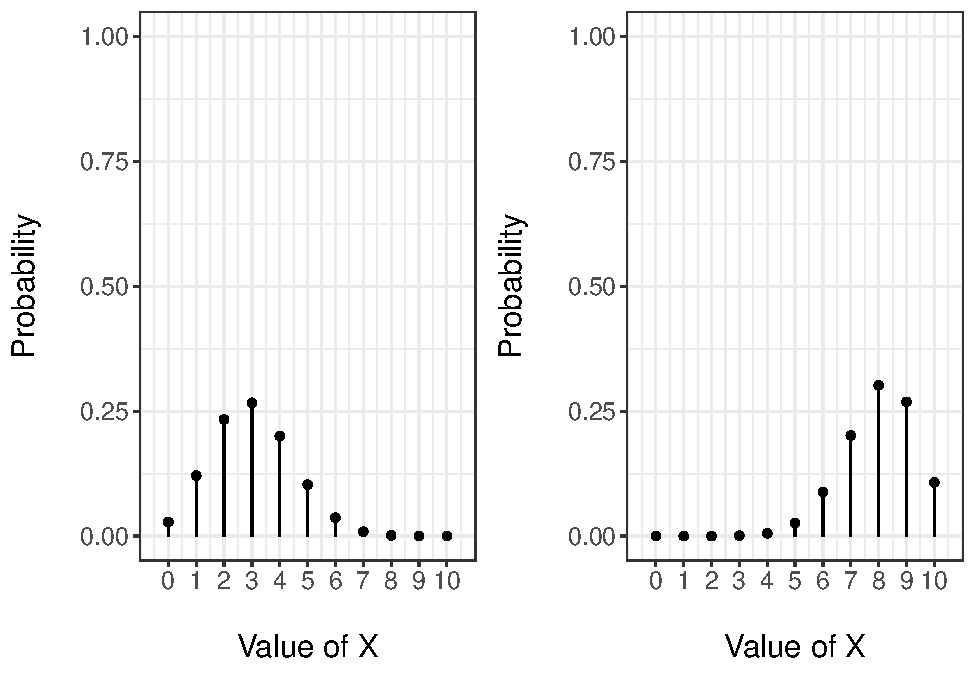
\includegraphics{SimBook_files/figure-latex/binom-1.pdf}
\caption{\label{fig:binom}PMF of a Binomial random variable with parameters n = 10 and theta = 0.3 (left) and theta = 0.8 (right)}
\end{figure}

R provides a straightforward implementation of the Binomial distribution through the functions \texttt{dbinom} for the pmf and \texttt{pbinom} for the cdf. They require three arguments:

\begin{itemize}
\item
  first argument is the value at which to compute the pmf or the cdf;
\item
  \texttt{size} is the parameter \(n\) of the Binomial;
\item
  \texttt{prob} is the parameter \(\theta\) of the Binomial.
\end{itemize}

So for instance

\begin{Shaded}
\begin{Highlighting}[]
\FunctionTok{dbinom}\NormalTok{(}\DecValTok{3}\NormalTok{, }\AttributeTok{size =} \DecValTok{10}\NormalTok{, }\AttributeTok{prob =} \FloatTok{0.5}\NormalTok{)}
\end{Highlighting}
\end{Shaded}

\begin{verbatim}
## [1] 0.1171875
\end{verbatim}

returns \(P(X=3)=p(3)\) for a Binomial random variable with parameter \(n=10\) and \(\theta = 0.5\).

Similarly,

\begin{Shaded}
\begin{Highlighting}[]
\FunctionTok{pbinom}\NormalTok{(}\DecValTok{8}\NormalTok{, }\AttributeTok{size =} \DecValTok{20}\NormalTok{, }\AttributeTok{prob =} \FloatTok{0.2}\NormalTok{)}
\end{Highlighting}
\end{Shaded}

\begin{verbatim}
## [1] 0.9900182
\end{verbatim}

returns \(P(X\leq 8) = F(8)\) for a Binomial random variable with parameter \(n=20\) and \(\theta = 0.2\).

\hypertarget{poisson-distribution}{%
\subsection{Poisson Distribution}\label{poisson-distribution}}

The last class of discrete random variables we discuss is the so-called \emph{Poisson} distribution. Whilst for Bernoulli and Binomial we had an interpretation of why the pmf took its specific form by associating it to independent binary experiments each with an equal probability of success, for the Poisson there is no such an interpretation.

A discrete random variable \(X\) has a Poisson distribution with parameter \(\lambda\) if its pmf is
\[
p(x)=\left\{
\begin{array}{ll}
\frac{e^{-\lambda}\lambda^x}{x!}, & x = 0,1,2,3,\dots\\
0, & \mbox{otherwise}
\end{array}
\right.
\]
where \(\lambda > 0\).

So the sample space of a Poisson random variable is the set of all non-negative integers.

One important characteristic of the Poisson distribution is that its mean and variance are equal to the parameter \(\lambda\), that is
\[
E(X)= V(X) = \lambda.
\]

Figure @ref\{fig:poisson\} gives an illustration of the form of the pmf of the Poisson distribution for two parameter choices: \(\lambda=1\) (left) and \(\lambda = 4\) (right). The x-axis is shown until \(x=10\) but recall that the Poisson is defined over all non-negative integers. For the case \(\lambda=1\) we can see that the outcomes 0 and 1 have the largest probability - recall that \(E(X)=0\). For the case \(\lambda = 4\) the outcomes \(x = 2,3,4,5\) have the largest probability.

\begin{figure}
\centering
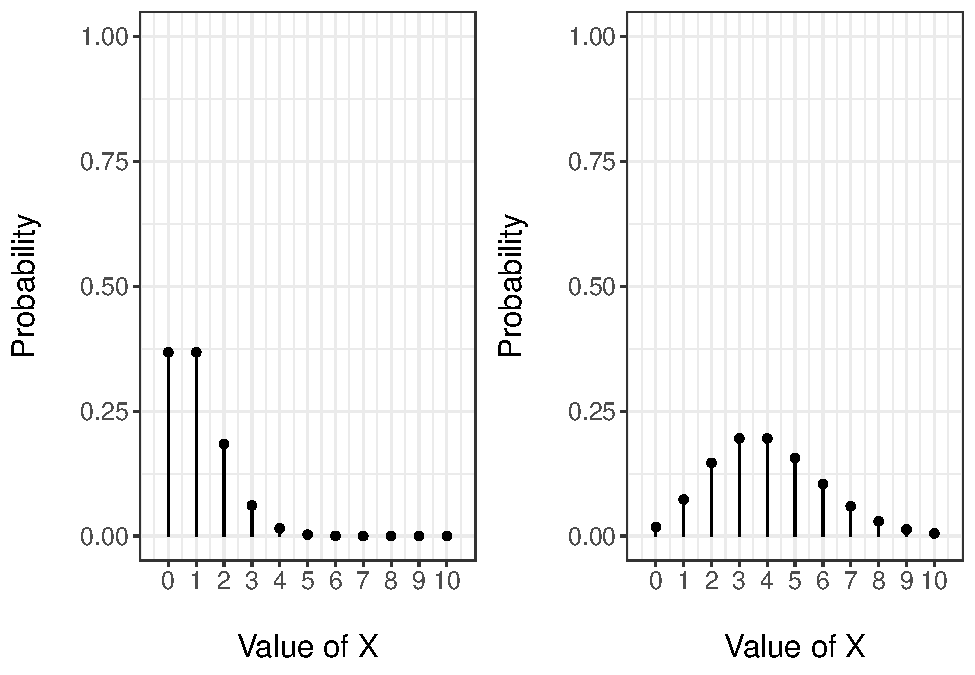
\includegraphics{SimBook_files/figure-latex/poisson-1.pdf}
\caption{\label{fig:poisson}PMF of a Poisson random variable with parameter 1 (left) and 4 (right)}
\end{figure}

R provides a straightforward implementation of the Poisson distribution through the functions \texttt{dpois} for the pmf and \texttt{ppois} for the cdf. They require three arguments:

\begin{itemize}
\item
  first argument is the value at which to compute the pmf or the cdf;
\item
  \texttt{lambda} is the parameter \(\lambda\) of the Poisson;
\end{itemize}

So for instance

\begin{Shaded}
\begin{Highlighting}[]
\FunctionTok{dpois}\NormalTok{(}\DecValTok{3}\NormalTok{, }\AttributeTok{lambda =} \DecValTok{1}\NormalTok{)}
\end{Highlighting}
\end{Shaded}

\begin{verbatim}
## [1] 0.06131324
\end{verbatim}

returns \(P(X=3)=p(3)\) for a Poisson random variable with parameter \(\lambda = 1\).

Similarly,

\begin{Shaded}
\begin{Highlighting}[]
\FunctionTok{ppois}\NormalTok{(}\DecValTok{8}\NormalTok{, }\AttributeTok{lambda =} \DecValTok{4}\NormalTok{)}
\end{Highlighting}
\end{Shaded}

\begin{verbatim}
## [1] 0.9786366
\end{verbatim}

returns \(P(X\leq 8) = F(8)\) for a Poisson random variable with parameter \(\lambda = 4\).

\hypertarget{some-examples}{%
\subsection{Some Examples}\label{some-examples}}

We next consider two examples to see in practice the use of the Binomial and Poisson distributions.

\hypertarget{probability-of-marriage}{%
\subsubsection{Probability of Marriage}\label{probability-of-marriage}}

A recent survey indicated that 82\% of single women aged 25 years old will be married in their lifetime. Compute

\begin{itemize}
\item
  the probability of at most 3 women will be married in a sample of 20;
\item
  the probability of at least 90 women will be married in sample of 100;
\item
  the probability of two or three women in a sample of 20 will never be married.
\end{itemize}

The above situation can be modeled by a Binomial random variable where the parameter \(n\) depends on the question and \(\theta = 0.82\).

The first question requires us to compute \(P(X\leq 3)= F(3)\) where \(X\) is Binomial with parameters \(n=20\) and \(\theta =0.82\). Using R

\begin{Shaded}
\begin{Highlighting}[]
\FunctionTok{pbinom}\NormalTok{(}\DecValTok{3}\NormalTok{, }\AttributeTok{size =} \DecValTok{10}\NormalTok{, }\AttributeTok{prob =} \FloatTok{0.82}\NormalTok{)}
\end{Highlighting}
\end{Shaded}

\begin{verbatim}
## [1] 0.0004400767
\end{verbatim}

The second question requires us to compute \(P(X\geq 90)\) where \(X\) is a Binomial random variable with parameters \(n=100\) and \(\theta = 0.82\). Notice that
\[
P(X\geq 90) = 1 - P(X< 90) = 1 - P(X\leq 89) = 1 - F(89).
\]
Using R

\begin{Shaded}
\begin{Highlighting}[]
\DecValTok{1} \SpecialCharTok{{-}} \FunctionTok{pbinom}\NormalTok{(}\DecValTok{89}\NormalTok{, }\AttributeTok{size =} \DecValTok{100}\NormalTok{,  }\AttributeTok{prob =} \FloatTok{0.82}\NormalTok{)}
\end{Highlighting}
\end{Shaded}

\begin{verbatim}
## [1] 0.02003866
\end{verbatim}

For the third question, notice that saying two women out of 20 will never be married is equal to 18 out of 20 will be married. Therefore we need to compute \(P(X=17) + P(X=18)= p(17) + p(18)\) where \(X\) is a Binomial random variable with parameters \(n=20\) and \(\theta = 0.82\). Using R

\begin{Shaded}
\begin{Highlighting}[]
\FunctionTok{sum}\NormalTok{(}\FunctionTok{dbinom}\NormalTok{(}\DecValTok{17}\SpecialCharTok{:}\DecValTok{18}\NormalTok{, }\AttributeTok{size =} \DecValTok{20}\NormalTok{, }\AttributeTok{prob =} \FloatTok{0.82}\NormalTok{))}
\end{Highlighting}
\end{Shaded}

\begin{verbatim}
## [1] 0.4007631
\end{verbatim}

\hypertarget{the-bad-stuntman}{%
\subsubsection{The Bad Stuntman}\label{the-bad-stuntman}}

A stuntman injures himself an average of three times a year. Use the Poisson probability formula to calculate the probability that he will be injured:

\begin{itemize}
\item
  4 times a year
\item
  Less than twice this year.
\item
  More than three times this year.
\end{itemize}

The above situation can be modeled as a Poisson distribution \(X\) with parameter \(\lambda = 3\).

The first question requires us to compute \(P(X=4)\) which using R can be computed as

\begin{Shaded}
\begin{Highlighting}[]
\FunctionTok{dpois}\NormalTok{(}\DecValTok{4}\NormalTok{, }\AttributeTok{lambda =}\DecValTok{3}\NormalTok{)}
\end{Highlighting}
\end{Shaded}

\begin{verbatim}
## [1] 0.1680314
\end{verbatim}

The second question requires us to compute \(P(X<2) = P(X=0)+P(X=1)= F(1)\) which using R can be computed as

\begin{Shaded}
\begin{Highlighting}[]
\FunctionTok{ppois}\NormalTok{(}\DecValTok{1}\NormalTok{,}\AttributeTok{lambda=}\DecValTok{3}\NormalTok{)}
\end{Highlighting}
\end{Shaded}

\begin{verbatim}
## [1] 0.1991483
\end{verbatim}

The third question requires us to compute \(P(X>3) = 1 - P(X\leq 2) = 1 - F(2)\) which using R can be computed as

\begin{Shaded}
\begin{Highlighting}[]
\DecValTok{1} \SpecialCharTok{{-}} \FunctionTok{ppois}\NormalTok{(}\DecValTok{2}\NormalTok{, }\AttributeTok{lambda =} \DecValTok{3}\NormalTok{)}
\end{Highlighting}
\end{Shaded}

\begin{verbatim}
## [1] 0.5768099
\end{verbatim}

\hypertarget{continuous-random-variables}{%
\section{Continuous Random Variables}\label{continuous-random-variables}}

Our attention now turns to continuous random variables. These are in general more technical and less intuitive than discrete ones. You should not worry about all the technical details, since these are in general not important, and focus on the interpretation.

A continuous random variable \(X\) is a random variable whose sample space \(\mathbb{X}\) is an interval or a collection of intervals. In general \(\mathbb{X}\) may coincide with the set of real numbers \(\mathbb{R}\) or some subset of it. Examples of continuous random variables:

\begin{itemize}
\item
  the pressure of a tire of a car: it can be any positive real number;
\item
  the current temperature in the city of Madrid: it can be any real number;
\item
  the height of the students of Simulation and Modeling to understand change: it can be any real number.
\end{itemize}

Whilst for discrete random variables we considered summations over the elements of \(\mathbb{X}\), i.e.~\(\sum_{x\in\mathbb{X}}\), for continuous random variables we need to consider integrals over appropriate intervals.

You should be more or less familiar with these from previous studies of calculus. But let's give an example. Consider the function \(f(x)=x^2\) computing the squared of a number \(x\). Suppose we are interested in this function between the values -1 and 1, which is plotted by the red line in Figure \ref{fig:x-sq}. Consider the so-called integral \(\int_{-1}^{1}x^2dx\): this coincides with the area delimited by the function and the x-axis. In Figure \ref{fig:x-sq} the blue area is therefore equal to \(\int_{-1}^{1}x^2dx\).

\begin{figure}

{\centering 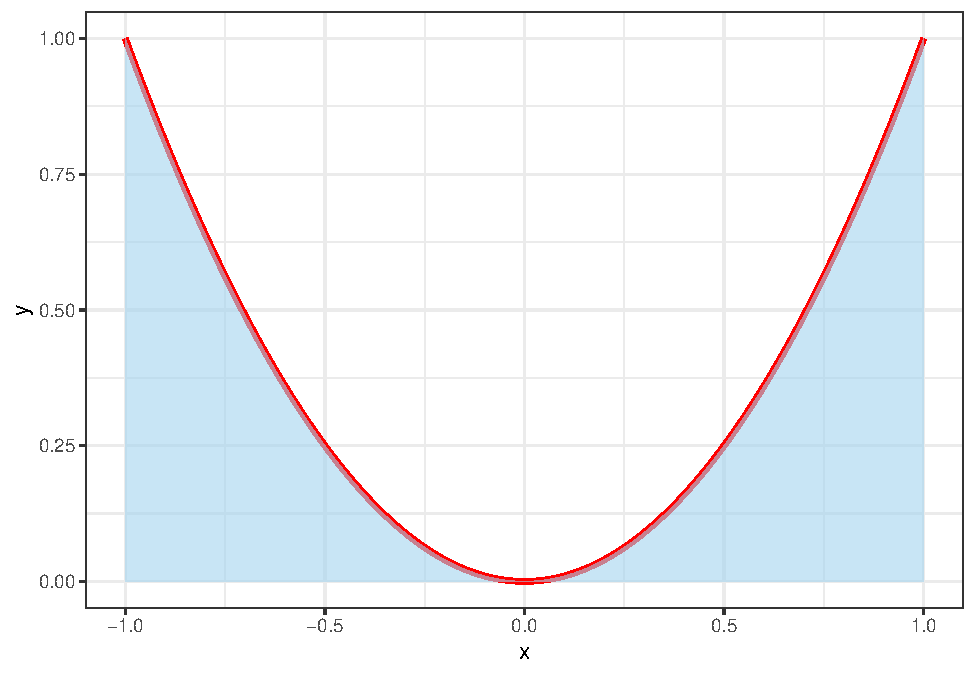
\includegraphics[width=0.5\linewidth]{SimBook_files/figure-latex/x-sq-1} 

}

\caption{Plot of the squared function and the area under its curve}\label{fig:x-sq}
\end{figure}

We will not be interested in computing integrals ourselves, so if you do not know/remember how to do it, there is no problem!

\hypertarget{probability-density-function}{%
\subsection{Probability Density Function}\label{probability-density-function}}

Discrete random variable are easy to work with in the sense that there exists a function, that we called probability mass function, such that \(p(x)=P(X=x)\), that is the value of that function in the point \(x\) is exactly the probability that \(X=x\).

Therefore we may wonder if this is true for a continuous random variable too. Sadly, the answer is no and probabilities for continuous random variables are defined in a slightly more involved way.

Let \(X\) be a continuous random variable with sample space \(\mathbb{X}\). The probability that \(X\) takes values in the interval \([a,b]\) is given by
\[
P(a\leq X \leq b) = \int_{a}^bf(x)dx
\]
where \(f(x)\) is called the \emph{probability density function} (pdf in short). Pdfs, just like pmfs must obey two conditions:

\begin{itemize}
\item
  \(f(x)\geq 0\) for all \(x\in\mathbb{X}\);
\item
  \(\int_{x\in\mathbb{X}}f(x)dx=1\).
\end{itemize}

So in the discrete case the pmf is defined exactly as the probability. In the continuous case the pdf is the function such that its integral is the probability that random variable takes values in a specific interval.

As a consequence of this definition notice that for any specific value \(x_0\in\mathbb{X}\), \(P(X=x_0)=0\) since
\[
\int_{x_0}^{x_0}f(x)dx = 0.
\]

Let's consider an example. The waiting time of customers of a donuts shop is believed to be random and to follow a random variable whose pdf is
\[
f(x) = \left\{
\begin{array}{ll}
\frac{1}{4}e^{-x/4}, & x\geq 0\\
0, & \mbox{otherwise}
\end{array}
\right.
\]

The pdf is drawn in Figure \ref{fig:exp} by the red line. One can see that \(f(x)\geq 0\) for all \(x\geq 0\) and one could also compute that it integrates to one.

Therefore the probability that the waiting time is between any two values \((a,b)\) can be computed as
\[
\int_a^b\frac{1}{4}e^{-x/4}dx.
\]
In particular if we were interested in the probability that the waiting time is between two and five minutes, corresponding to the shaded area in Figure \ref{fig:exp}, we could compute it as
\[
P(2<X<5)=\int_2^5f(x)dx=\int_{2}^5\frac{1}{4}e^{-x/4}dx= 0.32
\]

\begin{figure}

{\centering 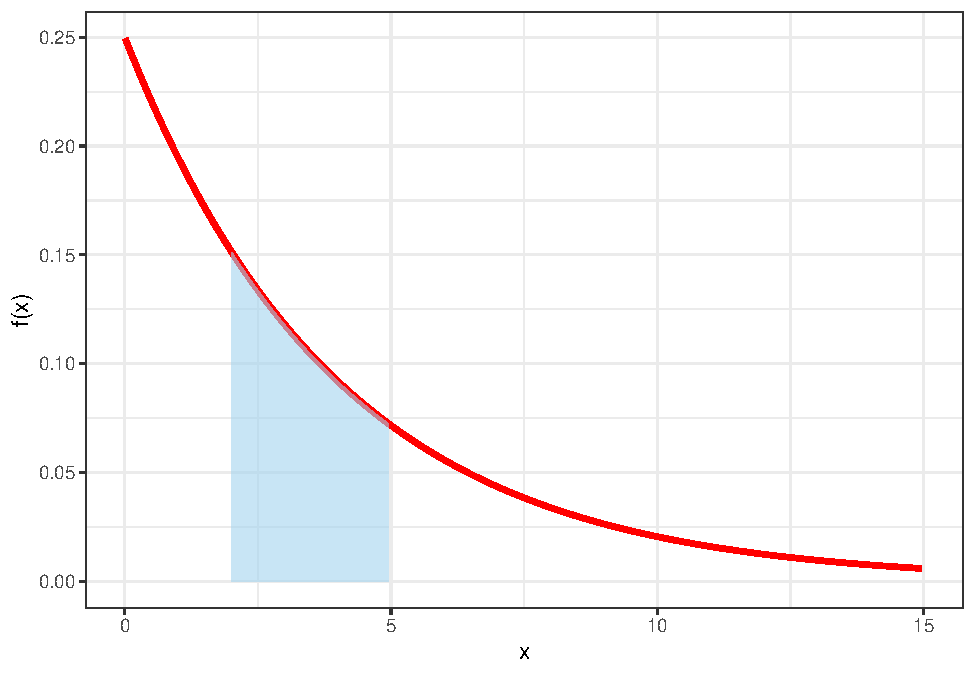
\includegraphics[width=0.5\linewidth]{SimBook_files/figure-latex/exp-1} 

}

\caption{Probability density function for the waiting time in the donut shop example}\label{fig:exp}
\end{figure}

Notice that since \(P(X=x_0)=0\) for any \(x_0\in\mathbb{X}\), we also have that
\[
P(a\leq X \leq b)=P(a < X \leq b) = P(a\leq X < b) = P(a<X<b).
\]

\hypertarget{cumulative-distribution-function-1}{%
\subsection{Cumulative Distribution Function}\label{cumulative-distribution-function-1}}

For a continuous random variable \(X\) the cumulative distribution function (cdf) is equally defined as
\[
F(x) = P(X \leq x),
\]
where now
\[
P(X \leq x) = P(X < x) = \int_{-\infty}^xf(t)dt.
\]
so the summation is substituted by an integral.

Let's consider again the donut shop example as an illustration. The cdf is defined as
\[
F(x)=\int_{-\infty}^xf(t)dt = \int_{-\infty}^x\frac{1}{4}e^{-x/4}.
\]
This integral can be solved and \(F(x)\) can be calculated as
\[
F(x)= 1- e^{-x/4},
\]
which is plotted in Figure \ref{fig:expcdf}.

\begin{figure}

{\centering 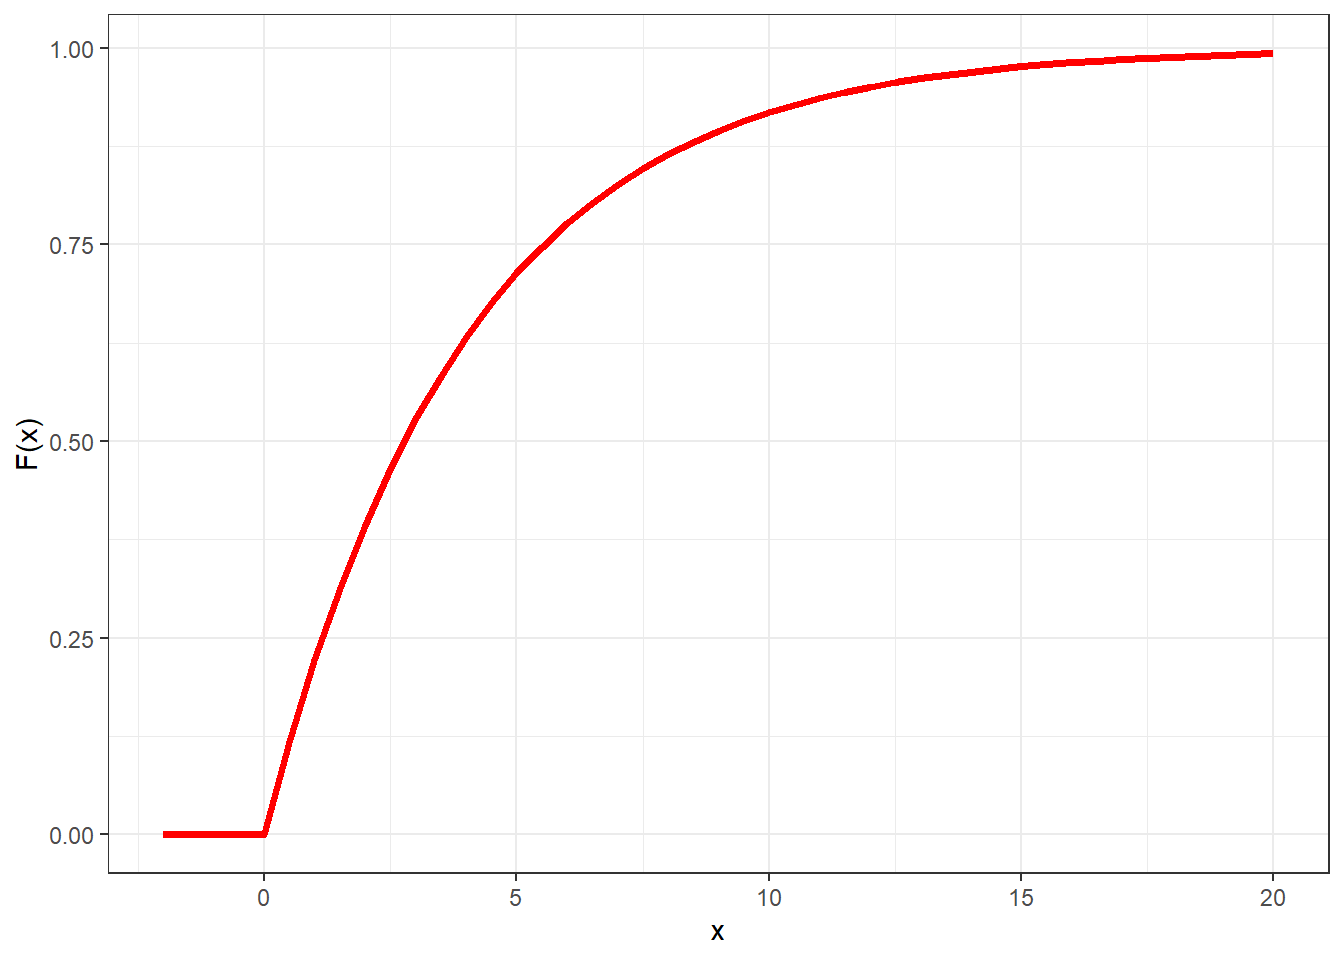
\includegraphics[width=0.5\linewidth]{SimBook_files/figure-latex/expcdf-1} 

}

\caption{Cumulative distribution function for the waiting time at the donut shop}\label{fig:expcdf}
\end{figure}

We can notice that the cdf has similar properties as in the discrete case: it is non-decreasing, on the left-hand side is zero and on the right-hand side tends to zero.

\hypertarget{summaries-1}{%
\subsection{Summaries}\label{summaries-1}}

Just as for discrete random variables, we may want to summarize some features of a continuous random variable into a unique number. The same set of summaries exists for continuous random variables, which are almost exactly defined as in the discrete case (integrals are used instead of summations).

\begin{itemize}
\item
  \emph{mean}: the mean of a continuous random variable \(X\) is defined as
  \[
   E(X) = \int_{-\infty}^{+\infty}xf(x)dx
   \]
\item
  \emph{median}: the median of a continuous random variable \(X\) is defined as the value \(x\) such that \(P(X\leq x) = 0.5\) or equally \(F(x)=0.5\).
\item
  \emph{mode}: the mode of a continuous random variable \(X\) is defined the value \(x\) such that \(f(x)\) is largest.
\item
  \emph{variance}: the variance of a continuous random variable \(X\) is defined as
  \[
   V(X)=\int_{-\infty}^{+\infty}(x-E(X))^2f(x)dx
   \]
\item
  \emph{standard deviation}: the standard deviation of a continuous random variable \(X\) is defined as \(\sqrt{V(X)}\).
\end{itemize}

\hypertarget{notable-continuous-distribution}{%
\section{Notable Continuous Distribution}\label{notable-continuous-distribution}}

As in the discrete case, there are some types of continuous random variables that are used frequently and therefore are given a name and their proprieties are well-studied.

\hypertarget{uniform-distribution}{%
\subsection{Uniform Distribution}\label{uniform-distribution}}

The first, and simplest, continuous random variable we study is the so-called (continuous) \emph{uniform} distribution. We say that a random variable \(X\) is uniformly distributed on the interval \([a,b]\) if its pdf is
\[
f(x)=\left\{ 
\begin{array}{ll}
\frac{1}{b-a}, & a\leq x \leq b\\
0, & \mbox{otherwise} 
\end{array}
\right.
\]
This is plotted in Figure \ref{fig:unipdf} for choices of parameters \(a=2\) and \(b=6\)

\begin{figure}

{\centering 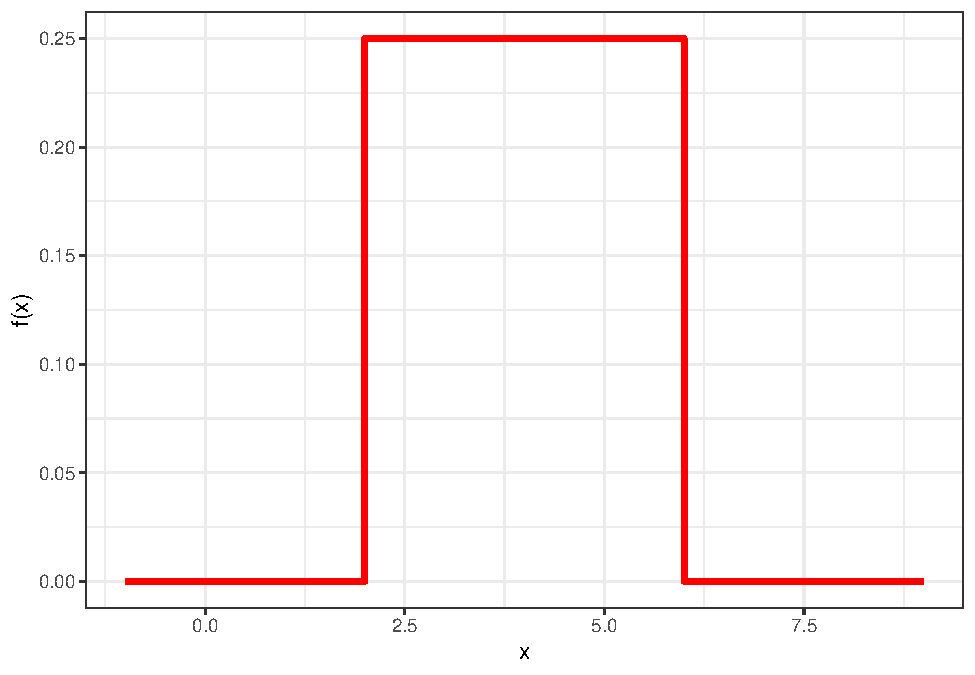
\includegraphics[width=0.5\linewidth]{SimBook_files/figure-latex/unipdf-1} 

}

\caption{Probability density function for a uniform random variable with parameters a = 2 and b = 6}\label{fig:unipdf}
\end{figure}

By looking at the pdf we see that it is a flat, constant line between the values \(a\) and \(b\). This implies that the probability that \(X\) takes values between two values \(x_0\) and \(x_1\) only dependens on the length of the interval \((x_0,x_1)\).

Its cdf can be derived as
\[
F(x)=\left\{
\begin{array}{ll}
0, & x<a\\
\frac{x-a}{b-a}, & a\leq x \leq b\\
1, & x>b
\end{array}
\right.
\]
and this is plotted in Figure \ref{fig:unicdf}.

\begin{figure}

{\centering 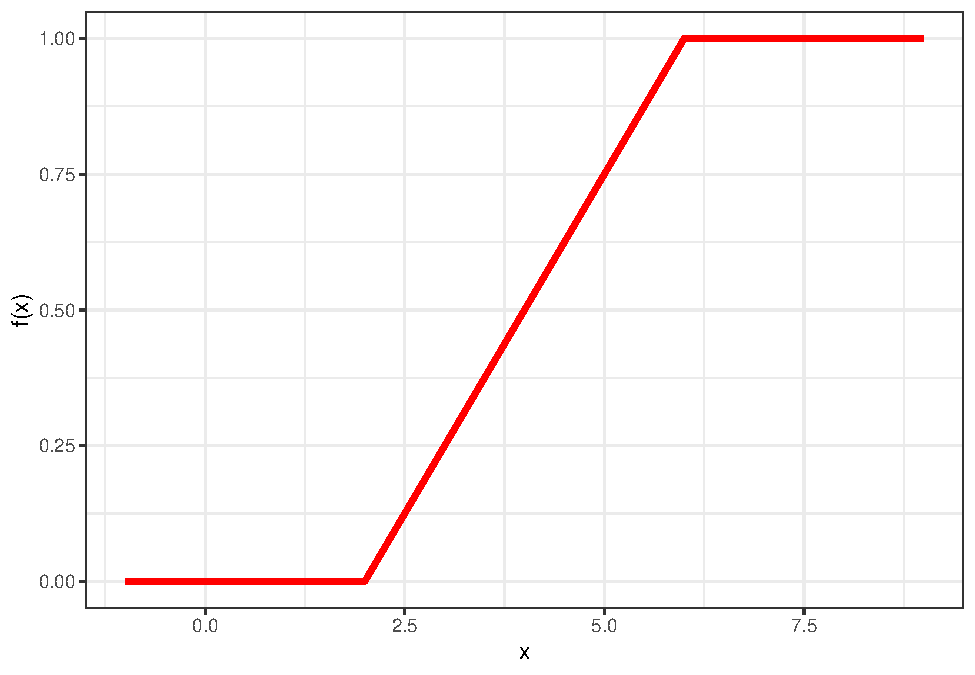
\includegraphics[width=0.5\linewidth]{SimBook_files/figure-latex/unicdf-1} 

}

\caption{Cumulative distribution function for a uniform random variable with parameters a = 2 and b = 6}\label{fig:unicdf}
\end{figure}

The mean and variance of a uniform can be derived as
\[
E(X)=\frac{a+b}{2}, \hspace{1cm} V(X)=\frac{(b-a)^2}{12}.
\]
So the mean is equal to the middle point of the interval \((a,b)\).

The uniform distribution will be fundamental in simulation. We will see that the starting point to simulate random numbers from any distribution will require the simulation of random numbers uniformly distributed between 0 and 1.

R provides an implementation of the uniform random variable with the functions \texttt{dunif} and \texttt{punif} whose details are as follows:

\begin{itemize}
\item
  the first argument is the value at which to compute the function;
\item
  the second argument, \texttt{min}, is the parameter \(a\), by default equal to zero;
\item
  the third argument, \texttt{max}, is the parameter \(b\), by default equal to one.
\end{itemize}

So for instance

\begin{Shaded}
\begin{Highlighting}[]
\FunctionTok{dunif}\NormalTok{(}\DecValTok{5}\NormalTok{, }\AttributeTok{min =} \DecValTok{2}\NormalTok{, }\AttributeTok{max =} \DecValTok{6}\NormalTok{)}
\end{Highlighting}
\end{Shaded}

\begin{verbatim}
## [1] 0.25
\end{verbatim}

computes the pdf at the point 5 of a uniform random variable with parameters \(a=2\) and \(b=6\).

Conversely,

\begin{Shaded}
\begin{Highlighting}[]
\FunctionTok{punif}\NormalTok{(}\FloatTok{0.5}\NormalTok{)}
\end{Highlighting}
\end{Shaded}

\begin{verbatim}
## [1] 0.5
\end{verbatim}

computes the cdf at the point 0.5 of a uniform random variable with parameters \(a=0\) and \(b=1\).

\hypertarget{exponential-distribution}{%
\subsection{Exponential Distribution}\label{exponential-distribution}}

The second class of continuous random variables we will study are the so-called \emph{exponential} random variables. We have actually already seen such a random variable in the donut shop example. More generally, we say that a continuous random variable \(X\) is exponential with parameter \(\lambda>0\) if its pdf is
\[
f(x) = \left\{
\begin{array}{ll}
\lambda e^{-\lambda x}, & x\geq 0\\
0, & \mbox{otherwise}
\end{array}
\right.
\]

Figure \ref{fig:exppdf1} reports the pdf of exponential random variables for various choices of the parameter \(\lambda\).

\begin{figure}

{\centering 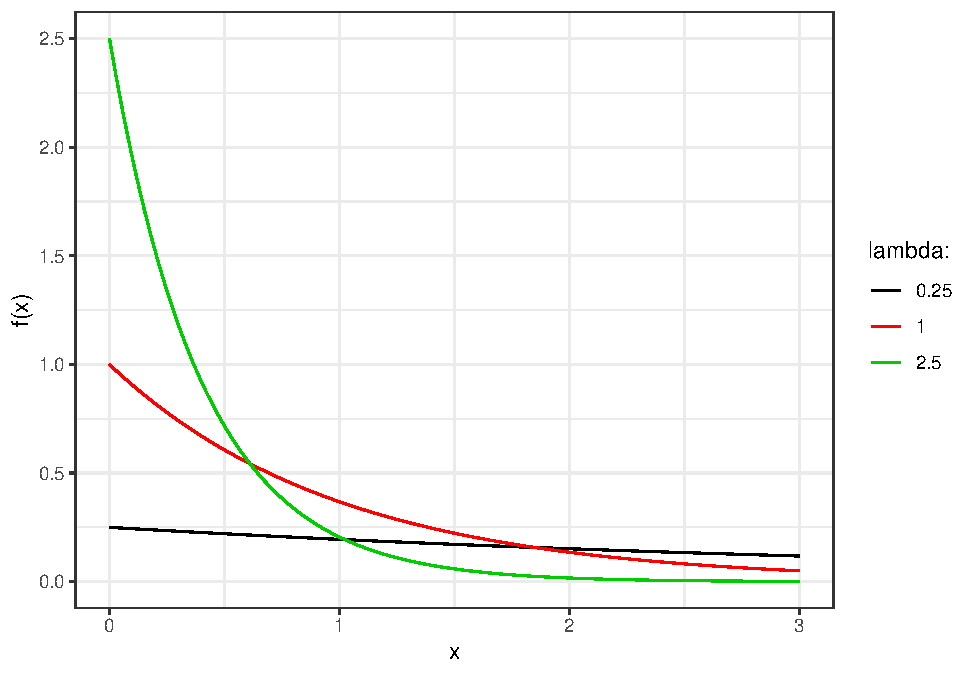
\includegraphics[width=0.5\linewidth]{SimBook_files/figure-latex/exppdf1-1} 

}

\caption{Probability density function for exponential random variables}\label{fig:exppdf1}
\end{figure}

Exponential random variables are very often used in dynamic simulations since they are very often used to model interarrival times in process: for instance the time between arrivals of customers at the donut shop.

Its cdf can be derived as
\[
F(x)=\left\{
\begin{array}{ll}
0, & x <0\\
1-e^{-\lambda x}, & x\geq 0
\end{array}
\right.
\]
and is reported in Figure \ref{fig:expcdf1} for the same choices of parameters.

\begin{figure}

{\centering 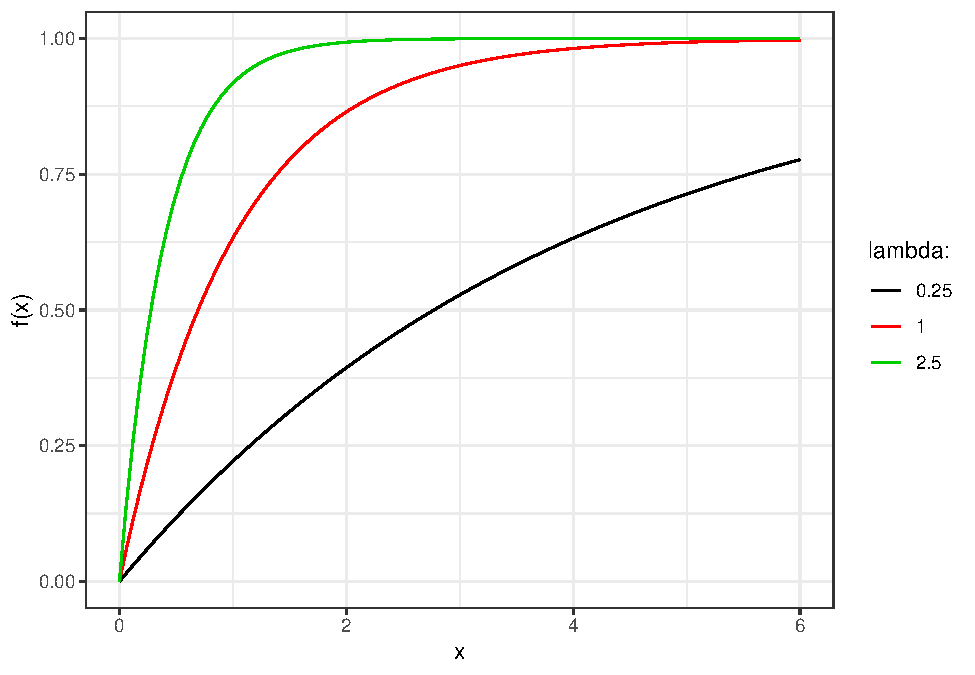
\includegraphics[width=0.5\linewidth]{SimBook_files/figure-latex/expcdf1-1} 

}

\caption{Cumulative distribution function for exponential random variables}\label{fig:expcdf1}
\end{figure}

The mean and the variance of exponential random variables can be computed as

\[
E(X)=\frac{1}{\lambda}, \hspace{1cm} V(X)=\frac{1}{\lambda^2}
\]

R provides an implementation of the uniform random variable with the functions \texttt{dexp} and \texttt{pexp} whose details are as follows:

\begin{itemize}
\item
  the first argument is the value at which to compute the function;
\item
  the second argument, \texttt{rate}, is the parameter \(\lambda\), by default equal to one;
\end{itemize}

So for instance

\begin{Shaded}
\begin{Highlighting}[]
\FunctionTok{dexp}\NormalTok{(}\DecValTok{2}\NormalTok{, }\AttributeTok{rate =} \DecValTok{3}\NormalTok{)}
\end{Highlighting}
\end{Shaded}

\begin{verbatim}
## [1] 0.007436257
\end{verbatim}

computes the pdf at the point 2 of an exponential random variable with parameter \(\lambda =3\).

Conversely

\begin{Shaded}
\begin{Highlighting}[]
\FunctionTok{pexp}\NormalTok{(}\DecValTok{4}\NormalTok{)}
\end{Highlighting}
\end{Shaded}

\begin{verbatim}
## [1] 0.9816844
\end{verbatim}

computes the cdf at the point 4 of an exponential random variable with parameter \(\lambda =1\).

\hypertarget{normal-distribution}{%
\subsection{Normal Distribution}\label{normal-distribution}}

The last class of continuous random variables we consider is the so-called \emph{Normal} or \emph{Gaussian} random variable. They are the most used and well-known random variable in statistics and we will see why this is the case.

A continuous random variable \(X\) is said to have a Normal distribution with mean \(\mu\) and variance \(\sigma^2\) if its pdf is
\[
f(x) = \frac{1}{\sqrt{2\pi\sigma^2}}\exp\left(-\frac{1}{2}\frac{(x-\mu)^2}{\sigma^2}\right).
\]
Recall that
\[
E(X)=\mu, \hspace{1cm} V(X)=\sigma^2,
\]
and so the parameters have a straightforward interpretation in terms of mean and variance.

Figure \ref{fig:norm} shows the form of the pdf of the Normal distribution for various choices of the parameters. On the left we have Normal pdfs for \(\sigma^2=1\) and various choices of \(\mu\): we can see that \(\mu\) shifts the plot on the x-axis. On the right we have Normal pdfs for \(\mu=1\) and various choices of \(\sigma^2\): we can see that all distributions are centered around the same value while they have a different spread/variability.

\begin{figure}

{\centering 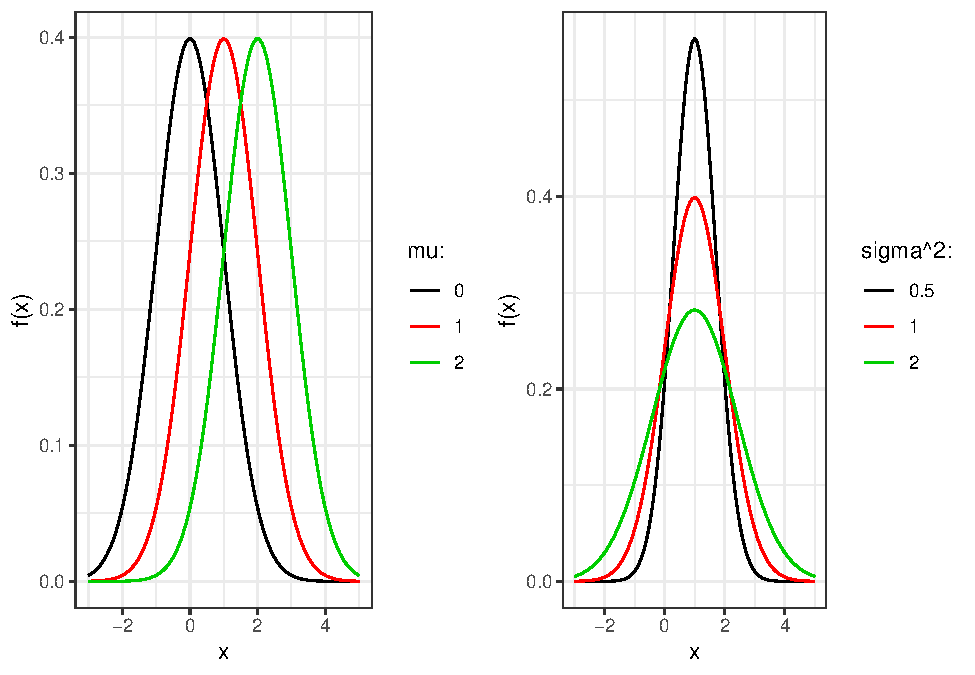
\includegraphics[width=0.5\linewidth]{SimBook_files/figure-latex/norm-1} 

}

\caption{Probability density function for normal random variables}\label{fig:norm}
\end{figure}

The form of the Normal pdf is the well-known so-called bell-shaped function. We can notice some properties:

\begin{itemize}
\item
  it is symmetric around the mean: the function on the left-hand side and on the right-hand side of the mean is mirrored. This implies that the median is equal to the mean ;
\item
  the maximum value of the pdf occurs at the mean. This implies that the mode is equal to the mean (and therefore also the median).
\end{itemize}

The cdf of the Normal random variable with parameters \(\mu\) and \(\sigma^2\) is
\[
F(x) = P(X\leq x)=\int_{-\infty}^{+\infty}\frac{1}{\sqrt{2\pi\sigma^2}}\exp\left(-\frac{1}{2}\frac{(x-\mu)^2}{\sigma^2}\right)dx
\]

The cdf of the Normal for various choices of parameters is reported in Figure \ref{fig:pnorm}.

\begin{figure}

{\centering 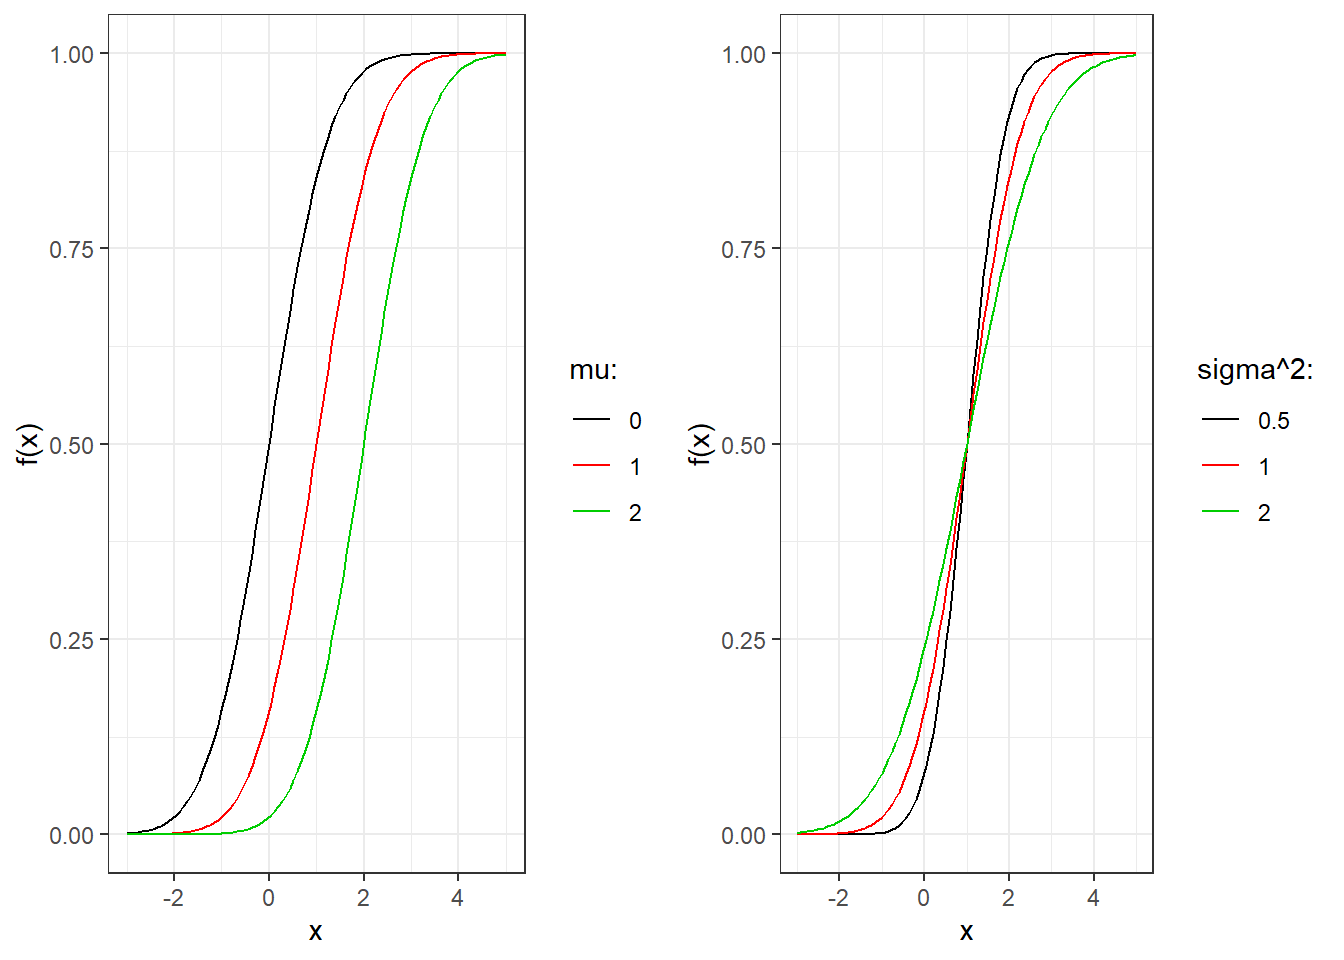
\includegraphics[width=0.5\linewidth]{SimBook_files/figure-latex/pnorm-1} 

}

\caption{Cumulative distribution function for normal random variables}\label{fig:pnorm}
\end{figure}

Unfortunately it is not possible to solve such an integral (as for example for the Uniform and the Exponential), and in general it is approximated using some numerical techniques. This is surprising considering that the Normal distribution is so widely used!!!

However, notice that we would need to compute such an approximation for every possible value of \((\mu,\sigma^2)\), depending on the distribution we want to use. This is unfeasible to do in practice.

There is a trick here, that you must have used multiple times already. We can transform a Normal \(X\) with parameters \(\mu\) and \(\sigma^2\) to the so-called \emph{standard Normal} random variable \(Z\), and viceversa, using the relationship:
\begin{equation}
 \label{eq:standard}
Z = \frac{X-\mu}{\sigma}, \hspace{1cm} X= \mu + \sigma Z.
\end{equation}
It can be shown that \(Z\) is a Normal random variable with parameter \(\mu=0\) and \(\sigma^2=1\).

The values of the cdf of the standard Normal random variable then need to be computed only once since \(\mu\) and \(\sigma^2\) are fixed. You have seen these numbers many many times in what are usually called the tables of the Normal distribution.

As a matter of fact you have also computed many times the cdf of a generic Normal random variable. First you computed \(Z\) using equation \eqref{eq:standard} and then looked at the Normal tables to derive that number.

Let's give some details about the standard Normal. Its pdf is
\[
\phi(z)=\frac{1}{\sqrt{2\pi}}\exp\left(-z^2/2\right).
\]
It can be seen that it is the same as the one of the Normal by setting \(\mu=0\) and \(\sigma^2=1\). Such a function is so important that it is given its own symbol \(\phi\).

The cdf is
\[
\Phi(z)=\int_{-\infty}^z\frac{1}{\sqrt{2\pi}}\exp\left(-x^2/2\right)dx
\]
Again this cannot be computed exactly, there is no closed-form expression. This is why you had to look at the tables instead of using a simple formula. The cdf of the standard Normal is also so important that it is given its own symbol \(\phi\).

Instead of using the tables, we can use R to tell us the values of Normal probabilities. R provides an implementation of the Normal random variable with the functions \texttt{dnorm} and \texttt{pnorm} whose details are as follows:

\begin{itemize}
\item
  the first argument is the value at which to compute the function;
\item
  the second argument, \texttt{mean}, is the parameter \(\mu\), by default equal to zero;
\item
  the third argument, \texttt{sd}, is the standard deviation, that is \(\sqrt{\sigma^2}\), by default equal to one.
\end{itemize}

So for instance

\begin{Shaded}
\begin{Highlighting}[]
\FunctionTok{dnorm}\NormalTok{(}\DecValTok{3}\NormalTok{)}
\end{Highlighting}
\end{Shaded}

\begin{verbatim}
## [1] 0.004431848
\end{verbatim}

computes the value of the standard Normal pdf at the value three.

Similarly,

\begin{Shaded}
\begin{Highlighting}[]
\FunctionTok{pnorm}\NormalTok{(}\FloatTok{0.4}\NormalTok{,}\DecValTok{1}\NormalTok{,}\FloatTok{0.5}\NormalTok{)}
\end{Highlighting}
\end{Shaded}

\begin{verbatim}
## [1] 0.1150697
\end{verbatim}

compute the value of the Normal cdf with parameters \(\mu=1\) and \(\sqrt{\sigma^2}=0.5\) at the value 0.4.

\hypertarget{the-central-limit-theorem}{%
\section{The Central Limit Theorem}\label{the-central-limit-theorem}}

As a final topic in probability we will briefly discuss why the Normal distribution is so important and widely known. The reason behind this is the existence of a theorem, called the \emph{Central Limit Theorem} which is perhaps the most important theorem in probability which has far-reaching consequences in the world of statistics.

Let's first state theorem. Suppose you have random variables \(X_1,\dots, X_n\) which have the following properties:

\begin{itemize}
\item
  they are all independent of each other;
\item
  they all have the same mean \(\mu\);
\item
  the all have the same standard deviation \(\sigma^2\).
\end{itemize}

Consider the random variable
\[
\bar{X}_n= \frac{X_1+\cdots X_n}{n}.
\]
Then it holds that
\[
\lim_{n\rightarrow + \infty} \frac{\bar{X}_n-\mu}{\sigma/\sqrt{n}} = Z
\]
where \(Z\) is the standard normal random variable.

We can also state the theorem as
\[
\lim_{n\rightarrow + \infty} \bar{X}_n = Y
\]
where \(Y\) is a Normal random variable with mean \(\mu\) and variance \(\sigma^2/n\).

The interpretation of the Central Limit Theorem is as follows. The sample mean \(\bar{X}_n\) of independent random variables with the same mean and variance can be approximated by a Normal distribution, if the sample size \(n\) is large. Notice that we made no assumption whatsoever about the distribution of the \(X_i\)'s and still we were able to deduce the distribution of the sample mean.

The existence of this theorem is the reason why you used so often Normal probabilities to construct confidence intervals or to carry out tests of hypothesis. As you will continue study statistics, you will see that the assumption of Normality of data is made most often and is justified by the central limit theorem.

\hypertarget{random-number-generation}{%
\chapter{Random Number Generation}\label{random-number-generation}}

At the hearth of any simulation model there is the capability of creating numbers that mimic those we would expect in real life. In simulation modeling we will assume that specific processes will be distributed according to a specific random variable. For instance we will assume that an employee in a donut shop takes a random time to serve customers distributed according to a Normal random variable with mean \(\mu\) and variance \(\sigma^2\). In order to then carry out a simulation the computer will need to generate random serving times. This corresponds to simulating number that are distributed according to a specific distribution.

Let's consider an example. Suppose you managed to generate two sequences of numbers, say \texttt{x1} and \texttt{x2}. Your objective is to simulate numbers from a Normal distribution. The histograms of the two sequences are reported in Figure \ref{fig:seq} together with the estimated shape of the density. Clearly the sequence \texttt{x1} could be following a Normal distribution, since it is bell-shaped and reasonably symmetric. On the other hand, the sequence \texttt{x2} is not symmetric at all and does not resembles the density of a Normal.

\begin{figure}

{\centering 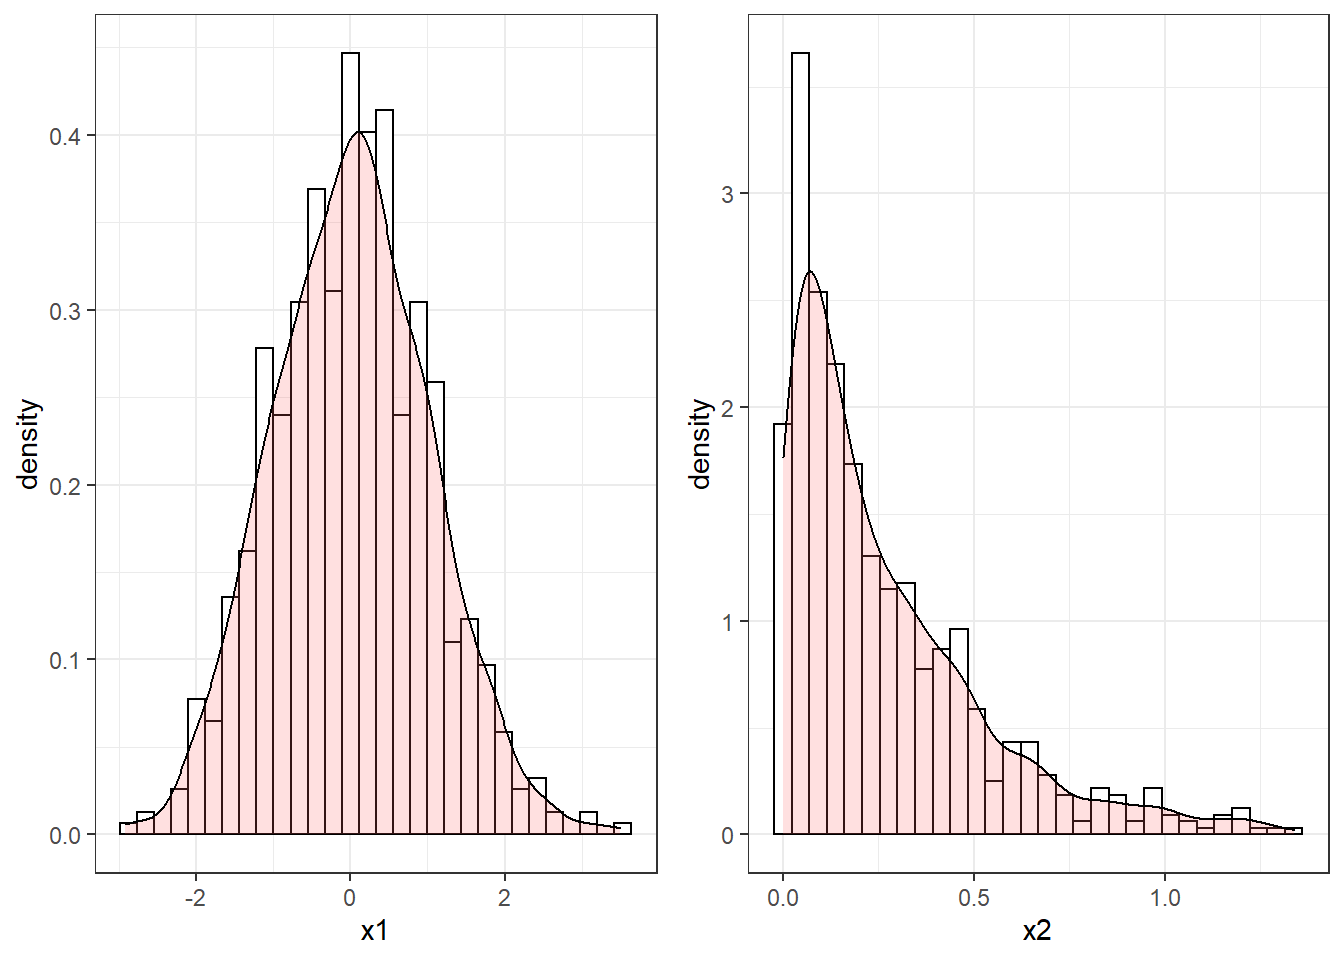
\includegraphics[width=0.5\linewidth]{SimBook_files/figure-latex/seq-1} 

}

\caption{Histograms of two sequences of randomly generated numbers}\label{fig:seq}
\end{figure}

In this chapter we will learn how to characterize randomness in a computer and how to generate numbers that appear to be random realizations of a specific random variable. We will also learn how to check if a sequence of values can be a random realization from a specific random variable.

\hypertarget{properties-of-random-numbers}{%
\section{Properties of Random Numbers}\label{properties-of-random-numbers}}

The first step to simulate numbers from a distribution is to be able to independently simulate random numbers \(u_1,u_2,\dots,u_N\) from a continuous uniform distribution between zero and one. From the previous chapter, you should remember that such a random variables has pdf
\[
f(x)=\left\{
\begin{array}{ll}
1, & 0\leq x \leq 1\\
0, &\mbox{otherwise}
\end{array}
\right.
\]
and cdf
\[
F(x)=\left\{
\begin{array}{ll}
0, & x<0\\
x, & 0\leq x \leq 1\\
1, &\mbox{otherwise}
\end{array}
\right.
\]
These two are plotted in Figure \ref{fig:uplot}.

\begin{figure}

{\centering 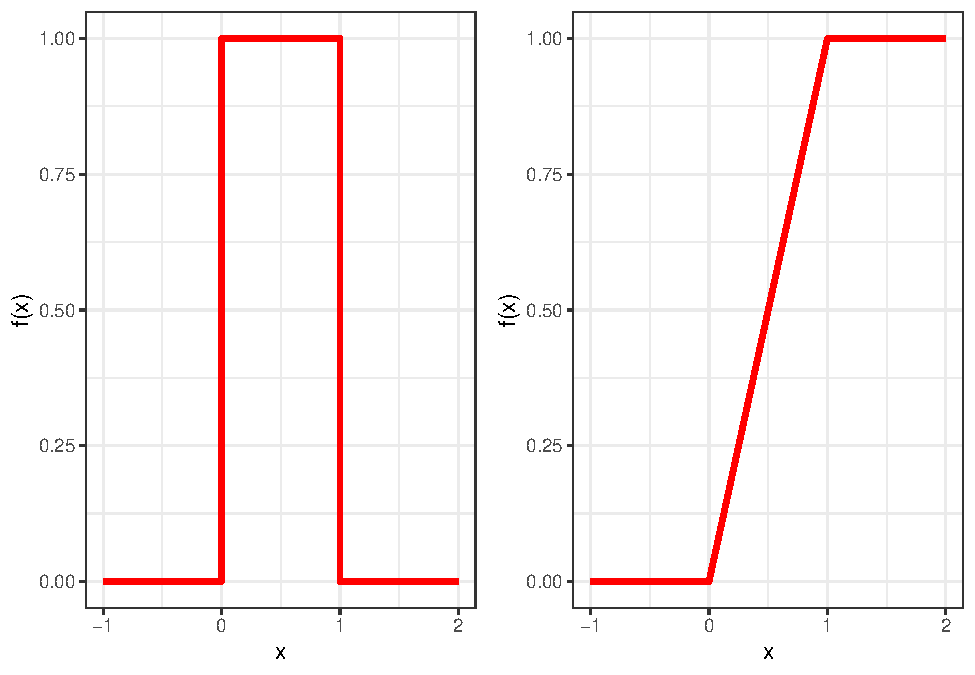
\includegraphics[width=0.5\linewidth]{SimBook_files/figure-latex/uplot-1} 

}

\caption{Pdf (left) and cdf (right) of the continuous uniform between zero and one.}\label{fig:uplot}
\end{figure}

Its expectation is 1/2 and its variance is 1/12.

This implies that if we were to divide the interval \([0,1]\) into \(n\) sub-intervals of equal length, then we would expect in each interval to have \(N/n\) observations, where \(N\) is the total number of observations.

Figure \ref{fig:uhist} shows the histograms of two sequences of numbers between zero and one: whilst the one on the left resembles the pdf of a uniform distribution, the one on the right clearly does not (it is far from being flat) and therefore it is hard to believe that such numbers follow a uniform distribution.

\begin{figure}

{\centering 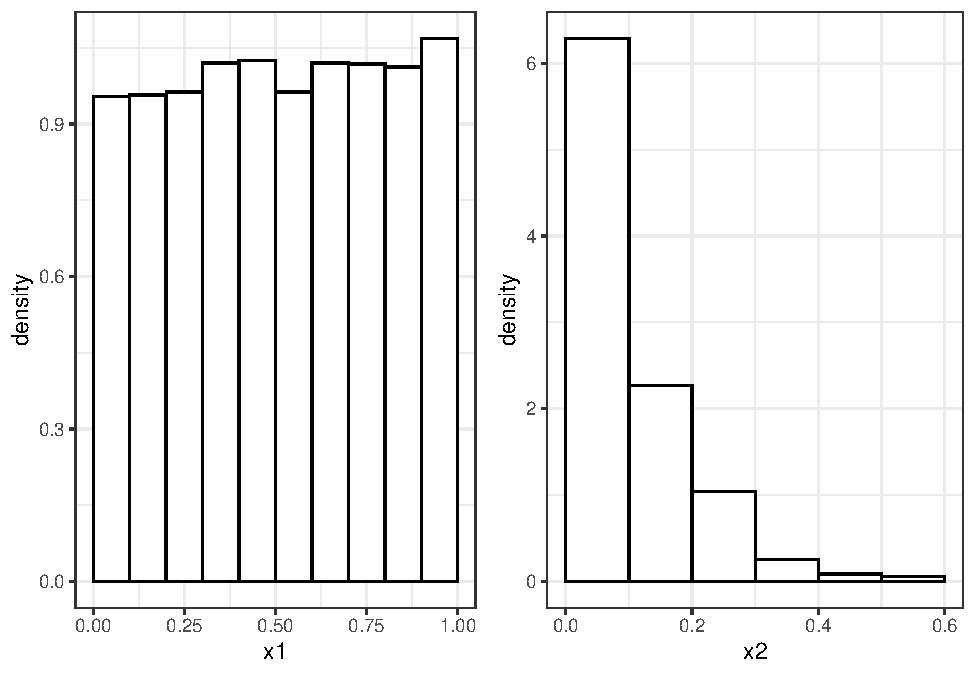
\includegraphics[width=0.5\linewidth]{SimBook_files/figure-latex/uhist-1} 

}

\caption{Histograms from two sequences of numbers between zero and one.}\label{fig:uhist}
\end{figure}

The second requirement the numbers \(u_1,\dots,u_N\) need to respect is independence. This means that the probability of observing a value in a particular sub-interval of \((0,1)\) is independent of the previous values drawn.

Consider the following sequence of numbers:
\[
\begin{array}{cccccccccc}
0.25 & 0.72 & 0.18 & 0.63 & 0.49 & 0.88 & 0.23 & 0.78 & 0.02 & 0.52
\end{array}
\]
We can notice that numbers below and above 0.5 are alternating in the sequence. We would therefore believe that after a number less than 0.5 it is much more likely to observe a number above it. This breaks the assumption of independence.

\hypertarget{pseudo-random-numbers}{%
\section{Pseudo Random Numbers}\label{pseudo-random-numbers}}

We will investigate ways to simulate numbers using algorithms in a computer. For this reason such numbers are usually called \emph{pseudo-random} numbers. Pseudo means false, in the sense that the number are not really random! They are generated according to a deterministic algorithm whose aim is to imitate as closely as possible what randomness would look like. In particular, for numbers \(u_1,\dots,u_N\) it means that they should look like independence instances of a Uniform distribution between zero and one.

Possible departures from ideal numbers are:

\begin{itemize}
\item
  the numbers are not uniformly distributed;
\item
  the mean of the numbers might not be 1/2;
\item
  the variance of the numbers might not be 1/12;
\item
  the numbers might be discrete-valued instead of continuous;
\item
  independence might not hold.
\end{itemize}

We already looked at examples of departures from the assumptions, but we will later study how to assess these departures more formally.

Before looking at how we can construct pseudo-random numbers, let's discuss some important properties/considerations that need to be taken into account when generating pseudo-random numbers:

\begin{itemize}
\item
  the random generation should be very fast. In practice, we want to use random numbers to do other computations (for example simulate a little donut shop) and such computations might be computationally intensive: if random generation were to be slow, we would not be able to perform them.
\item
  the cycle of random generated numbers should be long. The cycle is the length of the sequence before numbers start to repeat themselves.
\item
  the random numbers should be repeatable. Given a starting point of the algorithm, it should be possible to repeat the exact same sequence of numbers. This is fundamental for debugging and for reproducibility.
\item
  the method should be applicable in any programming language/platform.
\item
  and of course most importantly, the random numbers should be independent and uniformly distributed.
\end{itemize}

Repeatability of the pseudo-random numbers is worth further consideration. It is fundamental in science to be able to reproduce experiments so that the validity of results can be assessed. In R there is a specific function that allows us to do this, which is called \texttt{set.seed}. It is customary to choose as starting point of an algorithm the current year. So henceforth you will see the command:

\begin{Shaded}
\begin{Highlighting}[]
\FunctionTok{set.seed}\NormalTok{(}\DecValTok{2021}\NormalTok{)}
\end{Highlighting}
\end{Shaded}

This ensures that every time the code following \texttt{set.seed} is run, the same results will be observed. We will give below examples of this.

\hypertarget{generating-pseudo-random-numbers}{%
\section{Generating Pseudo-Random Numbers}\label{generating-pseudo-random-numbers}}

The literature on generating pseudo-random numbers is now extremely vast and it is not our purpose to review it, neither for you to learn how such algorithms work.

\hypertarget{generating-pseudo-random-numbers-in-r}{%
\subsection{Generating Pseudo-Random Numbers in R}\label{generating-pseudo-random-numbers-in-r}}

R has all the capabilities to generate such numbers. This can be done with the function \texttt{runif}, which takes one input: the number of observations to generate. So for instance:

\begin{Shaded}
\begin{Highlighting}[]
\FunctionTok{set.seed}\NormalTok{(}\DecValTok{2021}\NormalTok{)}
\FunctionTok{runif}\NormalTok{(}\DecValTok{10}\NormalTok{)}
\end{Highlighting}
\end{Shaded}

\begin{verbatim}
##  [1] 0.4512674 0.7837798 0.7096822 0.3817443 0.6363238 0.7013460 0.6404389
##  [8] 0.2666797 0.8154215 0.9829869
\end{verbatim}

generates ten random numbers between zero and one. Notice that if we repeat the same code we get the same result since we fixed the so-called \emph{seed} of the simulation.

\begin{Shaded}
\begin{Highlighting}[]
\FunctionTok{set.seed}\NormalTok{(}\DecValTok{2021}\NormalTok{)}
\FunctionTok{runif}\NormalTok{(}\DecValTok{10}\NormalTok{)}
\end{Highlighting}
\end{Shaded}

\begin{verbatim}
##  [1] 0.4512674 0.7837798 0.7096822 0.3817443 0.6363238 0.7013460 0.6404389
##  [8] 0.2666797 0.8154215 0.9829869
\end{verbatim}

Conversely, if we were to simply run the code \texttt{runif(10)} we would get a different result.

\begin{Shaded}
\begin{Highlighting}[]
\FunctionTok{runif}\NormalTok{(}\DecValTok{10}\NormalTok{)}
\end{Highlighting}
\end{Shaded}

\begin{verbatim}
##  [1] 0.02726706 0.83749040 0.60324073 0.56745337 0.82005281 0.25157128
##  [7] 0.50549403 0.86753810 0.95818157 0.54569770
\end{verbatim}

\hypertarget{linear-congruential-method}{%
\subsection{Linear Congruential Method}\label{linear-congruential-method}}

Although we will use the functions already implemented in R, it is useful to at least introduce one of the most classical algorithms to simulate random numbers, called the \emph{linear congruential method}.
This produces a sequence of integers \(x_1,x_2,x_3\) between 0 and \(m-1\) using the recursion:
\[
x_{i}=(ax_{i-1}+c)\mod m, \hspace{1cm} \mbox{for } i = 1,2,\dots
\]
Some comments:

\begin{itemize}
\item
  \(\mod m\) is the remainder of the integer division by \(m\). For instance \(5 \mod 2\) is one and \(4\mod 2\) is zero.
\item
  therefore, the algorithm generates integers between 0 and \(m-1\).
\item
  there are three parameters that need to be chosen \(a, c\) and \(m\).
\item
  the value \(x_0\) is the \emph{seed} of the algorithm.
\end{itemize}

Random numbers between zero and one can be derived by setting
\[
u_i= x_i/m.
\]

It can be shown that the method works well for specific choices of \(a\), \(c\) and \(m\), which we will not discuss here.

Let's look at an implementation.

\begin{Shaded}
\begin{Highlighting}[]
\NormalTok{lcm }\OtherTok{\textless{}{-}} \ControlFlowTok{function}\NormalTok{(N, x0, a, c, m)\{}
\NormalTok{   x }\OtherTok{\textless{}{-}} \FunctionTok{rep}\NormalTok{(}\DecValTok{0}\NormalTok{,N)}
\NormalTok{   x[}\DecValTok{1}\NormalTok{] }\OtherTok{\textless{}{-}}\NormalTok{ x0}
   \ControlFlowTok{for}\NormalTok{ (i }\ControlFlowTok{in} \DecValTok{2}\SpecialCharTok{:}\NormalTok{N) x[i] }\OtherTok{\textless{}{-}}\NormalTok{ (a}\SpecialCharTok{*}\NormalTok{x[i}\DecValTok{{-}1}\NormalTok{]}\SpecialCharTok{+}\NormalTok{c)}\SpecialCharTok{\%\%}\NormalTok{m}
\NormalTok{   u }\OtherTok{\textless{}{-}}\NormalTok{ x}\SpecialCharTok{/}\NormalTok{m}
   \FunctionTok{return}\NormalTok{(u)}
\NormalTok{\}}
\end{Highlighting}
\end{Shaded}

\begin{Shaded}
\begin{Highlighting}[]
\FunctionTok{lcm}\NormalTok{(}\AttributeTok{N =} \DecValTok{8}\NormalTok{, }\AttributeTok{x0 =} \DecValTok{4}\NormalTok{, }\AttributeTok{a =} \DecValTok{13}\NormalTok{, }\AttributeTok{c =} \DecValTok{0}\NormalTok{, }\AttributeTok{m =} \DecValTok{64}\NormalTok{)}
\end{Highlighting}
\end{Shaded}

\begin{verbatim}
## [1] 0.0625 0.8125 0.5625 0.3125 0.0625 0.8125 0.5625 0.3125
\end{verbatim}

We can see that this specific choice of parameters is quite bad: it has cycle 4! After 4 numbers the sequence repeats itself and we surely would not like to use this in practice.

In general you should not worry of these issues, R does things properly for you!

\hypertarget{testing-randomness}{%
\section{Testing Randomness}\label{testing-randomness}}

Now we turn to the following question: given a sequence of numbers \(u_1,\dots,u_N\) how can we test if they are independent realizations of a Uniform random variable between zero and one?

We therefore need to check if the distribution of the numbers is uniform and if they are actually independent.

\hypertarget{testing-uniformity}{%
\subsection{Testing Uniformity}\label{testing-uniformity}}

A simple first method to check if the numbers are uniform is to create an histogram of the data and to see if the histogram is reasonably flat. We already saw how to assess this, but let's check if \texttt{runif} works well. Simple histograms can be created in \texttt{R} using \texttt{hist} (or if you want you can use \texttt{ggplot}).

\begin{Shaded}
\begin{Highlighting}[]
\FunctionTok{set.seed}\NormalTok{(}\DecValTok{2021}\NormalTok{)}
\NormalTok{u }\OtherTok{\textless{}{-}} \FunctionTok{runif}\NormalTok{(}\DecValTok{5000}\NormalTok{)}
\FunctionTok{hist}\NormalTok{(u)}
\end{Highlighting}
\end{Shaded}

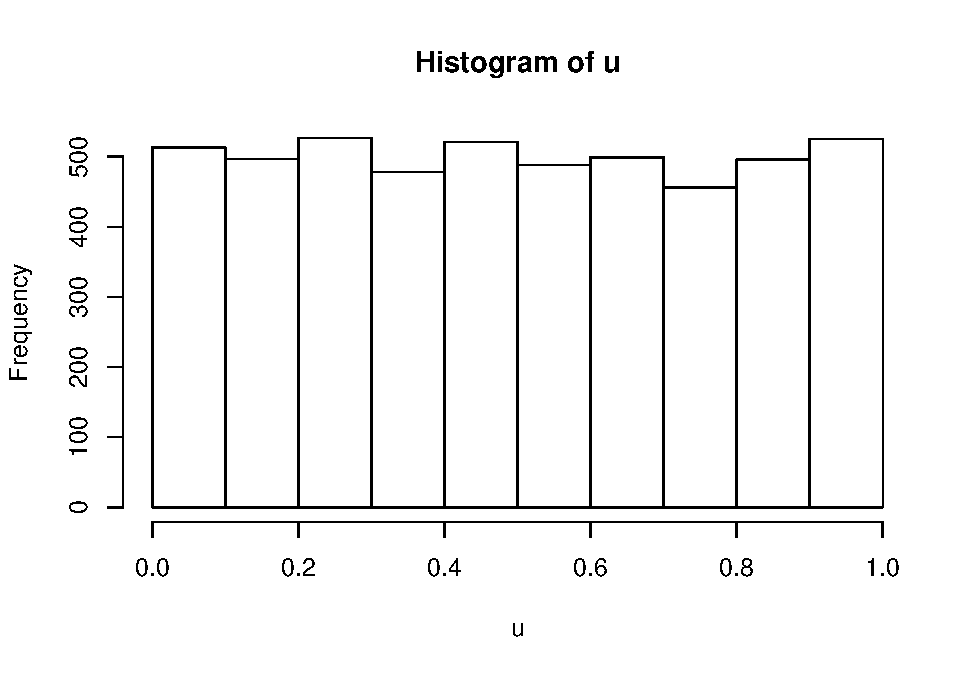
\includegraphics{SimBook_files/figure-latex/unnamed-chunk-81-1.pdf}

We can see that the histogram is reasonably flat and therefore the assumption of uniformity seems to hold.

Although the histogram is quite informative, it is not a fairly formal method. We could on the other hand look at tests of hypotheses of this form:
\begin{align*}
H_0: & \;\;u_i \mbox{ is uniform between zero and one, } i=1,2,\dots\\
H_a: & \;\;u_i \mbox{ is not uniform between zero and one, } i=1,2,\dots\\
\end{align*}

The null hypothesis is thus that the numbers are indeed uniform, whilst the alternative states that the numbers are not. If we reject the null hypothesis, which happens if the p-value of the test is very small (or smaller than a critical value \(\alpha\) of our choice), then we would believe that the sequence of numbers is not uniform.

There are various ways to carry out such a test, but we will consider here only one: the so-called \emph{Kolmogorov-Smirnov Test}. We will not give all details of this test, but only its interpretation and implementation.

In order to understand how the test works we need to briefly introduce the concept of \emph{empirical cumulative distribution function} or \emph{ecdf}. The ecdf \(\hat{F}\) is the cumulative distribution function computed from a sequence of \(N\) numbers as
\[
\hat{F}(t)= \frac{\mbox{numbers in the sequence }\leq t}{N}
\]

Let's consider the following example.

\begin{Shaded}
\begin{Highlighting}[]
\NormalTok{data }\OtherTok{\textless{}{-}} \FunctionTok{data.frame}\NormalTok{(}\AttributeTok{u=} \FunctionTok{c}\NormalTok{(}\FloatTok{0.1}\NormalTok{,}\FloatTok{0.2}\NormalTok{,}\FloatTok{0.4}\NormalTok{,}\FloatTok{0.8}\NormalTok{,}\FloatTok{0.9}\NormalTok{))}
\FunctionTok{ggplot}\NormalTok{(data,}\FunctionTok{aes}\NormalTok{(u)) }\SpecialCharTok{+} \FunctionTok{stat\_ecdf}\NormalTok{(}\AttributeTok{geom =} \StringTok{"step"}\NormalTok{) }\SpecialCharTok{+} \FunctionTok{theme\_bw}\NormalTok{() }\SpecialCharTok{+} \FunctionTok{ylab}\NormalTok{(}\StringTok{"ECDF"}\NormalTok{)}
\end{Highlighting}
\end{Shaded}

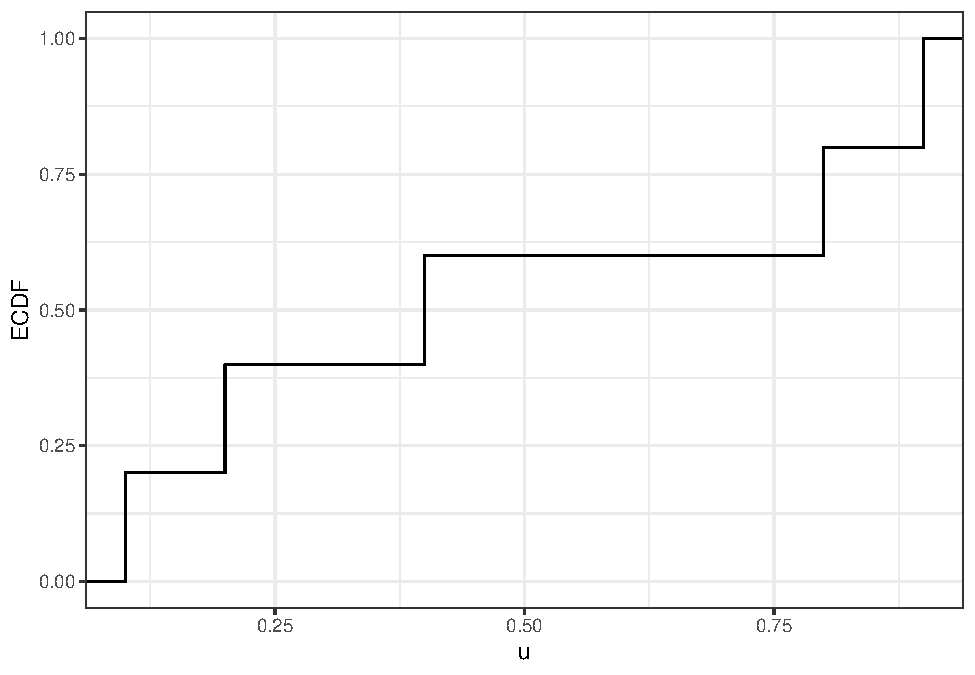
\includegraphics{SimBook_files/figure-latex/unnamed-chunk-82-1.pdf}

For instance, since there are 3 numbers out of 5 in the vector \texttt{u} that are less than 0.7, then \(\hat{F}(0.7)=3/5\).

The idea behind the Kolmogorov-Smirnov test is to quantify how similar the ecdf computed from a sequence of data is to the one of the uniform distribution which is represented by a straight line (see Figure \ref{fig:uplot}).

As an example consider Figure \ref{fig:Kol}.

\begin{Shaded}
\begin{Highlighting}[]
\NormalTok{u1 }\OtherTok{\textless{}{-}} \FunctionTok{runif}\NormalTok{(}\DecValTok{20}\NormalTok{)}
\NormalTok{u2 }\OtherTok{\textless{}{-}} \FunctionTok{rexp}\NormalTok{(}\DecValTok{20}\NormalTok{,}\DecValTok{10}\NormalTok{)}
\NormalTok{u2 }\OtherTok{\textless{}{-}}\NormalTok{ u2[u2}\SpecialCharTok{\textless{}=}\DecValTok{1}\NormalTok{]}
\FunctionTok{ggplot}\NormalTok{(}\FunctionTok{data.frame}\NormalTok{(}\AttributeTok{u1=}\NormalTok{u1),}\FunctionTok{aes}\NormalTok{(u1)) }\SpecialCharTok{+} \FunctionTok{stat\_ecdf}\NormalTok{(}\AttributeTok{geom =} \StringTok{"step"}\NormalTok{) }\SpecialCharTok{+} \FunctionTok{theme\_bw}\NormalTok{() }\SpecialCharTok{+} \FunctionTok{ylab}\NormalTok{(}\StringTok{"ECDF"}\NormalTok{) }\SpecialCharTok{+} \FunctionTok{geom\_abline}\NormalTok{(}\AttributeTok{intercept =} \DecValTok{0}\NormalTok{, }\AttributeTok{slope =} \DecValTok{1}\NormalTok{)}
\end{Highlighting}
\end{Shaded}

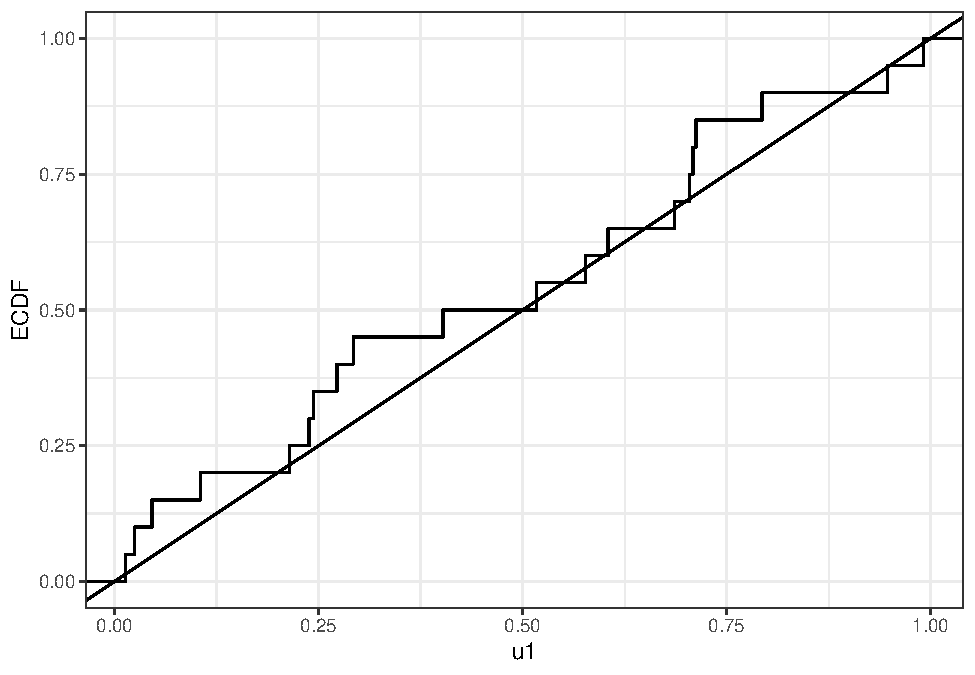
\includegraphics{SimBook_files/figure-latex/unnamed-chunk-83-1.pdf}

\hypertarget{testing-independence}{%
\subsection{Testing Independence}\label{testing-independence}}

\hypertarget{random-variate-generation}{%
\section{Random Variate Generation}\label{random-variate-generation}}

  \bibliography{book.bib,packages.bib}

\end{document}
